%\documentclass[12pt]{scrreprt}
\documentclass[12pt]{report} 

% language may be romanian or english (default is english)
% type may be bachelor or master (default is bachelor)
\usepackage[language=english, type=bachelor]{style}

%\geometry{a4paper,top=2.5cm,left=3cm,right=2.5cm,bottom=2.5cm}
%in style
%controlling the appearance of your headers and footers
\usepackage{fancyhdr}
\usepackage{pgfplots}
\usepackage{amsmath} 
\usetikzlibrary{positioning, arrows.meta, shapes.geometric}
\pagestyle{fancy}
\lhead{}
\chead{}
\renewcommand{\headrulewidth}{0.2pt}
\renewcommand{\footrulewidth}{0.2pt}
\setcounter{secnumdepth}{3}
\setcounter{tocdepth}{3}

\begin{document}

\makeatletter
\setbool{@eng}{false}
\makeatother

\specialization{INFORMATICĂ}
\title{Reducerea costurilor de cloud în streamingul muzical prin livrare peer-to-peer}
\author{Darius-George Sala}
\supervisor{Dr. Lect. Prof. Mircea Ioan-Gabriel}
\maketitle

\makeatletter
\setbool{@eng}{true}
\makeatother

\specialization{COMPUTER SCIENCE}
\title{Reducing Cloud Costs in Music Streaming with Peer-Assisted Delivery}
\author{Darius-George Sala}
\supervisor{Dr. Lect. Prof. Mircea Ioan-Gabriel}
\maketitle

\newpage
\pagenumbering{roman}

\cleardoublepage
ABSTRACT
\vspace{0.5cm}
\hrule
\vspace{0.5cm}
%\cleardoublepage
{\bfseries
This thesis studies how the cloud egress cost of on-demand music streaming can be reduced without changing the listener's experience. The egress bill grows with the size of the audience rather than the revenue it brings, yet a listener who has just received a piece of a song already holds a valid copy that another listener starting the same song shortly after may need, so the audience itself already contains a possible delivery network. The proposed solution is a peer-assisted streaming system in which the server delivers a small initial prefix of each song and stays available as a fallback, while the rest of the audio is delivered directly between listeners through WebRTC, moving the origin away from serving $O(N)$ full copies and toward a small bootstrap-and-fallback role.

\par The original contribution is the design, implementation and evaluation of a single cross-platform prototype, MP33r, that combines a dynamic 5\% server prefix, 64 KiB content-addressed (SHA-256) chunks verified on the client regardless of source, round-trip-time and throughput-based peer ranking, an always-present server fallback and multi-replica signaling into one working system, with a Spring Boot backend and a Flutter client running on Linux, macOS, Windows, Android, iOS and the web. In the measured warm-swarm scenario, two to five listeners received 88.4\% of their bytes from peers while the origin share stayed flat as listeners grew, and the prefix hid the median 243 ms WebRTC setup time, keeping click-to-sound latency at the level of a normal server stream. These controlled single-machine results validate the mechanism and the cost model rather than serving as production measurements, supporting the conclusion that listeners can act as part of a song's delivery infrastructure as long as the system preserves instant playback, verifies untrusted chunks and keeps a reliable server fallback.
}



\tableofcontents


\cleardoublepage
\markboth{}{}
INTRODUCTION
\vspace{0.5cm}
\hrule
\vspace{0.5cm}

Every time a song is played from a cloud-hosted streaming service, the provider pays for the same bytes in two different ways: first to store and process them, and then again when they leave the data centre. That second cost, usually called egress, grows with the number of listeners, not with how much money those listeners bring in. This means that a song becoming popular is good news and bad news at the same time: more people are listening, but the delivery bill is also rising. Large providers can absorb this through scale, contracts and CDNs, but the basic shape of the problem remains very simple. Double the audience, and the origin has to serve roughly double the data.

\par The interesting part is that the problem already contains a possible delivery network. A listener who has just received a piece of a song has a valid copy of that piece, and another listener starting the same song shortly after may need exactly those bytes. If clients can safely pass chunks between themselves, the origin server no longer has to be the source of every byte. It can become the component that starts playback, seeds the swarm and stays available when peers are missing. The hard part is making this happen without turning the user experience into an experiment. Playback still has to start quickly, the same client has to work on desktop, mobile and the web, and a chunk received from another user has to be checked as strictly as a chunk received from the server. This thesis designs, builds and measures a music streaming system around those constraints, moving the origin away from serving $O(N)$ full copies of the same song and toward a small bootstrap-and-fallback role in the ideal case.

\par The thesis is organised into five chapters. Chapter \ref{intro} sets out the problem context and surveys the related work, breaking peer-assisted streaming into five design domains: latency, connectivity, storage, integrity and flow control. It weighs the candidate solutions for each of them and reviews the prior systems that inform the design, without yet committing to one. Chapter \ref{chap:ch2} turns those trade-offs into a formal cost model, derives the system's key parameters, including the 64 KiB chunk and the dynamic 5\% prefix, and commits to the synthesised architecture that the rest of the thesis implements and evaluates. Chapter \ref{chap:ch3} presents the implementation in three parts: the architecture and its layers, the runtime flows together with the testing approach, and the user interface. Chapter \ref{chap:ch4} evaluates the working prototype by measuring egress offload, startup latency and scaling as the audience grows, then places the results next to the systems from the literature. Chapter \ref{chap:ch5} closes the loop with the conclusions and the directions for future work.

\vspace{1cm}
\par The original contributions of this work are the following:
\begin{itemize}
  \item \textbf{a dynamic prefix-caching bootstrap}, serving roughly 5\% of each song from the origin, that hides the WebRTC connection setup so playback can start while the peer mesh forms in the background;
  \item \textbf{a WebRTC data-channel peer transport} with round-trip time and throughput-based peer ranking, staggered fan-out and an always-present server fallback, deliberately built without a TURN relay so the cost-saving property of the peer model is preserved, combined with a 64 KiB content-addressed (SHA-256) chunking scheme that deduplicates storage on the server and lets the client verify every chunk in the same way, whether it arrived from a peer or from the origin;
  \item \textbf{an end-to-end evaluation}, built on a purpose-made headless measurement client, that quantifies the egress saving, validates the cost model, and uncovered a signaling concurrency bottleneck that was capping multi-peer scaling.
\end{itemize}


\vspace{1cm}
\markboth{}{}
DECLARATION OF GENERATIVE AI AND AI-ASSISTED TECHNLOGIES IN THE WRITING PROCESS
\vspace{0.5cm}
\hrule
\vspace{0.5cm}
\par During the preparation of this work, the author used Gemini to check grammar, refine and improve the academic tone of the text. After using this tool, the author reviewed and edited the content as needed and takes full responsibility for the final thesis.


\newpage
\pagenumbering{arabic}

\chapter{Problem Context and Related Work}

%\chapter*{Introducere}
\label{intro}

\tolerance=9999
\emergencystretch=3em

\indent \par This chapter sets the stage for the rest of the thesis. It starts with the problem itself: why delivering on-demand audio from the cloud has become expensive, and why the egress bandwidth bill is the part worth attacking first. It then breaks peer-assisted streaming into the handful of design domains that any such system has to handle, surveys the candidate solutions for each one, and reviews the older systems that combined them. The aim here is deliberately limited to mapping the design space and weighing the trade-offs, as the quantitative argument that turns those trade-offs into one committed design is the work of Chapter \ref{chap:ch2}.

\section{Problem Context}

\indent \par On-demand multimedia streaming has changed the way people consume music and video, but it has also made delivery costs harder to ignore. Most streaming platforms still depend on centralised cloud infrastructure and CDNs (Content Delivery Networks). Every request to listen to a song creates a small bandwidth fee for the provider, usually called egress, and that small fee grows into a serious bill when the user base grows. This cost model is not hidden in fine print: AWS, Google Cloud and Azure all expose public data-transfer-out pricing pages, treating bytes leaving the cloud as a first-class billable resource \cite{aws_global_network_faq,google_cloud_network_pricing,azure_bandwidth_pricing}.

\par For a while, this problem was manageable. The rapid growth of AI workloads has changed the industry quickly, and cloud capacity has become a harder financial problem for companies that already move a lot of data. Modern streaming services use machine learning for real-time recommendation, user sentiment analysis, adaptive bitrate optimisation and predictive analytics. These systems improve the user experience, but they also compete for the same cloud resources and push operating costs upward.

\par Back in 2018, Spotify signed a deal with Google to spend a minimum of \$447 million on the Google Cloud Platform during the first three years of service \cite{spotify_google}. Over the same period shown in Figure \ref{fig:spotify_economics_indexed}, Spotify Premium moved from \$9.99 in 2018 to \$12.99 in 2025 \cite{spotify_prices}, after several consecutive increases. The reasons are not limited to bandwidth, of course, but rising operating costs, pandemic-era inflation and AI workloads competing for the same cloud capacity all squeeze provider margins and are eventually felt by the end consumer. The egress bandwidth targeted in this thesis has a cleaner shape: it is billed per gigabyte and scales with the number of listeners, regardless of those wider price movements. That is what makes it worth attacking directly. If streaming is to stay economically reasonable, the delivery path has to become cheaper for the provider without becoming worse for the listener.

\par The irony is that peer-assisted delivery is not foreign to music streaming. Before its full cloud migration, Spotify itself used a low-latency P2P music-on-demand architecture, measured by Kreitz and Niemel\"a as a large-scale production system \cite{spotify_p2p}. Later work on integrating smartphones into the same peer-assisted model showed why mobile devices cannot simply be treated as desktop peers, especially when battery state and radio access change during the day \cite{spotify_mobile_p2p}. The goal here is therefore not to reinvent generic file sharing, but to recover the useful part of that older architecture under modern browser, mobile and cloud constraints.

\begin{figure}[htbp]
    \centering
    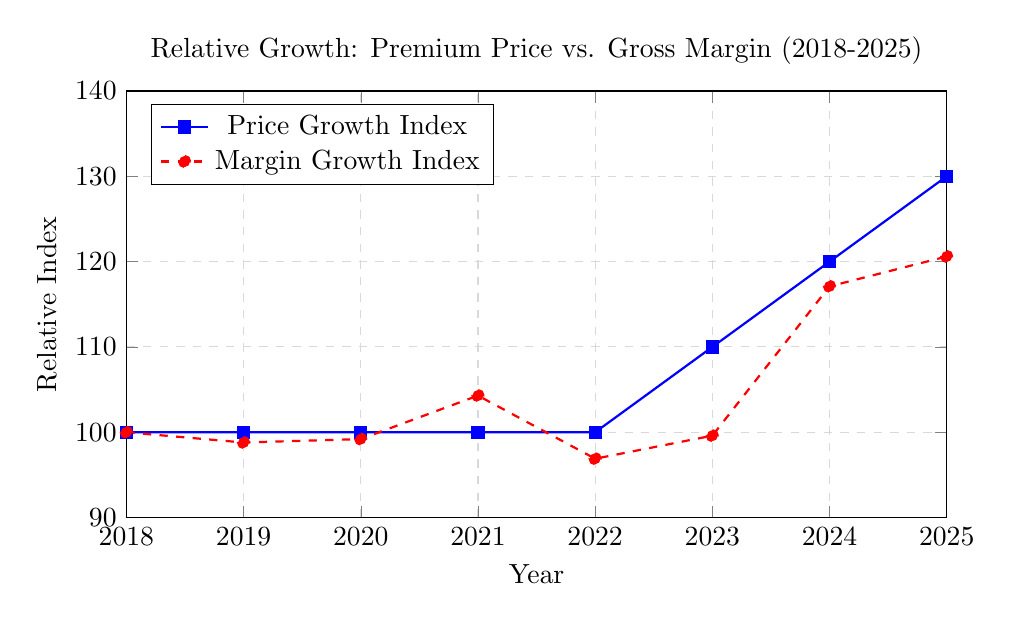
\begin{tikzpicture}
        \begin{axis}[
            width=12cm, height=7cm,
            xmin=2018, xmax=2025,
            ymin=90, ymax=140,
            xtick={2018, 2019, 2020, 2021, 2022, 2023, 2024, 2025},
            x tick label style={/pgf/number format/1000 sep=},
            ytick={90, 100, 110, 120, 130, 140},
            ylabel={Relative Index},
            xlabel={Year},
            title={Relative Growth: Premium Price vs. Gross Margin (2018-2025)},
            legend pos=north west,
            grid=both,
            grid style={dashed, gray!30}
        ]

        % Price Indexed: (Current Price / 9.99) * 100
        \addplot[
            color=blue,
            mark=square*,
            thick
        ] coordinates {
            (2018, 100.0)
            (2019, 100.0)
            (2020, 100.0)
            (2021, 100.0)
            (2022, 100.0)
            (2023, 110.0) % 10.99 / 9.99
            (2024, 120.0) % 11.99 / 9.99
            (2025, 130.0) % 12.99 / 9.99
        };
        \addlegendentry{Price Growth Index}

        % Margin Indexed: (Current Margin / 25.7) * 100
        \addplot[
            color=red,
            mark=*,
            thick,
            dashed
        ] coordinates {
            (2018, 100.0)
            (2019, 98.8)  % 25.4 / 25.7
            (2020, 99.2)  % 25.5 / 25.7
            (2021, 104.3) % 26.8 / 25.7
            (2022, 96.9)  % 24.9 / 25.7
            (2023, 99.6)  % 25.6 / 25.7
            (2024, 117.1) % 30.1 / 25.7
            (2025, 120.6) % 31.0 / 25.7
        };
        \addlegendentry{Margin Growth Index}

        \end{axis}
    \end{tikzpicture}
    \caption{Relative growth index of Spotify's Premium Price \cite{spotify_prices} and Gross Profit Margin \cite{spotify_gross_margin}, normalised to a base value of 100 in the year 2018.}
    \label{fig:spotify_economics_indexed}
\end{figure}

\par In an effort to ease the load on cloud infrastructure, the academic community has explored decoupled network models, including hybrid CDN-P2P systems and peer-assisted CDNs \cite{hybrid_cdn_p2p,pa_cdn_survey}. Translating these architectures into a working system, however, means meeting the same recurring design problems. The system has to hide latency so playback starts when the listener presses play, even though peers still have to be found and connected. It has to establish direct peer-to-peer links across NATs, firewalls and the browser security sandbox, on native and web platforms alike. It has to decide what the client stores and for how long, balancing network offload against device storage and battery. It has to segment and verify audio so that bytes from an untrusted peer are as safe as bytes from the server. Finally, it has to react to fluctuating peer performance without stalling playback or fragmenting the shared data across the swarm.

\par Each of the following sections takes one of these domains in turn and weighs the leading candidate solutions against each other. The order roughly follows the path of a single chunk through the system, from the moment playback is requested to the moment the bytes are verified and played. None of the domains is treated in isolation, because a decision taken in one of them quietly constrains the choices left in the others. A final section then steps back to look at how complete systems have combined these choices in practice.

\section{Achieving Near-Instant Playback}
\indent \par The first requirement of a modern streaming service is simple to state and hard to satisfy: playback has to start quickly. A listener who presses play does not think about peer discovery, buffer maps or NAT traversal. They expect sound, and they expect it now. A system that is correct in every other respect but slow to start will still feel broken, so this requirement has to be satisfied before any of the others can matter.

\par A download-first approach is therefore a bad fit for streaming. If a listener has to wait for the whole file, even a technically correct system feels broken. Research on Quality of Experience (QoE) supports the same intuition: in the large-scale study by Krishnan and Sitaraman, users begin abandoning streaming content rapidly when startup delays exceed only a few seconds, with the penalty becoming visible around the two-second mark \cite{quality_impact}. The lesson is that startup latency is not a secondary metric to be tuned later, but a hard constraint that shapes the delivery architecture from the outset.

\begin{figure}[htbp]
    \centering
    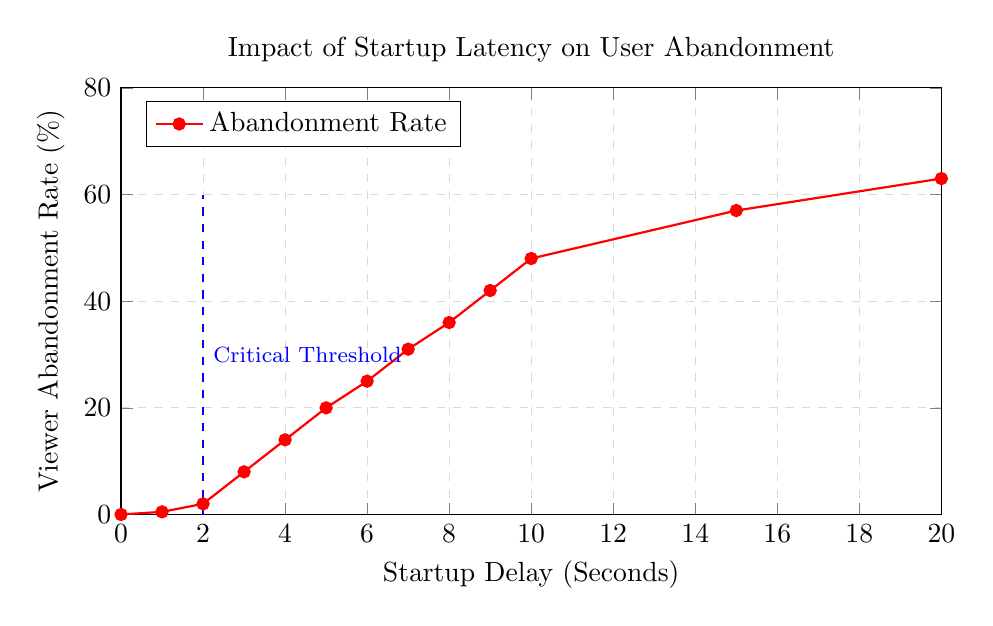
\begin{tikzpicture}
        \begin{axis}[
            width=12cm, height=7cm,
            xlabel={Startup Delay (Seconds)},
            ylabel={Viewer Abandonment Rate (\%)},
            xmin=0, xmax=20,
            ymin=0, ymax=80,
            grid=both,
            grid style={dashed, gray!30},
            title={Impact of Startup Latency on User Abandonment},
            legend pos=north west
        ]

        \addplot[
            color=red,
            mark=*,
            thick
        ] coordinates {
            (0, 0)
            (1, 0.5)
            (2, 2)
            (3, 8)
            (4, 14)
            (5, 20)
            (6, 25)
            (7, 31)
            (8, 36)
            (9, 42)
            (10, 48)
            (15, 57)
            (20, 63)
        };
        \addlegendentry{Abandonment Rate}

        \draw[dashed, thick, blue] (axis cs:2,0) -- (axis cs:2,60) node[midway, right, font=\footnotesize] {Critical Threshold};

        \end{axis}
    \end{tikzpicture}
    \caption{Viewer abandonment rate as a function of startup delay\cite{quality_impact}.}
    \label{fig:latency_abandonment}
\end{figure}

\par The architecture therefore has to use progressive delivery. The listener should perceive near-instant playback, while the system quietly prepares the slower parts of the delivery path in the background. Both of the techniques below try to remove the wait the listener would otherwise see, but they place that preparatory work at different points in time and pay for it in different ways. The two main strategies considered here are prefix caching and predictive pre-fetching.

\subsection{Prefix Caching}
\indent \par Prefix caching means that the server immediately sends the first part of the content while the P2P connection is established in the background for the rest. The idea is well known in multimedia proxy work: by storing the first seconds of a clip, the proxy can hide the delay and throughput variation of the slower path \cite{prefix_caching}. The first part of the file is the only segment whose timing the listener perceives directly, so guaranteeing it from a fast, reliable source is enough to make playback feel instant. Everything after it can be assembled more slowly, as long as it arrives before the prefix runs out.

\par This method gives the user a reliable start from the server and masks the P2P connection setup time. It also absorbs the initial demand burst and acts as a fail-safe, because the server can continue streaming the whole track if peers are unavailable. The downside is that prefix caching adds server storage and byte-range complexity, and it creates one sensitive boundary: the transition from the server prefix to the peer-supplied chunks. If that transition is not synchronised, the listener may hear clicks, silence or other artefacts.

\subsection{Predictive Pre-Fetching}
\indent \par Predictive pre-fetching is, at least on paper, a good alternative to prefix caching. It uses a prediction model to guess the user's next choice, then downloads that content in the background before the user reaches it. The wait disappears entirely when the guess is correct, because the content is already on the device by the time it is requested. The whole approach therefore rises or falls on the quality of the prediction, which is where its weaknesses appear.

\par This method can remove the buffering issue, keep startup delay close to zero, and even allow offline playback if the connection drops after the content was fetched. It also brings obvious waste. The client may fill storage with media the user never plays, the system may consume bandwidth for wrong predictions, and the cloud may still pay for bytes that helped nobody. As evaluated by Krishnamoorthi et al., pre-fetching can reduce startup time for likely next videos, but only when the client carefully balances aggressiveness against bandwidth use and the quality of the video that is already playing \cite{bandwidth_aware_prefetching}.


\begin{figure}[htbp]
    \centering
    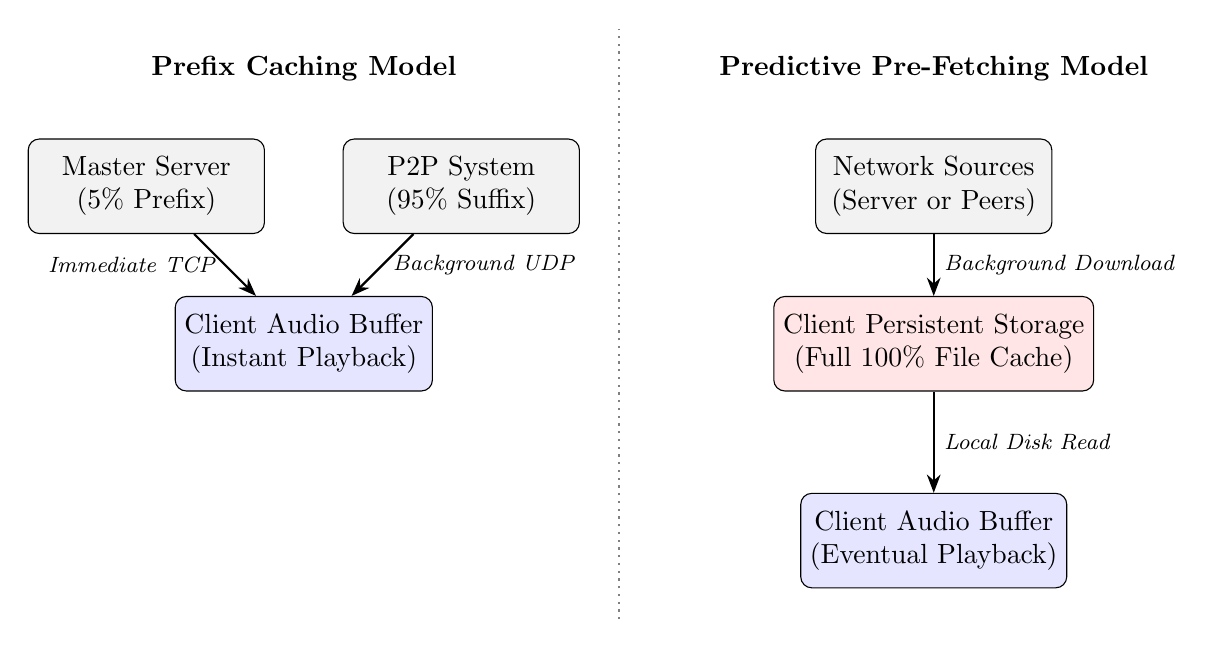
\begin{tikzpicture}[
        node distance=2cm,
        box/.style={draw, rectangle, minimum width=3cm, minimum height=1.2cm, align=center, fill=gray!10, rounded corners},
        arrow/.style={->, >=Stealth, thick},
        label_text/.style={font=\footnotesize\itshape}
    ]
        \node[font=\bfseries] (title_prefix) at (0, 3.5) {Prefix Caching Model};
        \node[box] (server_prefix) at (-2, 2) {Master Server\\(5\% Prefix)};
        \node[box] (peer_prefix) at (2, 2) {P2P System\\(95\% Suffix)};
        \node[box, fill=blue!10] (buffer_prefix) at (0, 0) {Client Audio Buffer\\(Instant Playback)};

        \draw[arrow] (server_prefix) -- node[left, label_text] {Immediate TCP} (buffer_prefix);
        \draw[arrow] (peer_prefix) -- node[right, label_text] {Background UDP} (buffer_prefix);

        \node[font=\bfseries] (title_predict) at (8, 3.5) {Predictive Pre-Fetching Model};
        \node[box] (network_predict) at (8, 2) {Network Sources\\(Server or Peers)};
        \node[box, fill=red!10] (storage_predict) at (8, 0) {Client Persistent Storage\\(Full 100\% File Cache)};
        \node[box, fill=blue!10] (buffer_predict) at (8, -2.5) {Client Audio Buffer\\(Eventual Playback)};

        \draw[arrow] (network_predict) -- node[right, label_text] {Background Download} (storage_predict);
        \draw[arrow] (storage_predict) -- node[right, label_text] {Local Disk Read} (buffer_predict);
        \draw[thick, dotted, gray] (4, -3.5) -- (4, 4);

    \end{tikzpicture}
    \caption{Data-flow comparison of Prefix Caching vs Predictive Pre-Fetching.}
    \label{fig:caching_comparison}
\end{figure}

\section{Bridging Native And Browser Environments}
\indent \par Peer-assisted streaming only works if peers can actually reach each other. That sounds obvious, but it becomes difficult when the same application has to run both as a native program and inside a web browser. Native operating systems expose socket APIs that allow direct access to TCP and UDP \cite{top_down_cn}. Browsers, for good security reasons, do not.

\par A system that uses one networking protocol on native clients and another in the browser is fragile from the start. The browser sandbox forbids arbitrary sockets to untrusted peers, because otherwise a web page would become a very convenient attack tool \cite{webrtc_security}. Rescorla's WebRTC security architecture makes the same point plainly: without protocol-level cryptographic safeguards, unauthenticated peers cannot be trusted \cite{webrtc_security}. In this context, an architecture that cannot merge native and browser clients cannot deliver cross-platform P2P streaming at all.

\par The transport therefore has to navigate complex network topologies without violating the security model of any platform. The system needs one peer swarm, not a desktop swarm, a mobile swarm and a browser island. A fragmented swarm would split the pool of peers holding any given chunk, which directly weakens the offload the whole design depends on. The main candidate for this role is Web Real-Time Communication (WebRTC), with relay-only delivery through TURN or proxy servers kept as the contrasting option.

\subsection{Web Real-Time Communication (WebRTC)}
\indent \par WebRTC offers mandatory security through Datagram Transport Layer Security (DTLS) and includes built-in Network Address Translation (NAT) traversal mechanisms such as Interactive Connectivity Establishment (ICE, not to be confused with whatever the USA is doing nowadays) and Session Traversal Utilities for NAT (STUN). The W3C WebRTC Recommendation standardises the browser API for exchanging media and generic application data between browsers or compatible devices, while ICE itself is defined as the NAT traversal procedure that searches for a usable path between peers \cite{webrtc_w3c,ice_rfc8445}. The decisive property for this thesis is that the same standard is implemented by every major browser and by the native libraries the client uses, so a single connection model works across all the target platforms. Connectivity and security therefore come from the protocol itself rather than from anything the application has to build by hand.

\par This lets devices on private networks communicate over the public internet without browser plugins. For this thesis, the important part is the DataChannel: the IETF specification places generic peer data on SCTP over DTLS, which is exactly the reliable ordered transport needed for chunk requests and responses \cite{webrtc_data_channels}. WebRTC is not perfect, though. It adds connection setup overhead, consumes CPU on the client, and requires a signaling server to coordinate the offer, answer and ICE candidate exchange (see Figure \ref{fig:webrtc_architecture}). Researchers at Universidad Rey Juan Carlos measured mean latencies of around 200 ms without packet loss and around 400 ms in a second experiment, while also noting that the UDP-based approach loses scalability when many clients are introduced \cite{webrtc_testing}.

\begin{figure}[htbp]
    \centering
    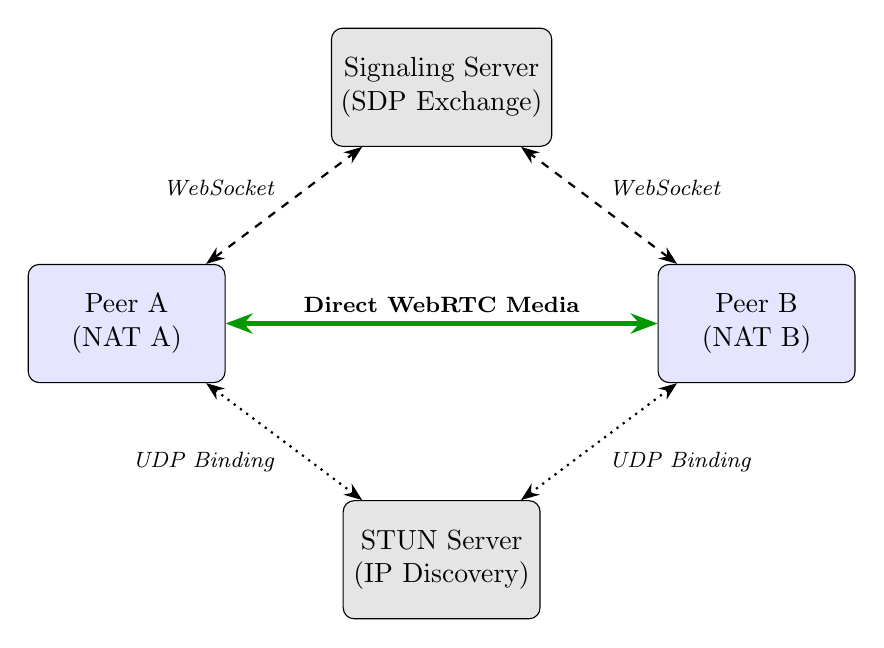
\begin{tikzpicture}[
        node distance=2.5cm,
        client/.style={draw, rectangle, minimum width=2.5cm, minimum height=1.5cm, align=center, fill=blue!10, rounded corners},
        server/.style={draw, rectangle, minimum width=2.5cm, minimum height=1.5cm, align=center, fill=gray!20, rounded corners},
        arrow/.style={->, >=Stealth, thick},
        biarrow/.style={<->, >=Stealth, thick},
        label_text/.style={font=\footnotesize\itshape}
    ]

        \node[client] (peerA) at (0, 0) {Peer A\\(NAT A)};
        \node[client] (peerB) at (8, 0) {Peer B\\(NAT B)};

        \node[server] (signaling) at (4, 3) {Signaling Server\\(SDP Exchange)};
        \node[server] (stun) at (4, -3) {STUN Server\\(IP Discovery)};

        \draw[biarrow, dashed] (peerA) -- node[above left, label_text] {WebSocket} (signaling);
        \draw[biarrow, dashed] (peerB) -- node[above right, label_text] {WebSocket} (signaling);

        \draw[biarrow, dotted] (peerA) -- node[below left, label_text] {UDP Binding} (stun);
        \draw[biarrow, dotted] (peerB) -- node[below right, label_text] {UDP Binding} (stun);

        \draw[biarrow, draw=green!60!black, line width=1.5pt] (peerA) -- node[above, font=\bfseries\footnotesize] {Direct WebRTC Media} (peerB);

    \end{tikzpicture}
    \caption{WebRTC architecture.}
    \label{fig:webrtc_architecture}
\end{figure}

\subsection{'Relay-Only' (TURN/Proxy Servers)}
\indent \par Relay-only delivery takes the opposite route. It guarantees connectivity by routing all P2P traffic through Traversal Using Relays around NAT (TURN) or proxy servers (see Figure \ref{fig:turn_architecture}). TURN provides a reliable relay for peers behind restrictive symmetric NATs or enterprise firewalls that block direct UDP communication \cite{relays_turn}. Because the relay sits in the data path for every transfer, connectivity stops being a question the application has to solve case by case, which is the entire appeal of the approach.

\par This simplifies the client and makes connection monitoring easier, but it also moves the bandwidth bill back to infrastructure controlled by the provider. Every relayed byte is paid for like a server byte, which weakens the main reason for using P2P in the first place. It also adds a central point of failure to the P2P component, which is especially undesirable for content streaming. For a system whose whole purpose is to push bytes off the provider's infrastructure, a transport that routes those same bytes back through it is self-defeating, which is why this thesis keeps TURN only as a conceptual contrast and never relies on it.

\begin{figure}[htbp]
    \centering
    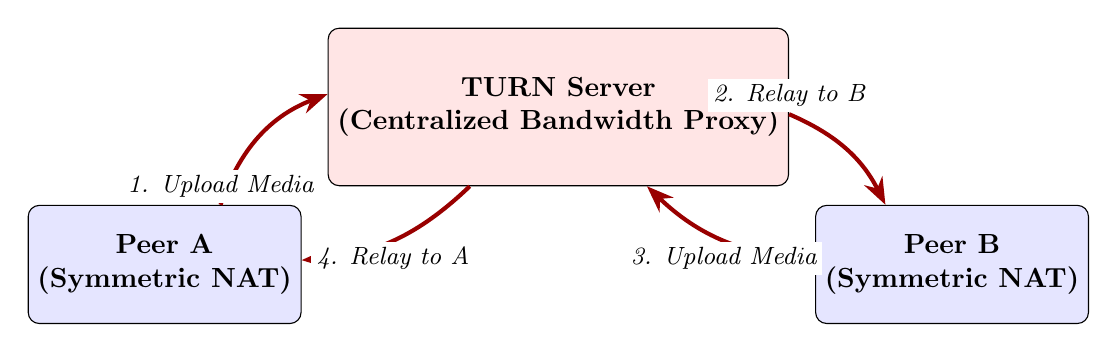
\begin{tikzpicture}[
        node distance=3cm,
        client/.style={draw, rectangle, minimum width=3cm, minimum height=1.5cm, align=center, fill=blue!10, rounded corners, font=\bfseries},
        server/.style={draw, rectangle, minimum width=3.5cm, minimum height=2cm, align=center, fill=red!10, rounded corners, font=\bfseries},
        arrow/.style={->, >=Stealth, thick, draw=red!60!black, line width=1.5pt},
        label_text/.style={font=\small\itshape, align=center, fill=white, inner sep=2pt}
    ]
        \node[client] (peerA) at (0, 0) {Peer A\\(Symmetric NAT)};
        \node[client] (peerB) at (10, 0) {Peer B\\(Symmetric NAT)};
        \node[server] (turn) at (5, 2) {TURN Server\\(Centralized Bandwidth Proxy)};

        \draw[arrow] (peerA) to[bend left=25] node[above, label_text, pos=0.0] {1. Upload Media} (turn);
        \draw[arrow] (turn) to[bend left=20] node[above, label_text, pos=0.0] {2. Relay to B} (peerB);
        \draw[arrow] (peerB) to[bend left=20] node[below, label_text, pos=0.5] {3. Upload Media} (turn);
        \draw[arrow] (turn) to[bend left=20] node[below, label_text, pos=0.5] {4. Relay to A} (peerA);

    \end{tikzpicture}
    \caption{Relay-Only (TURN) architecture.}
    \label{fig:turn_architecture}
\end{figure}

\section{Balancing Efficiency and Device Constraints}
\indent \par A distributed streaming system also has to decide if, how and when data is kept on the consumer device. This choice balances network efficiency for the provider and the listener against the storage and battery limits of the device. It also determines whether a listener can act as a source for others later, since a device can only serve a chunk it still holds. The two client-side retention strategies considered here are mobile edge caching and ephemeral RAM caching.

\subsection{Mobile Edge Caching}
\indent \par Mobile edge caching stores data semi-permanently on the persistent storage of the client. By keeping content locally, the device becomes a potential edge peer, capable of both consuming data and serving cached data to other devices. The cached copy outlives the playback session that produced it, so it remains available for a later listen or a later peer request. This persistence is what turns an ordinary client into a durable node in the delivery network.

\par The main advantage is the reduction of redundant network traffic and centralised infrastructure cost. If a media file is kept on the client's disk, a later playback by the same user can be served locally, bypassing the network completely. The same cached file can also be served to other peers, turning the listener into a node in the P2P network and offloading expensive egress bandwidth for the provider. The benefit grows with the popularity of a track, because each additional listener that retains it adds another potential source for the next one.

\par These networking benefits have costs. Downloading may conserve energy compared with repeated network fetches, but uploading to other devices can drain the client's battery. Asadi et al. highlight this duality in their survey of Device-to-Device communication, noting that D2D offloading reduces congestion and traffic but shifts part of the energy burden to the cooperating user equipment \cite{d2d_survey}. Peers are also human-owned devices: they lose network connectivity, enter sleep mode, or have the application terminated by the operating system, creating a risk of mid-stream interruption for the downloader. Finally, to prevent local storage exhaustion, this approach needs a cache eviction policy, such as deleting older media based on age, size or play frequency.

\subsection{Ephemeral RAM Caching}
\indent \par Ephemeral RAM caching keeps the chunks of the currently playing media only in the client's Random Access Memory (RAM). The data is evicted as soon as the track finishes or is skipped by the user. Nothing is ever written to persistent storage, so the cache lives and dies with the playback session that created it. The device holds only what it is actively listening to, and forgets it the moment that listening stops.

\par The main advantage is that no data is saved in persistent storage. Storage exhaustion stops being a concern, and the implementation becomes simpler because it no longer needs storage management, eviction heuristics or storage permission requests. There is also nothing to clean up when the application closes, since the operating system reclaims the memory automatically. This makes the approach attractive on platforms where persistent storage is restricted or unavailable, such as the browser.

\par The simplification comes at the expense of the P2P network. Downloading the same bytes again and again wastes bandwidth, and keeping more in RAM quickly runs into device limits or operating-system pressure. Liang et al. describe how mobile systems use mechanisms such as the Low Memory Killer (LMK) and background reclaim daemons (kswapd) to terminate background applications when memory pressure rises \cite{apps_performance_diffs}. Most importantly, because the data is transient, the device can rarely be used as a reliable node for other peers, which removes much of the value of the P2P layer.

\begin{figure}[htbp]
    \centering
    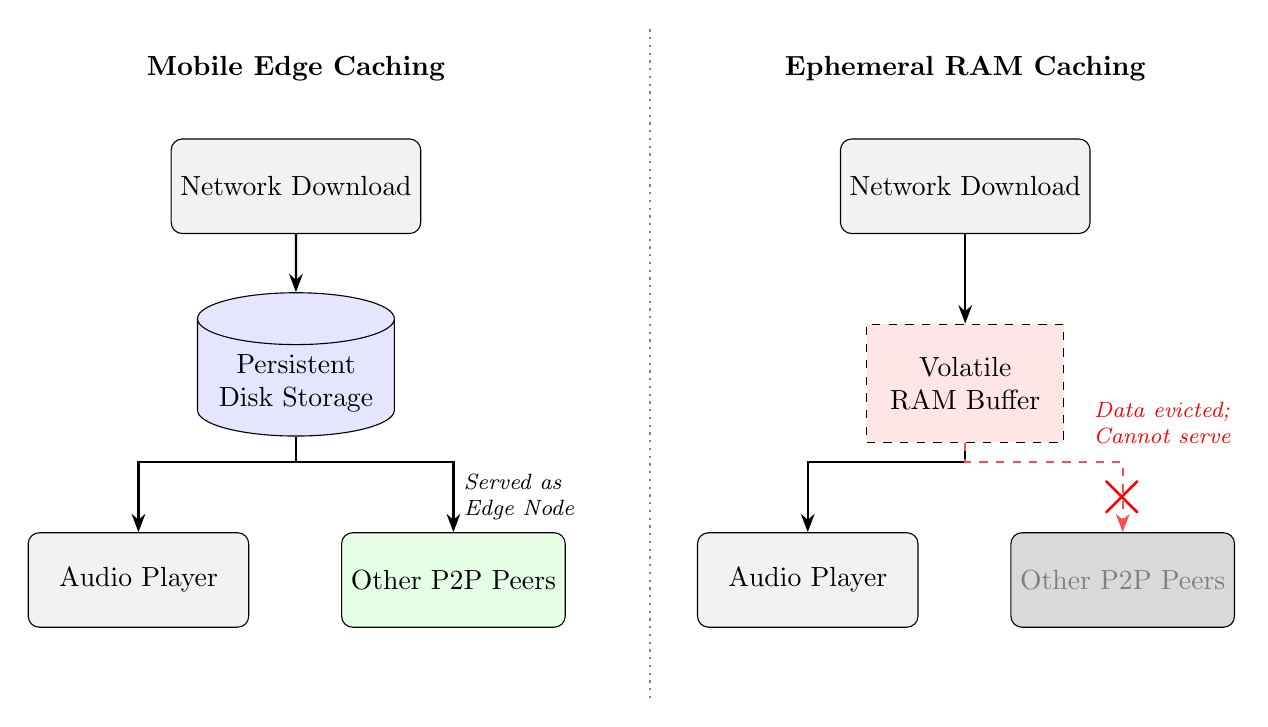
\begin{tikzpicture}[
        node distance=2cm,
        client/.style={draw, rectangle, minimum width=2.8cm, minimum height=1.2cm, align=center, fill=gray!10, rounded corners},
        storage/.style={draw, cylinder, aspect=0.3, minimum width=2.5cm, minimum height=1.5cm, align=center, fill=blue!10, shape border rotate=90},
        ram/.style={draw, rectangle, minimum width=2.5cm, minimum height=1.5cm, align=center, fill=red!10, dashed},
        arrow/.style={->, >=Stealth, thick}
    ]
        \node[font=\bfseries] (title_edge) at (0, 4.5) {Mobile Edge Caching};

        \node[client] (net_edge) at (0, 3) {Network Download};
        \node[storage] (disk) at (0, 0.5) {Persistent\\Disk Storage};

        \node[client] (play_edge) at (-2, -2) {Audio Player};
        \node[client, fill=green!10] (peer_edge) at (2, -2) {Other P2P Peers};

        \draw[arrow] (net_edge) -- (disk);

        \draw[arrow] (disk.south) -- (0, -0.5) -- (-2, -0.5) -- (play_edge.north);
        \draw[arrow] (disk.south) -- (0, -0.5) -- (2, -0.5) -- node[right, font=\footnotesize\itshape, align=left] {Served as\\Edge Node} (peer_edge.north);

        \node[font=\bfseries] (title_ram) at (8.5, 4.5) {Ephemeral RAM Caching};

        \node[client] (net_ram) at (8.5, 3) {Network Download};
        \node[ram] (ram_node) at (8.5, 0.5) {Volatile\\RAM Buffer};

        \node[client] (play_ram) at (6.5, -2) {Audio Player};
        \node[client, fill=gray!30, text=gray] (peer_ram) at (10.5, -2) {Other P2P Peers};

        \draw[arrow] (net_ram) -- (ram_node);

        \draw[arrow] (ram_node.south) -- (8.5, -0.5) -- (6.5, -0.5) -- (play_ram.north);
        \draw[arrow, dashed, draw=red!70] (ram_node.south) -- (8.5, -0.5) -- (10.5, -0.5) -- node[midway, text=red, font=\Huge\bfseries] {$\times$} (peer_ram.north);

        \node[font=\footnotesize\itshape, text=red, align=center] at (11, 0) {Data evicted;\\Cannot serve};

        \draw[thick, dotted, gray] (4.5, -3.5) -- (4.5, 5);

    \end{tikzpicture}
    \caption{Data flow comparison of Mobile Edge Caching vs Ephemeral RAM Caching.}
    \label{fig:storage_comparison}
\end{figure}

\section{Syncing and Integrity}
\indent \par The next decision is how the media file is structured during transfer. This choice determines how the file is segmented, exchanged, verified and recovered after failure. It also decides whether parallel downloading is possible at all. The two options considered here are chunk-based synchronization and continuous byte-stream transmission.


\subsection{Chunk-Based Synchronization}
\indent \par Under the chunk-based synchronization model, the complete file is deterministically split into small, fixed-size pieces. Data transfer and P2P exchange then happen at the granularity of these chunks. This approach provides strong data verification and fault tolerance, because each chunk has its own cryptographic checksum and only a corrupted chunk has to be downloaded again (see Figure \ref{fig:chunk_based_sync}). A good checksum for this verification is SHA-256, part of the NIST Secure Hash Standard, which makes the integrity rule independent of the peer that supplied the bytes \cite{secure_hash_standard}. The same structure enables parallel downloading: the client can request different chunks from multiple peers and increase total throughput. As established by Cohen's foundational BitTorrent architecture, distributing data in cryptographically verified pieces not only protects file integrity against malicious or faulty nodes, but also enables swarming, where a client downloads disjoint chunks from many independent sources \cite{bittorent}. This approach also facilitates deduplication, because the network can identify and share identical chunks across peers.

\begin{figure}[htbp]
    \centering
    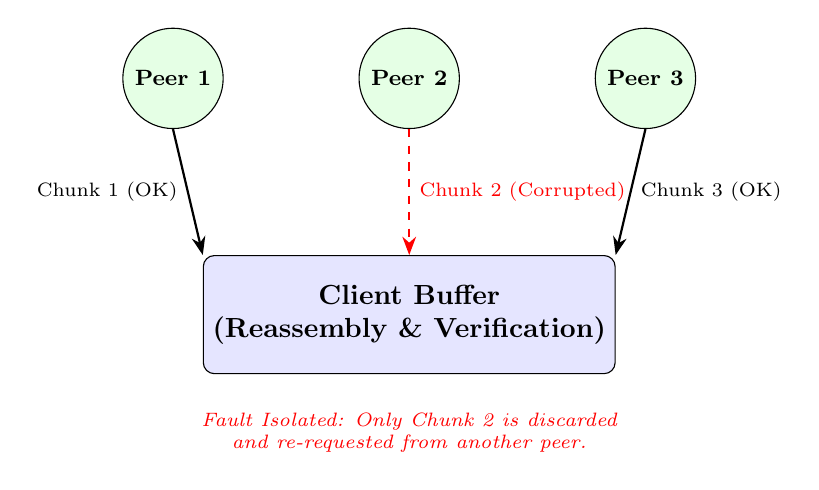
\begin{tikzpicture}[
        node distance=1.5cm,
        peer/.style={draw, circle, minimum size=1.2cm, align=center, fill=green!10, font=\footnotesize\bfseries},
        client/.style={draw, rectangle, minimum width=3cm, minimum height=1.5cm, align=center, fill=blue!10, rounded corners, font=\bfseries},
        arrow/.style={->, >=Stealth, thick},
        error_arrow/.style={->, >=Stealth, thick, dashed, draw=red},
        label_text/.style={font=\scriptsize\itshape, align=center, text=red}
    ]

        \node[peer] (peer1) at (0, 3) {Peer 1};
        \node[peer] (peer2) at (3, 3) {Peer 2};
        \node[peer] (peer3) at (6, 3) {Peer 3};
                \node[client] (client_chunk) at (3, 0) {Client Buffer\\(Reassembly \& Verification)};

        \draw[arrow] (peer1.south) -- node[left, font=\scriptsize] {Chunk 1 (OK)} (client_chunk.north west);
        \draw[error_arrow] (peer2.south) -- node[right, font=\scriptsize, align=left, text=red] {Chunk 2 (Corrupted)} (client_chunk.north);
        \draw[arrow] (peer3.south) -- node[right, font=\scriptsize] {Chunk 3 (OK)} (client_chunk.north east);

        \node[label_text] at (3, -1.5) {Fault Isolated: Only Chunk 2 is discarded\\and re-requested from another peer.};

    \end{tikzpicture}
    \caption{Chunk-Based Synchronization, corruption is isolated to individual segments.}
    \label{fig:chunk_based_sync}
\end{figure}

\par The cost is protocol overhead. Every chunk needs its own request and response, with transport headers and request identifiers. The client also has to maintain a real-time state map that tracks which chunks are downloaded, in transit or missing. Finally, the chunks must be reassembled in the correct order for gapless playback, which introduces strict buffer-management requirements at the application layer. As demonstrated by Zhang et al. in their data-driven P2P streaming network, this approach requires the active exchange of local 'Buffer Maps' between nodes and aggressive chunk scheduling so pieces arrive before their playback deadlines \cite{coolstreaming}.

\subsection{Continuous Byte-Stream}
\indent \par As an alternative, the continuous byte-stream approach treats the entire file as a single, contiguous pipe of data, mirroring traditional HTTP progressive streaming. The main advantage is low protocol overhead. Because the data is transmitted as a single continuous stream, the system avoids repetitive headers, request IDs and per-chunk checksums. The playback logic also becomes simpler, because the media player pulls data sequentially from a linear stream buffer without complex reordering.

\begin{figure}[htbp]
    \centering
    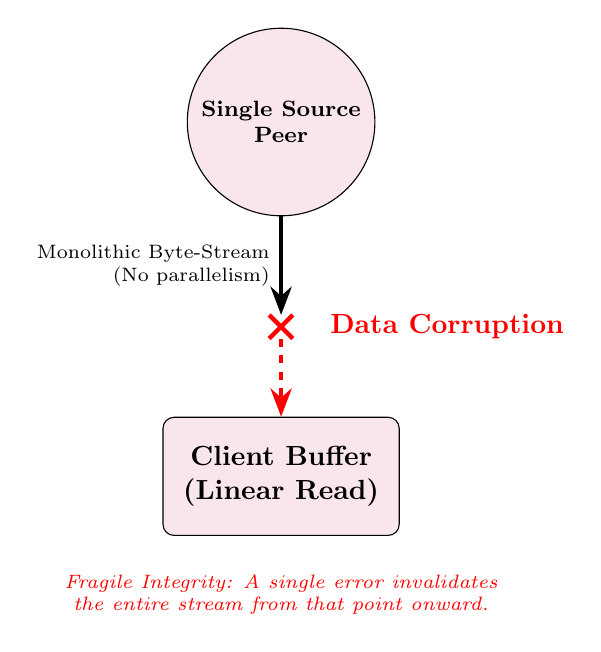
\begin{tikzpicture}[
        node distance=2cm,
        peer/.style={draw, circle, minimum size=1.5cm, align=center, fill=purple!10, font=\footnotesize\bfseries},
        client/.style={draw, rectangle, minimum width=3cm, minimum height=1.5cm, align=center, fill=purple!10, rounded corners, font=\bfseries},
        arrow/.style={->, >=Stealth, ultra thick},
        label_text/.style={font=\scriptsize\itshape, align=center, text=red}
    ]

        \node[peer] (peer_source) at (0, 4.5) {Single Source\\Peer};

        \node[client] (client_stream) at (0, 0) {Client Buffer\\(Linear Read)};

        \draw[arrow] (peer_source.south) -- node[pos=0.5, left, font=\scriptsize, align=right, text=black] {Monolithic Byte-Stream\\(No parallelism)} (0, 2.05);

        \draw[ultra thick, red] (-0.15, 2.05) -- (0.15, 1.75);
        \draw[ultra thick, red] (-0.15, 1.75) -- (0.15, 2.05);
        \node[font=\bfseries, text=red, right] at (0.5, 1.9) {Data Corruption};

        \draw[ultra thick, red, dashed, ->, >=Stealth] (0, 1.75) -- (client_stream.north);

        \node[label_text] at (0, -1.5) {Fragile Integrity: A single error invalidates\\the entire stream from that point onward.};

    \end{tikzpicture}
    \caption{Continuous Byte-Stream fragile single point of failure}
    \label{fig:continuous_stream_failure}
\end{figure}

\par Despite the simplicity, this method is incompatible with the core mechanics of a robust peer-assisted network. The monolithic structure prevents parallel downloading, because the client is effectively tied to one source at a time. More importantly, integrity becomes fragile (see Figure \ref{fig:continuous_stream_failure}). If one byte in the stream is corrupted or lost, the integrity of the file from that point onward is compromised. This is a realistic concern in a P2P system, where peer sessions can be short and unstable \cite{measurement_p2p}. Without granular checksums to isolate the error, the client may have to discard the received buffer and restart from a safe point, which is unacceptable for interactive playback.


\section{Managing Quality and Source Selection}
\indent \par Network conditions fluctuate constantly during streaming, so the distributed system needs a flow-control strategy. That strategy has to watch the current network conditions and decide how to avoid playback stalls. The two candidates differ in what they sacrifice when bandwidth drops: one lowers the quality of the audio, the other changes where the audio comes from. The two main options are adaptive bitrate and adaptive routing.

\subsection{Adaptive Bitrate}
\indent \par Adaptive Bitrate (ABR) dynamically changes the quality, and therefore the bitrate, of the content being streamed, based on the client's connection speed and buffer health. This approach is the established industry standard for centralised video streaming services such as YouTube and Netflix. As detailed by Stockhammer in the foundational specification of DASH (Dynamic Adaptive Streaming over HTTP), ABR breaks media into segments encoded at several bitrates, allowing the client to request the best representation for the current bandwidth \cite{standards_streaming_http}. HTTP Live Streaming follows the same family of ideas through variant streams that clients switch between based on network conditions \cite{hls_rfc8216}.


\par Its main advantage is playback continuity. By reducing the bitrate when bandwidth drops, the system lowers the chance of re-buffering and keeps the data rate close to the available network capacity. The stream therefore keeps flowing even on a degraded connection, where a fixed-quality stream would stall and re-buffer. The listener trades fidelity for the absence of interruptions, which is usually the right trade for video.

\par The drawback is that quality changes can be noticeable, especially in music if the representation switch affects perceived fidelity. From a provider perspective, ABR also complicates P2P sharing. The client has to manage a multidimensional chunk map that tracks both the chunk and its quality level, which makes peer discovery and deduplication much harder. The master server also has to compute and store multiple representations of every media file, increasing centralised storage cost. Figure \ref{fig:abr_fragmentation} illustrates the problem.

\begin{figure}[htbp]
    \centering
    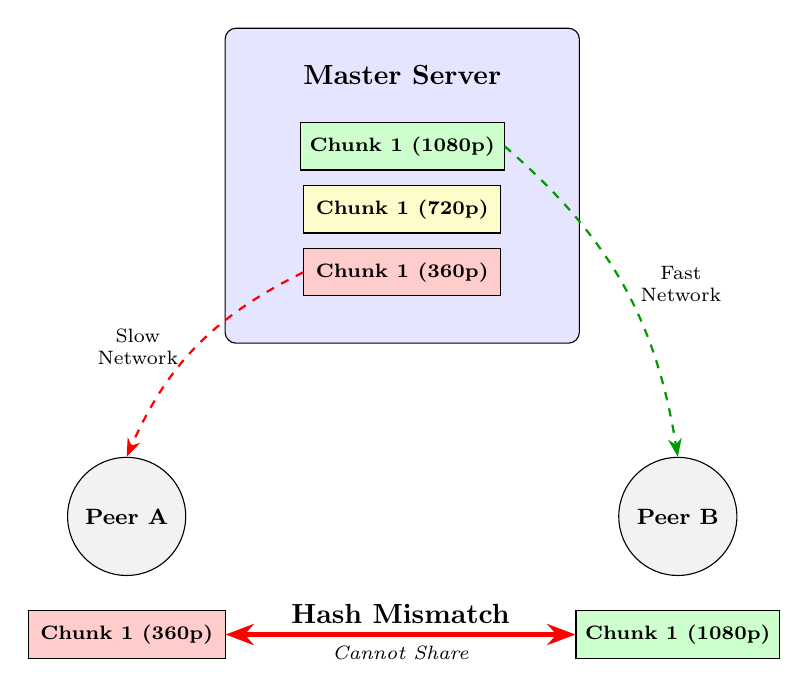
\begin{tikzpicture}[
        node distance=1.5cm,
        peer/.style={draw, circle, minimum size=1.5cm, align=center, fill=gray!10, font=\footnotesize\bfseries},
        chunk/.style={draw, rectangle, minimum width=2.5cm, minimum height=0.6cm, align=center, font=\scriptsize\bfseries},
        arrow/.style={->, >=Stealth, thick},
        label_text/.style={font=\scriptsize\itshape, align=center, text=red}
    ]

        \node[draw, rectangle, fill=blue!10, minimum width=4.5cm, minimum height=4cm, rounded corners] (server_box) at (0, 3.2) {};

        \node[align=center, font=\bfseries] (server_text) at (0, 4.6) {Master Server};

        \node[chunk, fill=green!20] (high) at (0, 3.7) {Chunk 1 (1080p)};
        \node[chunk, fill=yellow!20] (med) at (0, 2.9) {Chunk 1 (720p)};
        \node[chunk, fill=red!20] (low) at (0, 2.1) {Chunk 1 (360p)};

        \node[peer] (peer1) at (-3.5, -1) {Peer A};
        \node[peer] (peer2) at (3.5, -1) {Peer B};

        \node[chunk, fill=red!20] (peer1_chunk) at (-3.5, -2.5) {Chunk 1 (360p)};
        \node[chunk, fill=green!20] (peer2_chunk) at (3.5, -2.5) {Chunk 1 (1080p)};

        \draw[arrow, dashed, draw=red] (low.west) to[bend right=20] node[left, font=\scriptsize, align=center, xshift=-0.1cm] {Slow\\Network} (peer1.north);
        \draw[arrow, dashed, draw=green!60!black] (high.east) to[bend left=20] node[right, font=\scriptsize, align=center, xshift=0.1cm] {Fast\\Network} (peer2.north);

        \draw[<->, >=Stealth, ultra thick, draw=red] (peer1_chunk.east) -- node[above, font=\bfseries] {Hash Mismatch} node[below, font=\scriptsize\itshape] {Cannot Share} (peer2_chunk.west);

    \end{tikzpicture}
    \caption{Adaptive Bitrate example of failing peer-to-peer de-duplication.}
    \label{fig:abr_fragmentation}
\end{figure}

\subsection{Adaptive Routing}
\indent \par Alternatively, Adaptive Routing requires that the chosen quality remains strictly constant for the entire duration of the playback. If the current peer cannot sustain the required data flow, the system does not drop the quality, it immediately switches the download source. The client dynamically reroutes its chunk requests to a faster peer or, as an absolute last resort, falls back to the central Master Server to maintain the established bitrate (see Figure \ref{fig:adaptive_routing_switch}). The variable that absorbs network fluctuation is therefore the source of the bytes rather than their quality, which keeps the listening experience constant regardless of which peer happens to be supplying the audio at any given moment.

\par The most significant benefit of this approach is consistent quality. The user's experience is defined strictly by the fidelity they initially selected, maintaining client control regardless of network fluctuations. Architecturally, fixed-bitrate routing simplifies de-duplication and checksum verification. Because the quality is immutable, a specific chunk is mathematically identical across the entire P2P network, ensuring that cryptographic checksums always match and facilitating peer discovery logic.

\begin{figure}[htbp]
    \centering
    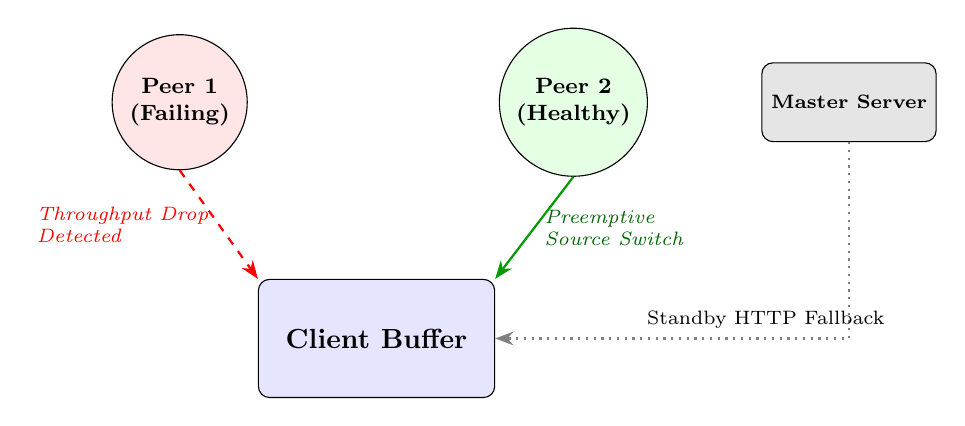
\begin{tikzpicture}[
        node distance=2cm,
        peer_red/.style={draw, circle, minimum size=1.5cm, align=center, fill=red!10, font=\footnotesize\bfseries},
        peer_green/.style={draw, circle, minimum size=1.5cm, align=center, fill=green!10, font=\footnotesize\bfseries},
        client/.style={draw, rectangle, minimum width=3cm, minimum height=1.5cm, align=center, fill=blue!10, rounded corners, font=\bfseries},
        arrow/.style={->, >=Stealth, thick},
        fail_arrow/.style={->, >=Stealth, thick, dashed, draw=red},
        label_text/.style={font=\scriptsize\itshape, align=left}
    ]
        \node[peer_red] (peer1) at (-2.5, 3) {Peer 1\\(Failing)};
        \node[peer_green] (peer2) at (2.5, 3) {Peer 2\\(Healthy)};
        \node[draw, rectangle, fill=gray!20, minimum width=2cm, minimum height=1cm, align=center, rounded corners, font=\scriptsize\bfseries] (server) at (6, 3) {Master Server};

        \node[client] (client_routing) at (0, 0) {Client Buffer};

        \draw[fail_arrow] (peer1.south) -- node[left, label_text, text=red] {Throughput Drop\\Detected} (client_routing.north west);
        \draw[arrow, draw=green!60!black] (peer2.south) -- node[right, label_text, text=green!40!black] {Preemptive\\Source Switch} (client_routing.north east);
        \draw[arrow, dotted, draw=gray] (server.south) |- node[above right, font=\scriptsize, pos=0.8] {Standby HTTP Fallback} (client_routing.east);

    \end{tikzpicture}
    \caption{Adaptive Routing data source switching.}
    \label{fig:adaptive_routing_switch}
\end{figure}

\par The cost of this strict quality rule is a higher risk of interruption. When a peer fails, the system has to switch sources quickly. If the routing switch takes too long, or if the replacement source also has insufficient bandwidth, playback stalls and the client has to re-buffer. As Magharei et al. demonstrated in their comparative study of P2P streaming architectures, maintaining continuous playback under these constraints requires a mesh-pull mechanism: the client must maintain a dynamic pool of standby neighbours and use aggressive chunk scheduling to request missing segments before the active playback buffer drains \cite{live_p2p_approaches}. The client therefore needs stricter buffer management and peer-performance prediction, and the central server still has to act as the final fail-safe when several peers fail at once.


\section{Lessons from Prior Peer-Assisted Systems}
\indent \par The five domains dissected above are not a checklist invented for this thesis. Every one of them was confronted, in some form, by the peer-assisted systems that came before it. Stepping back from the individual trade-offs to look at how complete systems combined them is instructive in two ways. It confirms that peer assistance is a proven technique rather than a speculative one, and it exposes precisely which of the older assumptions no longer hold under the browser, mobile and cloud constraints that this work targets.

\subsection{BitTorrent}
\indent \par The foundational reference point is BitTorrent, whose architecture Cohen described as a swarm of peers exchanging fixed-size, cryptographically identified pieces \cite{bittorent}. BitTorrent established the result that a population of downloaders can collectively serve a file with the origin contributing little more than the first complete copy, and that content-addressed pieces let a client assemble that file from many untrusted sources without sacrificing integrity. What it deliberately does not provide is any notion of a playback deadline: a torrent is finished when every piece has arrived, in whatever order, which is acceptable for a bulk download but not for a listener who expects sound the instant a track is clicked.

\subsection{CoolStreaming}
\indent \par CoolStreaming narrowed that gap for live media. Zhang et al. built a data-driven mesh in which peers periodically exchange 'buffer maps' advertising the segments they hold and pull missing segments from whichever partner can meet the playback deadline \cite{coolstreaming}. This demonstrated that a mesh-pull design can sustain media under real-time constraints, and it is the direct ancestor of the buffer-map peer discovery and deadline-aware chunk scheduling that reappear later in this thesis. Its assumptions, however, are those of live broadcast: a single shared timeline across all viewers, desktop clients on relatively stable connections, and a tolerance for several seconds of startup buffering that an on-demand music player cannot afford.

\subsection{Old Spotify}
\indent \par The closest precedent of all is Spotify's old production system. Kreitz and Niemel\"a measured a low-latency, peer-assisted music-on-demand architecture serving a large user base, in which the server delivered the beginning of each track and stood by as a fallback while peers supplied the remainder \cite{spotify_p2p}. The shape of that design, a server-seeded prefix, a peer swarm for the bulk of the bytes, and an origin fallback, is almost the same shape that the preceding sections kept arguing toward, which is reassuring: the architecture is known to work at scale. The follow-up work on integrating smartphones into the same model is equally instructive in the opposite direction, showing that mobile devices cannot be treated as desktop peers because battery state, radio access and aggressive background termination change what a peer can promise \cite{spotify_mobile_p2p}. Spotify ultimately retired its peer-assisted layer in favour of a pure cloud and CDN path, a decision driven less by any flaw in the model than by the operational simplicity of centralisation and the rise of the web client, which at the time had no way to open peer connections at all. The lesson this thesis takes from that history is that the model was never the problem, the platforms were, and the platform that made peer assistance impossible in the browser is precisely the one that WebRTC has since reopened.

\subsection{Hybrid CDN-P2P and Peer-Assisted CDNs}
\indent \par This reading is consistent with the broader academic treatment of the subject. Surveys of hybrid CDN-P2P and peer-assisted CDN architectures converge on the same division of labour, with the centralised infrastructure shrinking to a seeder and a guarantor of availability rather than the source of every byte \cite{hybrid_cdn_p2p,pa_cdn_survey}. On the cellular side, the device-to-device offloading literature frames the same exchange in terms of relieving network congestion at the cost of energy on the cooperating handset \cite{d2d_survey}, while long-running measurement studies of deployed peer populations supply the churn figures that any realistic cost estimate has to respect \cite{measurement_p2p}.


\indent \par Taken together, these systems establish two things that the rest of the thesis builds on. The origin is not eliminated but demoted, and the engineering problem is to make its role as small as the constraints allow. The five design choices are not independent knobs but a coupled system, in which a commitment in one domain closes options in the others. What the prior work does not supply is a single design that satisfies all five constraints simultaneously under modern conditions, and the instant-play expectation peculiar to music, together with a quantitative argument that the chosen design is the right one rather than merely a plausible one. Supplying that argument, and showing that the constraints leave essentially one coherent set of choices, is the work of the next chapter.

%\addcontentsline{toc}{chapter}{Introducere}
%\addcontentsline{toc}{chapter}{Introduction}

\chapter{Theoretical Background and Design Rationale}
\label{chap:ch2}

\tolerance=9999
\emergencystretch=3em

\par This chapter establishes the theoretical foundations on which the peer-assisted
streaming system rests, and justifies each major architectural decision in light of
those foundations.  The discussion proceeds from the broad landscape of content
delivery models, through the specifics of chunk-based media transport, peer
connectivity via WebRTC, and the prefix caching strategy, before arriving at a
formal bandwidth cost model that motivates the design as a whole.

% ─────────────────────────────────────────────────────────────────────────────
\section{Content Delivery Architecture Models}
\label{sec:delivery-models}

\par The way audio or video data travels from a content provider to a consumer has
evolved through several distinct architectural paradigms, each with a different
cost and latency profile.  Understanding these paradigms, and their respective
failure modes at scale, is a prerequisite for appreciating the design choices made
in this work.

\subsection{The Traditional Client-Server Model and its Cost Ceiling}
\label{subsec:client-server}

\par In the simplest delivery architecture, each client opens a direct TCP connection
to the origin server and streams data at the required bitrate.  The model is easy to
reason about: the server holds all content, all bandwidth is paid by the provider,
and clients are purely passive consumers.  The fundamental problem is that server
egress cost grows linearly with the number of concurrent listeners.  Formally, if a
song of size $S$ bytes is listened to by $N$ concurrent users, the total egress
volume is

\begin{equation}
  B_{\text{server}} = N \cdot S.
  \label{eq:server-cost}
\end{equation}

\par For large $N$, this is commercially unsustainable.  Cloud egress pricing from
major providers (AWS, GCP, Azure) is typically charged per gigabyte transferred out
of the data centre.  At a library of millions of tracks and tens of millions of daily
active users, equation~\eqref{eq:server-cost} translates directly into the
multi-hundred-million-dollar infrastructure bills observed at providers such as
Spotify \cite{spotify_google}.

\subsection{Content Delivery Networks}
\label{subsec:cdn}

\par Content Delivery Networks (CDNs) address the latency dimension of the
client-server problem by replicating popular content to geographically distributed
\emph{edge nodes}.  A client is routed to the nearest edge node, reducing the
round-trip time and often improving throughput.  However, CDNs do not reduce the
\emph{total} egress cost: every byte still originates from infrastructure owned or
leased by the provider and is billed at egress rates.  The replication itself
incurs additional intra-CDN transfer fees for warming edge caches.  Furthermore,
the replication model is poorly suited to long-tail content (rarely played tracks)
that must be stored at all edge locations despite being requested only occasionally.
CDNs therefore partially solve the latency problem while leaving the cost problem
intact.

\subsection{Peer-Assisted Hybrid Delivery}
\label{subsec:hybrid}

\par The peer-assisted model augments the client-server baseline with
device-to-device transfer.  After a client downloads a portion of content from the
server, it advertises that portion to other interested clients and serves it
directly over a P2P channel.  The server's role shifts from serving every byte to
serving only the initial fraction that bootstraps each new client into the swarm.
The theoretical minimum server egress for a swarm of $N$ users is achieved when
the first client downloads the full content from the server and every subsequent
client downloads entirely from peers:

\begin{equation}
  B_{\text{hybrid}}^{\min} = S + (N-1) \cdot \epsilon,
  \label{eq:hybrid-min}
\end{equation}

where $\epsilon$ is the per-client server overhead for bootstrapping (the prefix).
In practice, churn, clients leaving before peers can download from them, raises this
floor, but the gain over equation~\eqref{eq:server-cost} remains substantial even
under realistic churn rates.  Figure~\ref{fig:cost-comparison} illustrates the
asymptotic difference between the two models.

\begin{figure}[htbp]
\centering
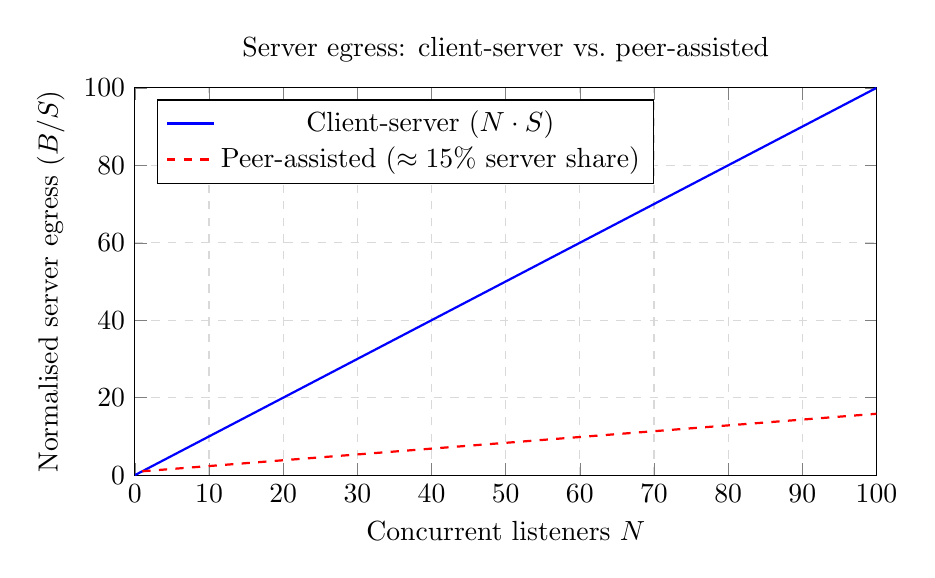
\begin{tikzpicture}
  \begin{axis}[
    width=11cm, height=6.5cm,
    xlabel={Concurrent listeners $N$},
    ylabel={Normalised server egress ($B / S$)},
    xmin=0, xmax=100,
    ymin=0, ymax=100,
    grid=both,
    grid style={dashed, gray!30},
    title={Server egress: client-server vs.\ peer-assisted},
    legend pos=north west,
  ]
    % Pure server: y = x
    \addplot[blue, thick, domain=0:100, samples=2]
      {x};
    \addlegendentry{Client-server ($N \cdot S$)}

    % Hybrid: y = 1 + (x-1)*0.15  (15% server fraction after bootstrap)
    \addplot[red, thick, dashed, domain=1:100, samples=100]
      {1 + (x-1)*0.15};
    \addlegendentry{Peer-assisted ($\approx 15\%$ server share)}
  \end{axis}
\end{tikzpicture}
\caption{Theoretical server egress volume as a function of concurrent listeners,
         contrasting pure client-server delivery with a peer-assisted model that
         routes 85\,\% of data through P2P channels.}
\label{fig:cost-comparison}
\end{figure}

\par The hybrid model introduces design constraints that the pure server model
avoids.  Peers must be discoverable, must hold relevant data at the right moment,
and must be reachable despite NAT and firewall boundaries.  The remainder of this
chapter addresses each of these constraints in turn.

% ─────────────────────────────────────────────────────────────────────────────
\section{Chunk-Based Streaming and Content-Addressed Storage}
\label{sec:chunk-theory}

\par The granularity at which content is partitioned has profound consequences for
both delivery efficiency and storage economy.  This section develops the theoretical
argument for fixed-size, content-addressed chunks as the primary storage and
transfer unit.

\subsection{Fixed-Size Partitioning}
\label{subsec:fixed-chunks}

\par Dividing an audio file into fixed-size blocks of $C$ bytes produces
$\lceil S / C \rceil$ chunks.  Fixed sizing, as opposed to variable-length
segmentation, has several practical advantages for a P2P system:

\begin{itemize}
  \item \textbf{Uniform scheduling}: a requester can ask any peer for ``chunk $i$''
        without needing to know the byte boundaries of that segment; the boundaries
        are implicit from $i \times C$.

  \item \textbf{Predictable buffer arithmetic}: the audio playback layer can
        translate byte-range requests into chunk indices with integer arithmetic,
        avoiding the need to transmit segment boundary tables.

  \item \textbf{Bounded memory}: a receiving buffer of fixed capacity (measured in
        chunks) is also bounded in bytes, enabling deterministic memory planning.
\end{itemize}

\par The choice of chunk size $C$ is a tuning parameter that trades latency for
overhead.  Smaller chunks reduce the time-to-first-byte of a P2P transfer but
increase the number of round trips and index entries.  Larger chunks amortise
per-request overhead but increase the granularity at which a peer can serve
partial data.  A size of $C = 65\,536$ bytes (64~KiB) sits at the intersection of
efficient I/O alignment (a power-of-two multiple of typical disk and network buffer
sizes) and practical P2P scheduling granularity.  At a typical audio bitrate of
320\,kbps for a high-quality MP3, one chunk holds approximately 1.6 seconds of
audio, giving a resolution that is finer than human perception of buffering
artefacts (${\sim}2{-}3$ seconds) while still being coarse enough to keep the
chunk count per song in the tens to low hundreds.

\subsection{Content-Addressed Storage and Deduplication}
\label{subsec:cas}

\par Content-addressed storage (CAS) is a paradigm in which the \emph{identity}
of a data block is derived from its \emph{content}, rather than from an externally
assigned identifier or file path.  The canonical mechanism is to use a
cryptographic hash of the block's bytes as its key.  This thesis uses SHA-256,
which maps any input to a 256-bit digest and has a collision probability of
approximately $2^{-256}$, negligible in any practical context.

\par The deduplication benefit of CAS is directly applicable to music libraries.
Many tracks share silence segments, common fade-outs, or identical album-art
headers embedded in audio containers.  With CAS, all such identical 64~KiB blocks
are stored once regardless of how many songs reference them.  More formally, if $k$
distinct byte-level 64~KiB blocks occur across all songs, the storage footprint is
$k \cdot C$ bytes, which is at most $\sum_i S_i$ (the sum of all song sizes) and
often substantially less.

\subsection{Hash-Based Integrity Verification}
\label{subsec:integrity}

\par The same SHA-256 digest that deduplicates storage also functions as an
integrity check.  Because the digest is precomputed at upload time and stored in
the chunk manifest, a client receiving chunk $i$ from \emph{any} source, origin
server or peer, can recompute the SHA-256 of the received bytes and compare it to
the expected value.  A mismatch unambiguously indicates corruption or deliberate
tampering.  This property is critical in the peer-assisted model, where a
misbehaving or compromised peer could otherwise inject corrupted audio data.  The
verification cost is negligible relative to network latency: a 64~KiB SHA-256
computation completes in under a microsecond on modern hardware \cite{sha256_perf}.

% ─────────────────────────────────────────────────────────────────────────────
\section{WebRTC as a Peer-to-Peer Transport Layer}
\label{sec:webrtc-theory}

\par Web Real-Time Communication (WebRTC) is an open standard that enables
browser and native applications to establish direct peer-to-peer connections
for audio, video, and arbitrary binary data, without requiring a dedicated relay
server for the media itself \cite{webrtc_spec}.  Its adoption in this system is
motivated by three properties: ubiquity (native support in all major browsers and
Flutter via the \texttt{flutter\_webrtc} package), NAT traversal capability, and
support for ordered reliable data channels.

\subsection{NAT Traversal: ICE, STUN, and TURN}
\label{subsec:nat-traversal}

\par The majority of end-user devices sit behind Network Address Translation (NAT)
gateways, which rewrite the source IP address and port of outgoing packets.  A
device behind NAT cannot be contacted directly by an external peer using its
private address; a traversal mechanism is required.

\par Interactive Connectivity Establishment (ICE) \cite{rfc8445} is the WebRTC
framework for discovering and negotiating a viable network path between two peers.
ICE collects \emph{candidates}, possible transport addresses, from three sources:

\begin{enumerate}
  \item \textbf{Host candidates}: the device's own network interface addresses.
  \item \textbf{Server-reflexive candidates}: the public IP/port mapping created
        by the NAT, discovered by querying a STUN (Session Traversal Utilities
        for NAT \cite{rfc8489}) server.
  \item \textbf{Relayed candidates}: addresses on a TURN (Traversal Using Relays
        around NAT \cite{rfc8656}) relay server, used only when direct
        connectivity fails.
\end{enumerate}

\par In most residential NAT configurations, a STUN exchange suffices: both peers
learn their server-reflexive addresses and use UDP hole-punching to establish a
direct path.  TURN relaying is reserved for symmetric NATs and enterprise
firewalls; its cost is significantly higher but its traffic volume is bounded
because the system falls back to server delivery rather than TURN when P2P fails.
Figure~\ref{fig:ice-flow} illustrates the ICE candidate exchange sequence.

\begin{figure}[htbp]
\centering
\resizebox{\textwidth}{!}{%
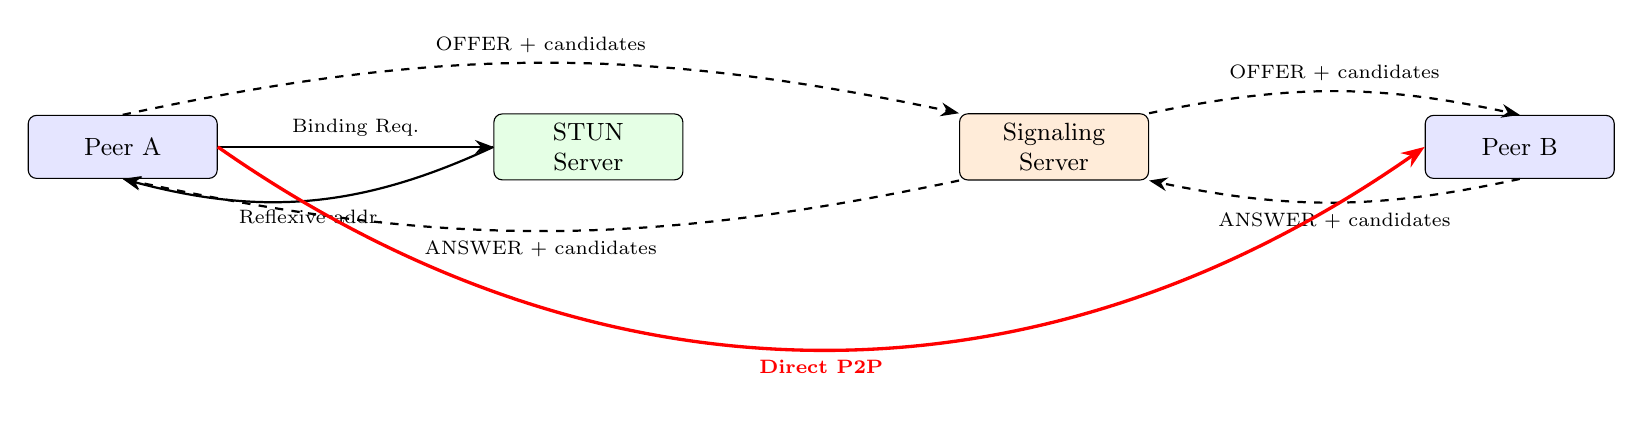
\begin{tikzpicture}[
  node distance=1.3cm and 3.5cm,
  box/.style={rectangle, draw, rounded corners=3pt,
              minimum width=2.4cm, minimum height=0.8cm,
              font=\small, align=center},
  srv/.style={box, fill=orange!15},
  peer/.style={box, fill=blue!10},
  stun/.style={box, fill=green!10},
  arr/.style={-{Stealth}, thick},
  darr/.style={-{Stealth}, thick, dashed}
]
  \node[peer]  (pA)   {Peer A};
  \node[stun, right=of pA]  (stun) {STUN\\Server};
  \node[srv,  right=of stun] (sig)  {Signaling\\Server};
  \node[peer, right=of sig]  (pB)   {Peer B};

  % STUN exchange
  \draw[arr]  (pA) -- node[above, font=\scriptsize]{Binding Req.} (stun);
  \draw[arr]  (stun.west) to[bend left=20]
              node[below, font=\scriptsize]{Reflexive addr.} (pA.south);

  % Candidate exchange via signaling
  \draw[darr] (pA.north) to[bend left=12]
              node[above, font=\scriptsize]{OFFER + candidates} (sig.north west);
  \draw[darr] (sig.north east) to[bend left=12]
              node[above, font=\scriptsize]{OFFER + candidates} (pB.north);
  \draw[darr] (pB.south) to[bend left=12]
              node[below, font=\scriptsize]{ANSWER + candidates} (sig.south east);
  \draw[darr] (sig.south west) to[bend left=12]
              node[below, font=\scriptsize]{ANSWER + candidates} (pA.south);

  % Direct P2P after ICE
  \draw[arr, red, very thick] (pA.east) to[bend right=35]
              node[below, font=\scriptsize, red]{\textbf{Direct P2P}} (pB.west);
\end{tikzpicture}%
}
\caption{ICE candidate exchange using a STUN server and signaling relay,
         resulting in a direct peer-to-peer data path.}
\label{fig:ice-flow}
\end{figure}

\subsection{Data Channels for Binary Chunk Transfer}
\label{subsec:data-channels}

\par WebRTC Data Channels provide an SCTP-over-DTLS transport that supports both
reliable ordered delivery (analogous to TCP) and unreliable unordered delivery
(analogous to UDP).  For audio chunk transfer, reliable ordered delivery is the
appropriate choice: audio data must arrive without corruption and the chunk
boundary semantics depend on receiving complete 64~KiB blocks.  Unlike TCP,
however, SCTP's head-of-line blocking is confined to a single stream, so a stalled
chunk request on one data channel does not block data channels to other peers.

\par The binary message format over a data channel is deliberately minimal.  A
fixed 8-byte header encodes the song identifier (4 bytes, big-endian) and the
chunk index (4 bytes, big-endian), followed directly by the audio payload.  The
choice of a fixed-length header over a framing protocol such as Protocol Buffers
is motivated by the fact that chunk transfers are entirely homogeneous, no
multiplexing of different message types is needed on a single data channel, so a
length-prefixed header would add overhead without benefit.

\subsection{Signaling and the Role of the Server}
\label{subsec:signaling-role}

\par WebRTC requires an \emph{out-of-band signaling channel} for the exchange of
SDP (Session Description Protocol) offer/answer payloads and ICE candidates.
This channel is the \emph{only} persistent server dependency in the P2P path; once
the data channel is open, the server is no longer involved in media transfer.  The
choice of WebSocket as the signaling transport aligns well with the existing server
infrastructure and allows the same connection to carry library synchronisation
events and peer discovery messages, reducing the number of persistent connections
each client must maintain.

% ─────────────────────────────────────────────────────────────────────────────
\section{The Prefix Caching Strategy}
\label{sec:prefix-theory}

\par A naive peer-assisted streaming system faces an irresolvable bootstrapping
problem: a new client cannot receive data from peers until it has connected to
them, and connecting to peers requires the ICE negotiation described in
Section~\ref{sec:webrtc-theory}, which takes hundreds of milliseconds.  During
this window, the audio player has no data to decode and playback cannot start.

\subsection{Playback Latency Decomposition}
\label{subsec:latency-decomp}

\par The total startup latency $T_{\text{start}}$ for a client requesting a song
can be decomposed as:

\begin{equation}
  T_{\text{start}} = T_{\text{resolve}} + T_{\text{buffer}},
  \label{eq:latency}
\end{equation}

where $T_{\text{resolve}}$ is the time to acquire enough data for the audio decoder
to begin, and $T_{\text{buffer}}$ is the time to buffer a sufficient lookahead to
avoid starvation during subsequent streaming.  In the P2P model, $T_{\text{resolve}}$
is dominated by the WebRTC connection setup time ($T_{\text{ICE}} \approx
200{-}500$\,ms) plus the first chunk transfer latency.  An unmitigated peer-first
strategy would therefore introduce a mandatory 200–500 ms delay even for popular
songs with many available peers.

\par The prefix strategy eliminates this delay by decoupling the initial buffer fill
from peer discovery.  The client simultaneously (a) fetches a fixed prefix of the
song from the origin server over HTTP and (b) initiates peer discovery via the
signaling server.  Playback begins as soon as the prefix arrives; by the time the
prefix is consumed, peer connections are typically established and the remainder
of the song is served from peers.

\subsection{Choosing the Prefix Threshold}
\label{subsec:prefix-threshold}

\par The prefix must be large enough that $T_{\text{buffer}}$ covers the full peer
negotiation time $T_{\text{ICE}}$ plus the first peer response time.  Let $r$ be
the audio bitrate in bytes per second and $P$ be the prefix size in bytes.  The
prefix sustains playback for $P / r$ seconds.  For this to cover ICE negotiation
and an initial P2P timeout of $T_{\text{p2p}}$ seconds, we require:

\begin{equation}
  \frac{P}{r} > T_{\text{ICE}} + T_{\text{p2p}}.
  \label{eq:prefix-condition}
\end{equation}

\par At $r = 40\,960$ bytes/s (320\,kbps), $T_{\text{ICE}} = 500$\,ms, and
$T_{\text{p2p}} = 1000$\,ms, equation~\eqref{eq:prefix-condition} gives
$P > 61\,440$ bytes, less than one chunk.  The chosen prefix of eight chunks
(524\,288 bytes, sustaining $\approx 12.8$\,s of playback) provides a generous
safety margin that accommodates slow NAT environments, CDN cold-starts on the
server prefix fetch, and the 16-chunk lookahead prefetch window.  The same eight
chunks are used as the boundary below which the client unconditionally fetches
from the server, aligning the prefix delivery endpoint with the P2P onset point
and making the server's prefix endpoint a natural cache target.

\subsection{Proactive Queue Prefetching}
\label{subsec:proactive-theory}

\par A user listening to a playlist will transition between songs with negligible
delay only if the next song's startup sequence (prefix fetch and peer negotiation)
completes before the current song ends.  Proactive prefetching addresses this by
initiating prefix downloads for the next $k$ songs in the queue while the current
song is playing.  The bandwidth overhead is bounded: the total proactive download
is $k \cdot P$ bytes, which for $k = 5$ and $P = 524\,288$ bytes totals
approximately 2.5~MiB, a modest background cost compared to the elimination of any
inter-song latency.

% ─────────────────────────────────────────────────────────────────────────────
\section{Bandwidth Cost Model}
\label{sec:cost-model}

\par Having established the individual mechanisms, this section synthesises them
into a formal cost model that quantifies the expected reduction in server egress
and motivates the specific parameter choices made in the implementation.

\subsection{Theoretical Offload Ratio}
\label{subsec:offload-ratio}

\par Define the \emph{offload ratio} $\rho$ as the fraction of total bytes served
by peers rather than the origin server.  For a swarm of $N$ simultaneous listeners
of a song of size $S$, each listener requires one prefix of size $P$ from the
server.  Assuming all non-prefix bytes are served by peers (the ideal case), the
server egress is $N \cdot P$ and the total bytes consumed is $N \cdot S$:

\begin{equation}
  \rho = 1 - \frac{P}{S} = 1 - \frac{8C}{S},
  \label{eq:offload-ratio}
\end{equation}

where $C = 65\,536$ bytes.  For a 4-minute song at 320\,kbps, $S \approx 9.6$\,MB
and $8C \approx 0.52$\,MB, giving $\rho \approx 94.6\,\%$.  Even a 1-minute track
($S \approx 2.4$\,MB) yields $\rho \approx 78.3\,\%$.  These figures represent
upper bounds; in practice, churn and cold starts reduce the achievable ratio, but
the asymptotic behaviour in equation~\eqref{eq:server-cost} is converted from
$O(N)$ to $O(1)$ in server egress per unit time, the cost becomes independent of
swarm size.

\subsection{Design Trade-offs and Parameter Sensitivity}
\label{subsec:tradeoffs}

\par The model reveals several trade-offs that informed the implementation:

\begin{itemize}
  \item \textbf{Prefix size vs.\ offload ratio}: A larger prefix reduces $\rho$
        (more server cost) but increases startup robustness.  The chosen eight
        chunks balance these concerns, as shown by equation~\eqref{eq:prefix-condition}.

  \item \textbf{P2P timeout vs.\ stall probability}: A longer timeout gives slow
        peers more time to respond, increasing the offload ratio, but risks
        audible stalls if the audio player exhausts its lookahead buffer.  The
        one-second timeout, combined with a 16-chunk ($\approx 1$\,MB) lookahead,
        ensures the buffer survives one failed peer request before the server
        fallback path returns data.

  \item \textbf{Chunk size vs.\ overhead}: Halving $C$ to 32~KiB would double
        the chunk count and index size while reducing the per-chunk transfer
        latency.  Doubling $C$ to 128~KiB would reduce overhead but coarsen
        the P2P scheduling granularity, making it harder for a peer to serve
        partial data if it has only downloaded part of a large block.  The
        64~KiB value sits at a practical optimum for the target content
        (320\,kbps MP3 and FLAC).

  \item \textbf{Swarm size and peer density}: The model assumes at least one
        peer with a given chunk is reachable within the P2P timeout.  For
        long-tail songs with very few listeners, peers may be absent and the
        system degrades gracefully to pure server delivery.  No additional
        logic or user experience penalty is incurred in this case: the
        server fallback is always available and the one-second timeout is
        the only overhead.
\end{itemize}

\par Table~\ref{tab:param-summary} summarises the key parameters and their
theoretical justification.

\begin{table}[htbp]
\centering
\begin{tabular}{|p{3.8cm}|p{2.2cm}|p{7.5cm}|}
\hline
\textbf{Parameter} & \textbf{Value} & \textbf{Justification} \\
\hline
Chunk size $C$ & 65\,536 B & Power-of-two I/O alignment; $\approx 1.6$\,s of 320\,kbps audio \\
\hline
Prefix chunks & 8 & Covers $T_{\text{ICE}} + T_{\text{p2p}}$ at max audio bitrate with safety margin \\
\hline
P2P timeout & 1\,000\,ms & Balances peer-wait cost against 16-chunk buffer capacity \\
\hline
Lookahead & 16 chunks & $\approx 1$\,MiB; absorbs one full P2P timeout without stall \\
\hline
RAM cache size & 15 chunks & Absorbs overlapping range requests from audio player \\
\hline
Proactive prefetch & 5 songs & Eliminates inter-song latency; adds $\approx 2.5$\,MiB background load \\
\hline
State save interval & 30\,s & Limits server write load while bounding session data loss \\
\hline
\end{tabular}
\caption{Key system parameters and their theoretical justification.}
\label{tab:param-summary}
\end{table}

\chapter{System Implementation}
\label{chap:ch3}

\tolerance=9999
\emergencystretch=3em

\par This chapter presents the concrete implementation of the peer-assisted music streaming system,
describing how the architectural concepts introduced in the previous chapter are realised in code.
The discussion proceeds from the data model and server-side components through to the client-side
streaming pipeline, and concludes with a set of annotated flow diagrams that highlight the
decision-making logic embedded in each major subsystem.

% ─────────────────────────────────────────────────────────────────────────────
\section{Backend Data Model and Storage Layer}
\label{sec:data-model}

\par The persistence layer is built on PostgreSQL and managed through Liquibase changesets,
keeping the schema under version control and decoupled from the JPA entity definitions.
The JPA DDL mode is set to \texttt{validate-only}, so every structural change must be
expressed as a new changeset rather than relying on automatic schema generation.

\subsection{Content-Addressed Chunk Storage}
\label{subsec:chunk-storage}

\par The central design decision for audio storage is to decompose each song into fixed-size
\emph{chunks} of exactly 65\,536 bytes (64~KiB) and to store them independently.
Each chunk is represented by the \texttt{Chunk} entity, whose most important field is
\texttt{contentHash}, a 256-bit SHA-256 digest of the raw audio bytes.
The hash serves a dual purpose: it acts as a natural deduplication key, so that two songs
sharing an identical segment only ever store one physical file, and it provides an integrity
fingerprint that both server and client can verify before using the data.

\par The \texttt{storagePath} field records the filesystem location of the corresponding file,
and the \texttt{size} field caches the byte count for range-request arithmetic.
The \texttt{SongChunk} join entity binds a \texttt{Song} to its constituent \texttt{Chunk}
objects via an ordered \texttt{orderIndex} column, preserving the sequential structure of the
audio file.  The relationship is illustrated in Figure~\ref{fig:chunk-model}.

\begin{figure}[htbp]
\centering
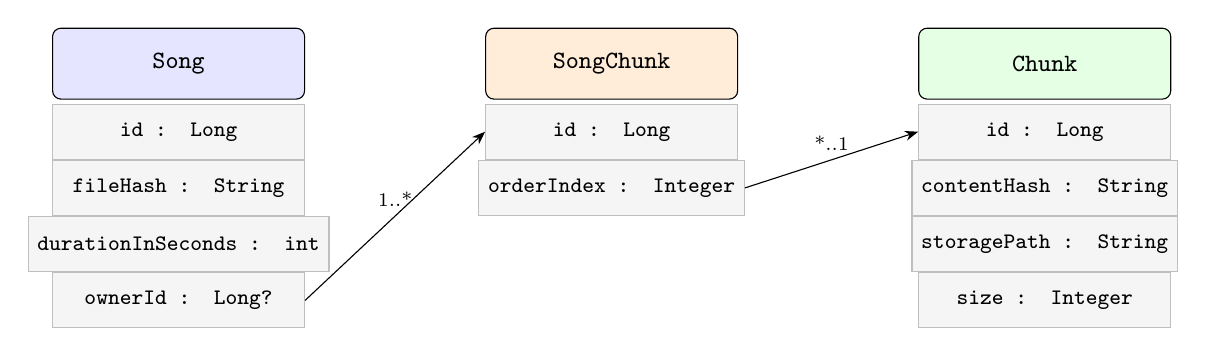
\begin{tikzpicture}[
    entity/.style={rectangle, draw, rounded corners=3pt,
                   minimum width=3.2cm, minimum height=0.9cm,
                   font=\small\ttfamily},
    field/.style={rectangle, draw=gray!50, minimum width=3.2cm,
                  minimum height=0.7cm, font=\footnotesize\ttfamily,
                  fill=gray!8},
    lbl/.style={font=\scriptsize, midway, above}
]
  % Song
  \node[entity, fill=blue!10] (song) at (0,0) {Song};
  \node[field, below=0pt of song, yshift=-0.05cm] (s1) {id : Long};
  \node[field, below=0pt of s1] (s2) {fileHash : String};
  \node[field, below=0pt of s2] (s3) {durationInSeconds : int};
  \node[field, below=0pt of s3] (s4) {ownerId : Long?};

  % SongChunk
  \node[entity, fill=orange!15] (sc) at (5.5,0) {SongChunk};
  \node[field, below=0pt of sc, yshift=-0.05cm] (c1) {id : Long};
  \node[field, below=0pt of c1] (c2) {orderIndex : Integer};

  % Chunk
  \node[entity, fill=green!10] (ch) at (11,0) {Chunk};
  \node[field, below=0pt of ch, yshift=-0.05cm] (ch1) {id : Long};
  \node[field, below=0pt of ch1] (ch2) {contentHash : String};
  \node[field, below=0pt of ch2] (ch3) {storagePath : String};
  \node[field, below=0pt of ch3] (ch4) {size : Integer};

  % Arrows
  \draw[-{Stealth}] (s4.east) -- node[above, font=\scriptsize]{1..*} (c1.west);
  \draw[-{Stealth}] (c2.east) -- node[above, font=\scriptsize]{*..1} (ch1.west);
\end{tikzpicture}
\caption{Simplified entity relationship between \texttt{Song}, \texttt{SongChunk}, and \texttt{Chunk}.}
\label{fig:chunk-model}
\end{figure}

\par Because chunks are content-addressed, the upload pipeline hashes each 64~KiB block
before writing it to disk.  If an identical hash already exists in the database the physical
file is reused and only a new \texttt{SongChunk} row is inserted.  This strategy is
particularly effective for music libraries where intros, outros, and silence segments repeat
across many tracks.

\subsection{User Library and Soft Deletion}
\label{subsec:user-library}

\par Each user's relationship to a song is captured by the \texttt{UserLibrary} entity, which
uses a composite primary key of \texttt{(userId, songId)}.  Engagement fields---\texttt{liked},
\texttt{playCount}, \texttt{lastPlayed}, and \texttt{addedAt}---are stored alongside a
\texttt{lastUpdated} timestamp that drives the incremental synchronisation protocol described
in Section~\ref{sec:data-sync}.  Deletion is implemented as a soft flag (\texttt{isDeleted})
so that the sync engine can propagate removal events to other devices without losing the
record itself.

\par The \texttt{ownerId} field on \texttt{Song} distinguishes between platform-owned catalogue
tracks (nullable owner) and user-uploaded files (set owner).  The streaming service enforces
this at the query level: requests for user-uploaded songs are rejected if the authenticated
user does not match \texttt{ownerId}, providing simple but effective access control.

% ─────────────────────────────────────────────────────────────────────────────
\section{Server-Side Streaming Service}
\label{sec:streaming-service}

\par The \texttt{StreamingService} exposes three retrieval modes to REST clients: a manifest
endpoint, a per-chunk endpoint, and a prefix endpoint.  All three are generated from the
OpenAPI specification in \texttt{api.yml}; the service class implements the generated
controller interface and contains the business logic.

\subsection{Chunk Manifest}
\label{subsec:manifest}

\par Before a client can stream a song it fetches the \emph{chunk manifest}: a lightweight
JSON document that describes the song's chunk count, individual chunk size, total byte length,
and, critically, an ordered list of SHA-256 hashes, one per chunk.
The manifest allows the client to verify every chunk it receives regardless of whether that
chunk arrived from the origin server or from a peer.  Generating the manifest requires a single
database join (\texttt{Song} $\rightarrow$ \texttt{SongChunk} $\rightarrow$ \texttt{Chunk})
ordered by \texttt{orderIndex}, after which the service projects the \texttt{contentHash}
fields into the response DTO.

\subsection{Prefix Delivery}
\label{subsec:prefix}

\par To guarantee that playback can begin immediately (before any peer connection is
established) the server supports a \emph{prefix endpoint} that returns the first
$N$ bytes of a song as a single binary response.  The default prefix size is
512\,000 bytes (approximately 500~KiB), which corresponds to the first eight 64~KiB chunks.
The implementation iterates through the ordered \texttt{SongChunk} list, opens each
chunk file, appends bytes to a buffer, and returns once the \texttt{bytesNeeded}
threshold is reached.  The choice of eight chunks as the prefix boundary is not
arbitrary: it is exactly the threshold used by the client-side \texttt{ChunkService}
to decide whether to attempt a peer fetch, ensuring that the server-delivered prefix
and the subsequent peer-assisted stream are seamlessly contiguous.

\subsection{Per-Chunk and Full-Stream Endpoints}
\label{subsec:per-chunk}

\par Individual chunk retrieval (\texttt{getSongChunk}) simply looks up the
\texttt{SongChunk} for the requested \texttt{(songId, chunkIndex)} pair, opens the
physical file at \texttt{storagePath}, and returns the raw bytes.
The full-stream endpoint assembles a \texttt{SequenceInputStream} over all chunk
files and is provided as a compatibility fallback for clients that cannot support
the chunked protocol, for example certain browser-embedded players.

% ─────────────────────────────────────────────────────────────────────────────
\section{Peer Registry with Redis}
\label{sec:peer-registry}

\par The server must know, at the moment a client requests peer discovery, which
other clients hold which chunks.  This state is ephemeral (it exists only while
clients are connected) and must be shared across multiple server instances in a
horizontally-scaled deployment.  Redis was chosen for this purpose because it
provides the required atomicity primitives (hash operations, set operations) with
sub-millisecond latency.

\par The \texttt{PeerTrackingService} maintains two data structures in Redis for
each active peer:

\begin{itemize}
  \item \textbf{Chunk index}: a Redis \emph{hash} keyed as \texttt{peer:chunks:\{songId\}},
        mapping each peer identifier to a JSON-serialised \texttt{Set<Integer>} of chunk
        indices that the peer has locally cached.
  \item \textbf{Song index}: a Redis \emph{set} keyed as \texttt{peer:songs:\{peerId\}},
        recording which song IDs the peer has registered chunks for.  This reverse
        index enables efficient cleanup on disconnection.
\end{itemize}

\par When a peer announces a new set of cached chunks (message type
\texttt{REGISTER\_CACHE}), the service fetches the existing entry for that
\texttt{(songId, peerId)} pair, computes the union with the incoming indices,
and writes the result back.  This incremental merge avoids requiring peers to
retransmit their full cache state on every update.

\par On disconnection, \texttt{unregisterPeer} iterates the song index to enumerate
every song the peer had cached, removes the peer's entry from each chunk hash, and
then deletes the song index itself, leaving no stale entries in Redis.

% ─────────────────────────────────────────────────────────────────────────────
\section{WebSocket Signaling Server}
\label{sec:signaling}

\par WebRTC connections between clients require out-of-band signaling to exchange
Session Description Protocol (SDP) offers and answers as well as Interactive
Connectivity Establishment (ICE) candidates.  The \texttt{SignalingHandler}
implements the Spring \texttt{TextWebSocketHandler} interface and acts as this
signaling relay, while also serving as the delivery channel for server-initiated
events such as synchronisation triggers and playback state changes.

\subsection{Connection State}
\label{subsec:conn-state}

\par The handler maintains three in-memory concurrent maps:

\begin{itemize}
  \item \texttt{registry}: maps each WebSocket session ID to a \texttt{ClientConnection}
        record, which bundles the \texttt{WebSocketSession}, the peer identifier, and the optional authenticated user ID.
  \item \texttt{userIndex}: maps each user ID to the set of session IDs belonging to
        that user, allowing server events to fan out to all of a user's connected devices.
  \item \texttt{peerIndex}: maps each peer identifier to its session ID, enabling direct
        routing when the target peer is hosted by this server instance.
\end{itemize}

\par When a new connection arrives, a preliminary \texttt{ClientConnection} is created with placeholder identifiers.  The first incoming message that carries a \texttt{senderId} and \texttt{userId} promotes the connection to a fully identified state, populating both indexes.

\subsection{Message Routing}
\label{subsec:msg-routing}

\par The five message types the handler processes are:

\begin{itemize}
  \item \textbf{\texttt{REGISTER\_CACHE}}: Delivered by a peer after it has cached one
        or more chunks.  The payload is a set of integer chunk indices.  The handler
        delegates to \texttt{PeerTrackingService.register\-PeerChunks}.

  \item \textbf{\texttt{DISCOVER\_PEERS}}: A request for the chunk maps of all other
        peers that hold data for a given song.  The handler calls
        \texttt{PeerTrackingService.getPeer\-BufferMapsForSong}, filters out the
        requesting peer's own entry, and replies with a \texttt{PEER\_BUFFER\_MAP} message.

  \item \textbf{\texttt{OFFER} / \texttt{ANSWER} / \texttt{ICE\_CANDIDATE}}: WebRTC
        signaling messages that carry a \texttt{targetId} field.  The handler attempts to
        route the message to the target peer locally via \texttt{peerIndex}; if the target
        session is not present on this instance, the message is published to the Redis
        \texttt{signaling:webrtc} channel so that a \texttt{RedisSignaling\-Listener}
        on another instance can deliver it.
\end{itemize}

\par The Redis pub/sub bridge is what enables horizontal scaling: each server instance runs a \texttt{RedisSignalingListener} that subscribes to three channels: 
\texttt{signaling:webrtc}, \texttt{signaling:sync}, and \texttt{signaling:playback},
and delivers arriving messages to the locally connected sessions they target.
Figure~\ref{fig:signaling-flow} illustrates the cross-instance routing path.

\begin{figure}[htbp]
\centering
\resizebox{\textwidth}{!}{%
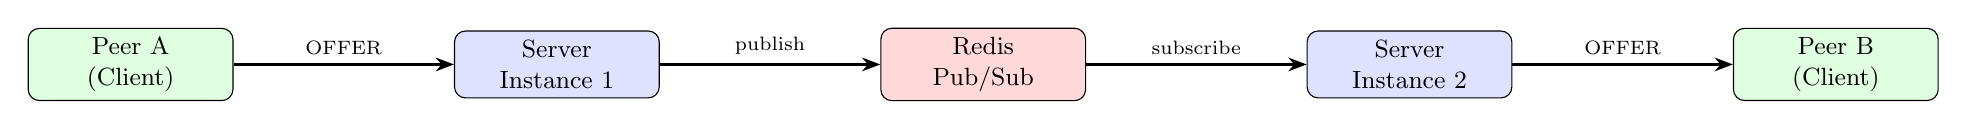
\begin{tikzpicture}[
  node distance=1.4cm and 2.8cm,
  box/.style={rectangle, draw, rounded corners=4pt,
              minimum width=2.6cm, minimum height=0.85cm,
              font=\small, align=center},
  redis/.style={box, fill=red!15},
  srv/.style={box, fill=blue!12},
  cli/.style={box, fill=green!12},
  arr/.style={-{Stealth}, thick}
]
  \node[cli]  (peerA) {Peer A\\(Client)};
  \node[srv, right=of peerA] (srv1) {Server\\Instance 1};
  \node[redis, right=of srv1] (redis) {Redis\\Pub/Sub};
  \node[srv, right=of redis] (srv2) {Server\\Instance 2};
  \node[cli, right=of srv2] (peerB) {Peer B\\(Client)};

  \draw[arr] (peerA) -- node[above, font=\scriptsize]{OFFER} (srv1);
  \draw[arr] (srv1)  -- node[above, font=\scriptsize]{publish} (redis);
  \draw[arr] (redis) -- node[above, font=\scriptsize]{subscribe} (srv2);
  \draw[arr] (srv2)  -- node[above, font=\scriptsize]{OFFER} (peerB);
\end{tikzpicture}%
}
\caption{Cross-instance WebRTC signal routing via Redis pub/sub.}
\label{fig:signaling-flow}
\end{figure}

% ─────────────────────────────────────────────────────────────────────────────
\section{Data Synchronisation Service}
\label{sec:data-sync}

\par The \texttt{DataSyncService} implements a bidirectional, timestamp-based
synchronisation protocol that keeps the user's library consistent across devices
without requiring a full reload of the catalogue.

\par A client sends a \texttt{SyncRequestDto} containing an optional
\texttt{lastSyncTime} ISO-8601 timestamp and a list of \texttt{localChanges}: each
a \texttt{SongSyncDto} encoding a song's updated engagement fields (\texttt{liked},
\texttt{playCountDelta}, \texttt{lastPlayed}, \texttt{isDeleted}).  The service
applies these changes to the corresponding \texttt{UserLibrary} rows inside a single
transaction, then queries for all \texttt{UserLibrary} entries with
\texttt{lastUpdated > lastSyncTime} to collect server-side changes.
The response carries both sets of changes and a new \texttt{syncTimestamp} that the
client stores locally for use in the next synchronisation call.

\par After the write phase completes, the service invokes
\texttt{SignalingHandler.sendSyncTrigger(userId)}, publishing a notification to the
Redis \texttt{signaling:sync} channel.  All other devices belonging to the same user
receive this trigger via the pub/sub bridge and initiate their own sync request,
propagating library changes across devices in near real time.

% ─────────────────────────────────────────────────────────────────────────────
\section{Client-Side Chunk Retrieval}
\label{sec:chunk-service}

\par On the client the \texttt{ChunkService} class encapsulates the full logic for
obtaining a single chunk, regardless of whether that chunk originates from the server, a peer, or a local cache.  Each \texttt{ChunkService} instance is bound to one song and is created by \texttt{AppAudioService} the first time a song is queued for playback.

\subsection{Caching Architecture}
\label{subsec:caching}

\par Three caching layers are stacked in order of access speed:

\begin{enumerate}
  \item \textbf{Hot RAM cache}: a map of at most 15 entries keyed by chunk index.
        Entries are evicted using a least-recently-used policy when the map exceeds
        capacity.  This layer absorbs repeated reads for the same chunk that occur
        when the audio player issues overlapping range requests.

  \item \textbf{Disk cache}: a \texttt{ChunkCacheRepository} that stores chunks as
        binary files under a per-song directory.  Writes are asynchronous; the chunk
        is placed in the RAM cache first and persisted in the background.

  \item \textbf{Active request deduplication}: a map from chunk index to a
        \texttt{Future<Uint8List>}.  If two callers concurrently request the same chunk,
        the second caller attaches to the existing future rather than issuing a duplicate
        network or peer request.
\end{enumerate}

\subsection{Fetch Decision Logic}
\label{subsec:fetch-logic}

\par The core method \texttt{\_fetchChunkLogic(int index)} implements a three-branch
decision tree, illustrated in Figure~\ref{fig:chunk-fetch-flow}:

\begin{enumerate}
  \item If $\texttt{index} < 8$, the chunk belongs to the \emph{server prefix} and
        is always fetched from the origin server.  This guarantees that playback can
        begin while peer connections are still being negotiated.

  \item Otherwise, if at least one peer with the requested chunk index is known,
        a P2P request is issued through \texttt{WebRTCService} with a timeout of
        one second.  If the peer responds in time, the data is integrity-verified
        against the SHA-256 hash from the manifest.  A verification failure causes
        an immediate fallback to the server, and if the server copy also fails
        verification, a \texttt{ChunkIntegrityException} is thrown to halt playback.

  \item If no suitable peer exists, or if the peer request times out, the chunk is
        fetched from the origin server.
\end{enumerate}

\par Every successfully fetched chunk is written to both the disk cache and the RAM
cache, and the peer registry is updated via a \texttt{REGISTER\_CACHE} WebSocket
message so that other peers can subsequently discover this device as a source.

\begin{figure}[htbp]
\centering
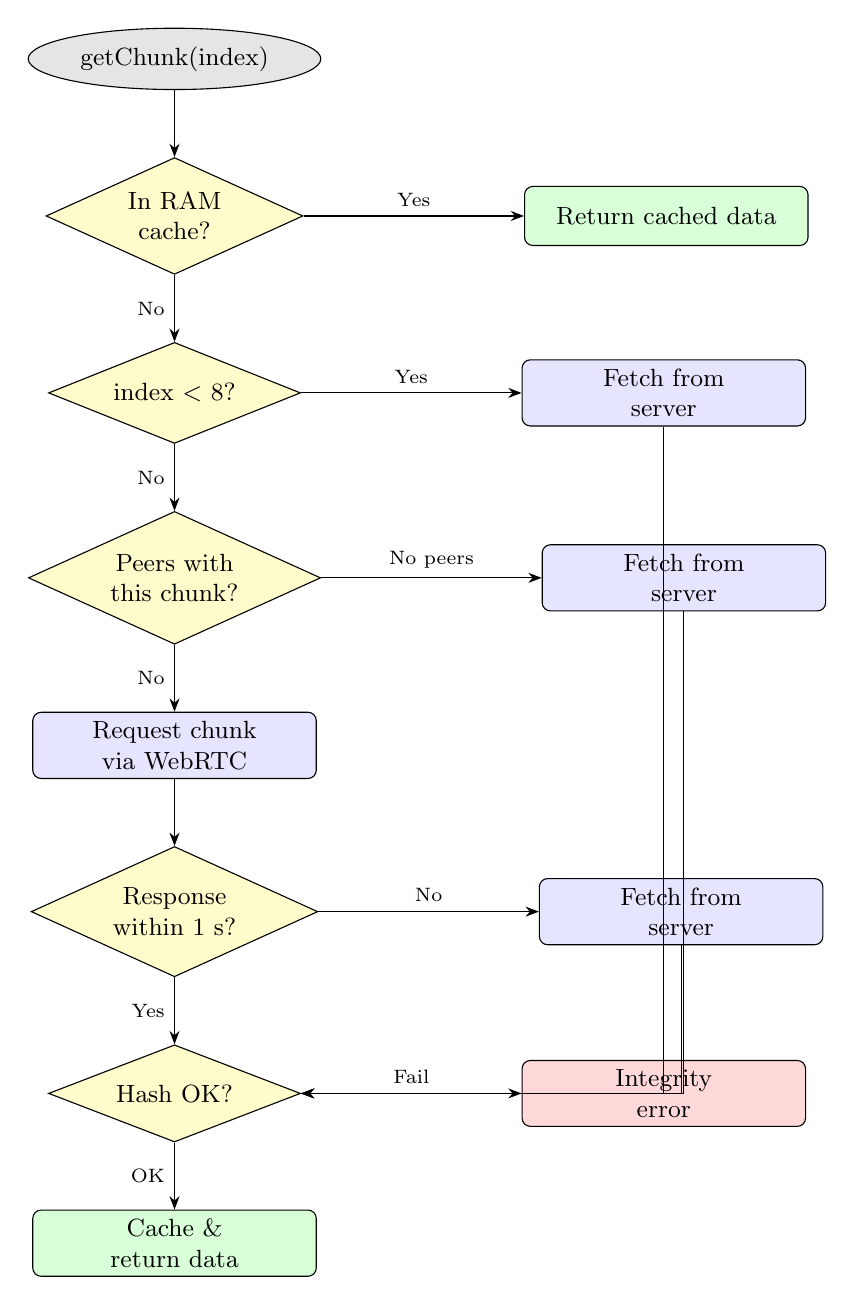
\begin{tikzpicture}[
  node distance=0.85cm and 0.1cm,
  startstop/.style={ellipse, draw, fill=gray!20,
                    minimum width=2.4cm, minimum height=0.7cm, font=\small},
  decision/.style={diamond, draw, fill=yellow!20, aspect=2.2,
                   minimum width=3.2cm, font=\small, align=center},
  process/.style={rectangle, draw, fill=blue!10, rounded corners=3pt,
                  minimum width=3.6cm, minimum height=0.75cm,
                  font=\small, align=center},
  good/.style={rectangle, draw, fill=green!15, rounded corners=3pt,
               minimum width=3.6cm, minimum height=0.75cm,
               font=\small, align=center},
  bad/.style={rectangle, draw, fill=red!15, rounded corners=3pt,
              minimum width=3.6cm, minimum height=0.75cm,
              font=\small, align=center},
  arr/.style={-{Stealth}}
]
  \node[startstop] (start) {getChunk(index)};

  \node[decision, below=of start] (inCache) {In RAM\\cache?};
  \node[good, right=2.8cm of inCache] (returnCache) {Return cached data};

  \node[decision, below=of inCache] (isPrefix) {index $<$ 8?};
  \node[process, right=2.8cm of isPrefix] (fetchServer1) {Fetch from\\server};

  \node[decision, below=of isPrefix] (hasPeers) {Peers with\\this chunk?};
  \node[process, right=2.8cm of hasPeers] (fetchServer2) {Fetch from\\server};

  \node[process, below=of hasPeers] (p2pReq)  {Request chunk\\via WebRTC};
  \node[decision, below=of p2pReq]  (timeout) {Response\\within 1 s?};
  \node[process, right=2.8cm of timeout] (fetchServer3) {Fetch from\\server};

  \node[decision, below=of timeout] (verify) {Hash OK?};
  \node[bad, right=2.8cm of verify] (integrity) {Integrity\\error};

  \node[good, below=of verify] (cache) {Cache \&\\return data};

  % edges
  \draw[arr] (start)      -- (inCache);
  \draw[arr] (inCache)    -- node[left, font=\scriptsize]{No}  (isPrefix);
  \draw[arr] (inCache)    -- node[above, font=\scriptsize]{Yes} (returnCache);
  \draw[arr] (isPrefix)   -- node[left, font=\scriptsize]{No}  (hasPeers);
  \draw[arr] (isPrefix)   -- node[above, font=\scriptsize]{Yes} (fetchServer1);
  \draw[arr] (fetchServer1.south) |- (verify.east);
  \draw[arr] (hasPeers)   -- node[left, font=\scriptsize]{No}  (p2pReq);
  \draw[arr] (hasPeers)   -- node[above, font=\scriptsize]{No peers} (fetchServer2);
  \draw[arr] (fetchServer2.south) |- (verify.east);
  \draw[arr] (p2pReq)     -- (timeout);
  \draw[arr] (timeout)    -- node[left, font=\scriptsize]{Yes} (verify);
  \draw[arr] (timeout)    -- node[above, font=\scriptsize]{No}  (fetchServer3);
  \draw[arr] (fetchServer3.south) |- (verify.east);
  \draw[arr] (verify)     -- node[left, font=\scriptsize]{OK}  (cache);
  \draw[arr] (verify)     -- node[above, font=\scriptsize]{Fail} (integrity);
\end{tikzpicture}
\caption{Chunk fetch decision flow inside \texttt{ChunkService.\_fetchChunkLogic}.}
\label{fig:chunk-fetch-flow}
\end{figure}

\subsection{Look-Ahead Prefetching}
\label{subsec:prefetch}

\par To prevent starvation of the audio decoder, the \texttt{ChunkService} maintains
a \texttt{\_preloadAhead} constant of 16.  After each call to \texttt{getChunk(i)},
the service asynchronously initiates fetches for chunks $i+1$ through $i+15$, subject
to the deduplication map preventing re-issuance.  These prefetch operations run
concurrently using \texttt{Future.wait}, so the one-second P2P timeout limits only
the latency of a single chunk, not the aggregate prefetch window.

% ─────────────────────────────────────────────────────────────────────────────
\section{P2P Audio Source and Range Request Handling}
\label{sec:audio-source}

\par The Flutter \texttt{just\_audio} library consumes audio through an abstract
\texttt{AudioSource} interface.  For P2P streaming the application provides
\texttt{P2PChunkedAudioSource}, which extends \texttt{StreamAudioSource} and
translates HTTP-style range requests into calls to \texttt{ChunkService.getChunk}.

\par When the audio player issues a range request for bytes $[s, e)$, the source:

\begin{enumerate}
  \item Clamps the range to $[0, \texttt{totalBytes})$.
  \item Computes the first and last chunk indices:
        $i_{\min} = \lfloor s / 65536 \rfloor$,
        $i_{\max} = \lfloor (e-1) / 65536 \rfloor$.
  \item Iterates from $i_{\min}$ to $i_{\max}$, awaiting each chunk future in turn
        while simultaneously scheduling a speculative fetch for chunk $i + 1$ to
        overlap network latency with audio decoding.
  \item For each chunk, computes the byte-level slice:
        $\texttt{sliceStart} = \max(0,\ s - i \cdot 65536)$,
        $\texttt{sliceEnd} = \min(|\texttt{chunk}|,\ e - i \cdot 65536)$,
        and yields the sub-list to the output stream.
\end{enumerate}

\par The response object declares \texttt{rangeRequestsSupported: true} and sets the
\texttt{Content-Length} header to $e - s$, allowing the audio player to issue
fine-grained seeks without re-downloading the entire file.

% ─────────────────────────────────────────────────────────────────────────────
\section{WebRTC Peer Management}
\label{sec:webrtc}

\par The \texttt{WebRTCService} on the client side manages the lifecycle of all
peer-to-peer connections.  It is constructed with references to the signaling
WebSocket and two callbacks: \texttt{onChunkReceived} (invoked when binary chunk
data arrives over a data channel) and \texttt{onChunkRequested} (invoked when a
peer requests a chunk that this device may be able to serve).

\subsection{Connection Establishment}
\label{subsec:conn-establish}

\par Peer connections are established using the standard WebRTC offer/answer
handshake.  When a \texttt{PEER\_BUFFER\_MAP} response arrives, the service
iterates the map and calls \texttt{\_createPeerConnection(peerId, initiator: true)}
for each newly discovered peer.  This method:

\begin{enumerate}
  \item Creates an \texttt{RTCPeerConnection} with the configured STUN servers
        (\texttt{stun.l.\allowbreak google.com:\allowbreak 19302} and
        \texttt{stun1.l.\allowbreak google.com:\allowbreak 19302}).
  \item Creates an ordered, reliable \texttt{RTCDataChannel} labelled
        \texttt{"chunk-channel"}.
  \item Generates an SDP offer, sets it as the local description, and transmits
        it to the signaling server as an \texttt{OFFER} message.
\end{enumerate}

\par The remote peer receives the offer, creates a mirrored connection with
\texttt{initiator: false}, sets the remote description, and replies with an
\texttt{ANSWER} message.  Both sides then exchange \texttt{ICE\_CANDIDATE} messages
until connectivity is established.  ICE candidates that arrive before the remote
description is set are queued in \texttt{\_iceQueues} and applied once the
description is available.

\subsection{Chunk Exchange Protocol}
\label{subsec:chunk-protocol}

\par Once the data channel is open, chunk requests and responses follow a simple
binary protocol.  A \emph{request} is sent as a UTF-8 text message with the format:

\begin{center}
  \texttt{REQUEST\_CHUNK:\{songId\}:\{chunkIndex\}}
\end{center}

\par A \emph{response} is a binary message whose first eight bytes form a header:
bytes 0–3 contain the \texttt{songId} as a big-endian 32-bit unsigned integer,
bytes 4–7 contain the \texttt{chunkIndex} in the same encoding, and the remaining
bytes are the raw audio data.  The receiving side strips the header and delivers the
payload bytes to the appropriate \texttt{ChunkService} via the
\texttt{resolvePeerRequest(chunkIndex, data)} callback.

\par If a chunk request arrives while the data channel is still in the
\texttt{connecting} state, the request is enqueued in
\texttt{\_pending\-ChunkRequests} and flushed via
\texttt{\_drain\-Pending\-Requests} as soon as the channel transitions to
\texttt{open}.  This prevents race conditions during the brief window between
peer discovery and channel readiness.

% ─────────────────────────────────────────────────────────────────────────────
\section{Audio Service and Playback State Management}
\label{sec:audio-service}

\par \texttt{AppAudioService} is the top-level coordinator for audio playback on the
client.  It owns the \texttt{just\_audio} \texttt{AudioPlayer} (or the
\texttt{media\_kit} equivalent on Linux and Windows), manages the song queue, and
bridges playback events to the data synchronisation and peer registry subsystems.

\subsection{Queue and Audio Source Selection}
\label{subsec:queue}

\par When the user starts a song, \texttt{setQueueAndPlay} atomically replaces the
queue and calls \texttt{\_buildAudioSource(song)}.  The factory branches on three
cases: if the song has a local file path, a \texttt{Uri.file} source is returned;
if the platform is web, a server-side stream URL is used; otherwise a \texttt{P2PChunkedAudioSource} is constructed, which triggers a
\texttt{ChunkService} instantiation and a manifest fetch.

\subsection{Proactive Prefix Caching}
\label{subsec:proactive-cache}

\par To reduce the latency of switching to the next song in the queue, the service
runs \texttt{\_proactivelyCachePrefixes} each time a new song begins.  This method
inspects the next five songs in the queue and, for each one, issues a server
prefix fetch for the first eight chunks.  Because the prefix is a single HTTP call
returning 500~KiB, it can be stored in the disk cache well before the user reaches
that position in the queue, making the subsequent peer-negotiation phase overlap
with warm cache hits rather than cold fetches.

\subsection{Stuck-Playback Detection}
\label{subsec:stuck}

\par Network jitter or slow peer responses can occasionally stall the audio decoder
without triggering a formal error state.  \texttt{AppAudioService} runs a watchdog
timer that samples the playback position every 500 milliseconds.  If the position
has not advanced after two consecutive samples (i.e., a 1000-millisecond window)
while the player is nominally in the \texttt{playing} state, the service pauses,
seeks to the current position, and resumes.  This sequence forces the player to
re-issue range requests, which in turn triggers fresh chunk fetches that may select
a different peer or fall through to the server, resolving the stall.

\subsection{Persistent Playback State}
\label{subsec:playback-state}

\par Every 30 seconds while playback is active, \texttt{push\-State\-To\-Server}
serialises the current queue as a JSON array of song IDs, the playback position in
milliseconds, and the shuffle and repeat flags into a \texttt{PlaybackStateDto},
which is sent to the \texttt{PlaybackRestService} REST endpoint.  On application
startup, \texttt{restore\-From\-Server\-State} fetches the last saved state and
reconstructs the queue and position, enabling seamless handoff between devices and
resumption after application restarts.

% ─────────────────────────────────────────────────────────────────────────────
\section{End-to-End Flows}
\label{sec:flows}

\par This section consolidates the subsystem descriptions above into three end-to-end flow diagrams that emphasise the temporal ordering of operations and the interactions between components.

\subsection{Playback Initialisation Flow}
\label{subsec:flow-init}

\par Figure~\ref{fig:flow-init} shows the sequence of operations from the moment a
user selects a song to the moment audio begins playing.  The critical property is that playback starts after the server prefix completes (typically within one round-trip time) while peer connection establishment continues asynchronously in the background.

\begin{figure}[htbp]
\centering
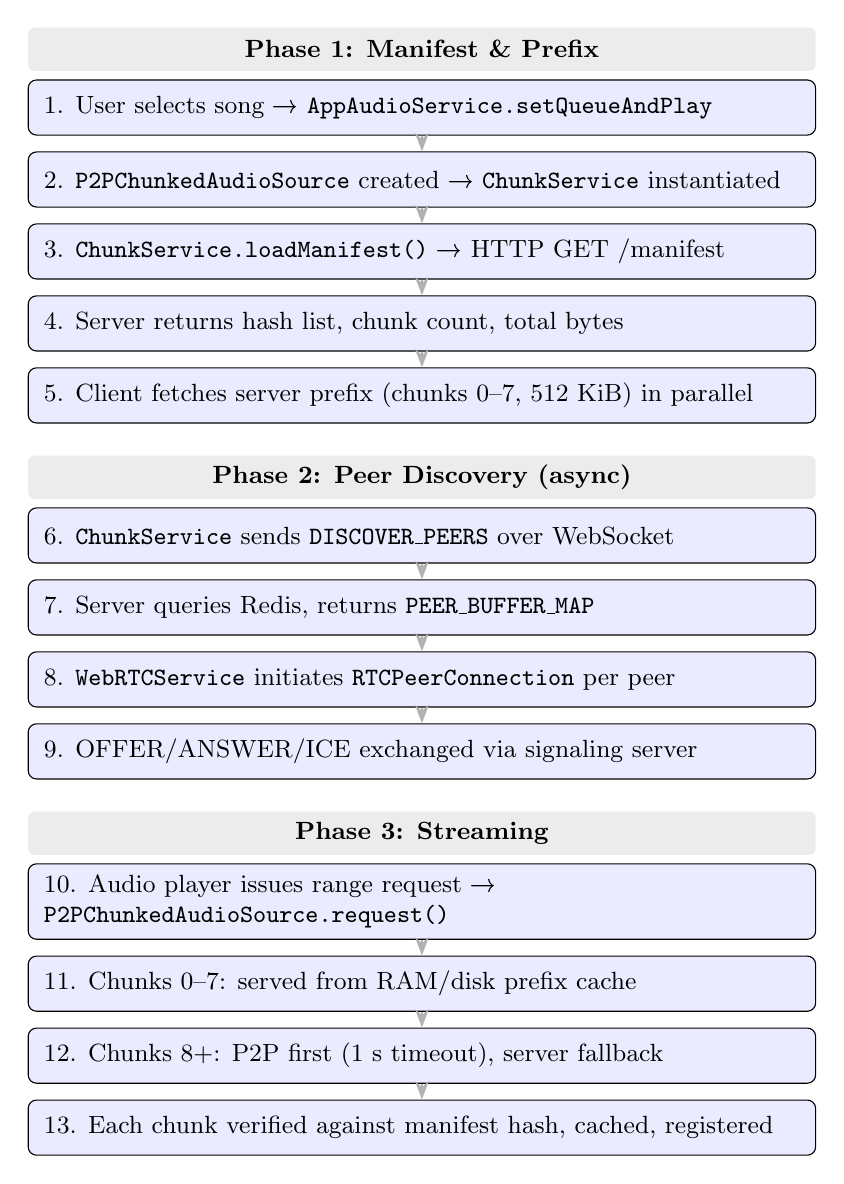
\begin{tikzpicture}[
  node distance=0.7cm,
  box/.style={rectangle, draw, fill=blue!8, rounded corners=3pt,
              minimum width=10cm, minimum height=0.7cm,
              font=\small, align=flush left, text width=9.6cm,
              inner sep=4pt},
  phase/.style={rectangle, draw=none, fill=gray!15, rounded corners=2pt,
                minimum width=10cm, minimum height=0.55cm,
                font=\small\bfseries, align=center},
  arr/.style={-{Stealth}, thick, gray!60}
]
  \node[phase]                  (p1) {Phase 1: Manifest \& Prefix};
  \node[box, below=0.1cm of p1] (s1) {1. User selects song → \texttt{AppAudioService.setQueueAndPlay}};
  \node[box, below=0.2cm of s1] (s2) {2. \texttt{P2PChunkedAudioSource} created → \texttt{ChunkService} instantiated};
  \node[box, below=0.2cm of s2] (s3) {3. \texttt{ChunkService.loadManifest()} → HTTP GET /manifest};
  \node[box, below=0.2cm of s3] (s4) {4. Server returns hash list, chunk count, total bytes};
  \node[box, below=0.2cm of s4] (s5) {5. Client fetches server prefix (chunks 0–7, 512 KiB) in parallel};

  \node[phase, below=0.4cm of s5] (p2) {Phase 2: Peer Discovery (async)};
  \node[box, below=0.1cm of p2]  (s6) {6. \texttt{ChunkService} sends \texttt{DISCOVER\_PEERS} over WebSocket};
  \node[box, below=0.2cm of s6]  (s7) {7. Server queries Redis, returns \texttt{PEER\_BUFFER\_MAP}};
  \node[box, below=0.2cm of s7]  (s8) {8. \texttt{WebRTCService} initiates \texttt{RTCPeerConnection} per peer};
  \node[box, below=0.2cm of s8]  (s9) {9. OFFER/ANSWER/ICE exchanged via signaling server};

  \node[phase, below=0.4cm of s9]  (p3) {Phase 3: Streaming};
  \node[box, below=0.1cm of p3]   (s10) {10. Audio player issues range request → \texttt{P2PChunkedAudioSource.request()}};
  \node[box, below=0.2cm of s10]  (s11) {11. Chunks 0–7: served from RAM/disk prefix cache};
  \node[box, below=0.2cm of s11]  (s12) {12. Chunks 8+: P2P first (1 s timeout), server fallback};
  \node[box, below=0.2cm of s12]  (s13) {13. Each chunk verified against manifest hash, cached, registered};

  \draw[arr] (s1.south) -- (s2.north);
  \draw[arr] (s2.south) -- (s3.north);
  \draw[arr] (s3.south) -- (s4.north);
  \draw[arr] (s4.south) -- (s5.north);
  \draw[arr] (s6.south) -- (s7.north);
  \draw[arr] (s7.south) -- (s8.north);
  \draw[arr] (s8.south) -- (s9.north);
  \draw[arr] (s10.south) -- (s11.north);
  \draw[arr] (s11.south) -- (s12.north);
  \draw[arr] (s12.south) -- (s13.north);
\end{tikzpicture}
\caption{Playback initialisation flow from song selection to streaming.}
\label{fig:flow-init}
\end{figure}

\subsection{Chunk Delivery Decision Flow}
\label{subsec:flow-chunk}

\par The chunk delivery path (Figure~\ref{fig:chunk-fetch-flow}, reproduced schematically here for emphasis) is the innermost hot path of the system.  Its design reflects two competing constraints: \emph{latency} (the audio decoder cannot buffer ahead if chunk fetches are slow) and \emph{server cost} (the goal is to minimise origin-server bandwidth).
The prefix threshold of eight chunks resolves this tension by guaranteeing a baseline supply of data from a reliable source while exploiting the observation that WebRTC connections take on the order of hundreds of milliseconds to negotiate, longer than it takes to drain the eight-chunk prefix at typical decoding rates.

\par The one-second P2P timeout was chosen empirically to balance the risk of peer
starvation against the benefit of peer offloading.  If a peer is temporarily unavailable, the one-second wait is short enough that the audio player's internal buffer (fed by the 16-chunk lookahead) absorbs the latency without an audible glitch.

\subsection{Library Synchronisation Flow}
\label{subsec:flow-sync}

\par Figure~\ref{fig:flow-sync} shows the multi-device library sync triggered by a user action such as liking a song or deleting a track from the library.

\begin{figure}[htbp]
\centering
\resizebox{\textwidth}{!}{%
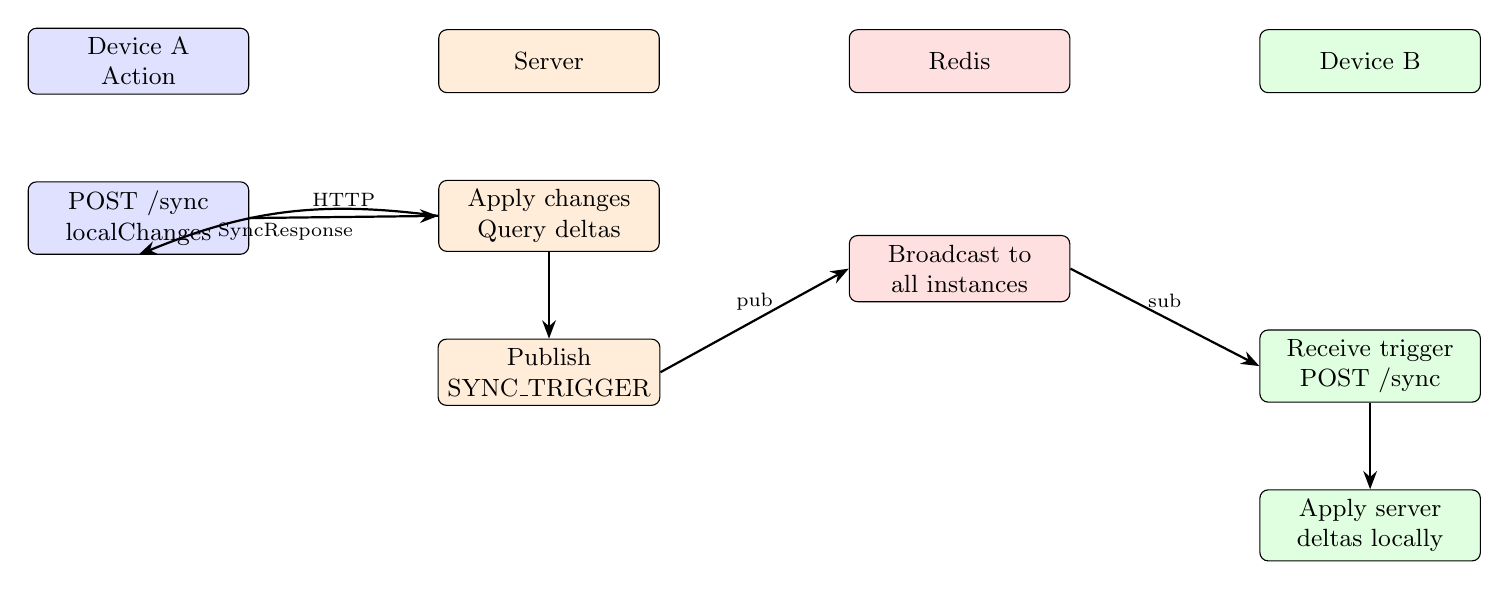
\begin{tikzpicture}[
  node distance=1.1cm and 3.0cm,
  box/.style={rectangle, draw, rounded corners=3pt,
              minimum width=2.8cm, minimum height=0.8cm,
              font=\small, align=center},
  devA/.style={box, fill=blue!12},
  server/.style={box, fill=orange!15},
  redis/.style={box, fill=red!12},
  devB/.style={box, fill=green!12},
  arr/.style={-{Stealth}, thick}
]
  % Column headers
  \node[devA]    (a1) {Device A\\Action};
  \node[server, right=2.4cm of a1]  (srv) {Server};
  \node[redis, right=2.4cm of srv]  (red) {Redis};
  \node[devB, right=2.4cm of red]   (b1)  {Device B};

  % Steps
  \node[devA, below=of a1]   (a2) {POST /sync\\localChanges};
  \node[server, below=of srv] (sv2) {Apply changes\\Query deltas};
  \node[server, below=of sv2] (sv3) {Publish\\SYNC\_TRIGGER};
  \node[redis, below=1.8cm of red]  (r1)  {Broadcast to\\all instances};
  \node[devB, below=3.0cm of b1]   (b2)  {Receive trigger\\POST /sync};
  \node[devB, below=of b2]   (b3)  {Apply server\\deltas locally};

  % Arrows
  \draw[arr] (a2.east)  -- node[above,font=\scriptsize]{HTTP}   (sv2.west);
  \draw[arr] (sv2.south)-- (sv3.north);
  \draw[arr] (sv3.east) -- node[above,font=\scriptsize]{pub}    (r1.west);
  \draw[arr] (r1.east)  -- node[above,font=\scriptsize]{sub}    (b2.west);
  \draw[arr] (b2.south) -- (b3.north);
  % Response arrow
  \draw[arr] (sv2.west) to[bend right=15]
              node[below,font=\scriptsize]{SyncResponse} (a2.south);
\end{tikzpicture}%
}
\caption{Multi-device library synchronisation triggered by a user action on Device A.}
\label{fig:flow-sync}
\end{figure}

% ─────────────────────────────────────────────────────────────────────────────
\section{Delivery Statistics and Observability}
\label{sec:stats}

\par To validate the effectiveness of the peer-assisted approach, the system records
per-session delivery statistics in the \texttt{ChunkStat} entity.  Each row captures
\texttt{p2pChunks}, \texttt{serverChunks}, \texttt{totalChunks}, and a derived
\texttt{p2p\-Percentage}.  The \texttt{ChunkService} accumulates counts as each chunk is fetched and fires the \texttt{\_onFully\-Received} callback when the last chunk of a song has been delivered, passing a \texttt{ChunkDelivery\-Stats} value object that the \texttt{AppAudioService} forwards to the REST statistics endpoint.

\par These records allow an operator to observe, for a given deployment, what fraction of total data volume is served by peers rather than the origin server.  Under favourable conditions (an audience that contains several listeners of the same song) the peer offload ratio should approach the theoretical maximum of
$(N - 1) / N$ for a swarm of $N$ simultaneous listeners sharing the same track,
limited in practice by the prefix requirement and connection churn.

\chapter{Graphical Interface and Application Execution}
\label{chap:ch4}

\tolerance=9999
\emergencystretch=3em

\indent \par Chapter \ref{chap:ch3} described how the system was built. This chapter describes how it actually looks and behaves once it is running. The discussion is split in three parts. The first part presents the graphical interface as a whole, screen by screen, so the reader can map the abstract components from the previous chapter to the actual buttons and panels he would see on his own machine. The second part is a mini walkthrough of the main functionality, peer-assisted streaming, as a user would experience it from the home screen up to the statistics view. The third part consolidates the steps into a short user manual.

\par Throughout the chapter, the screenshots are taken from the macOS build of the application, with a small library imported from disk and a single user signed in. The authentication flow itself is documented in Section \ref{subsec:auth} of the previous chapter and does not have its own screenshot here. All the screens have a persistent navigation drawer on the left and a persistent player bar at the bottom; the middle area is what changes when the user moves between sections.


\section{The Graphical Interface}
\label{sec:gui}

\subsection{Home and Main Scaffold}
\label{subsec:gui-home}

\indent \par Figure \ref{fig:screen-home} shows the home screen, which is the first screen the user sees after the bootstrap completes. The left drawer lists the seven destinations of the application: Home, Albums, Artists, Music (the tracks list), Playlists, Upload songs and Statistics. The user settings entry is at the bottom of the drawer, and shows the email of the currently signed-in user.

\par The middle area of the home screen is composed of three horizontal rails: ``Jump back in'' with the recently played albums, ``Recommended for you'' with suggestions based on the listening history, and ``Rediscover'' with songs that the user has not listened to in a while. Each card displays the cover art, the title and the artist name. The persistent player bar at the bottom shows the currently playing song, the lyrics line at the centre, and the playback controls on the right (shuffle, previous, play/pause, next, repeat, and expand).

\begin{figure}[htbp]
\centering
\includegraphics[width=\textwidth]{figures/screenshots/home_screen.png}
\caption{Home screen with the navigation drawer, the three home rails (jump back in, recommended, rediscover), and the persistent player bar.}
\label{fig:screen-home}
\end{figure}

\subsection{Browsing the Catalogue}
\label{subsec:gui-catalogue}

\indent \par The catalogue can be browsed in three different ways, depending on what the user is looking for. The Music entry in the drawer opens the tracks view, shown in Figure \ref{fig:screen-tracks}. Songs are laid out as a grid of cover art with the title underneath; a search bar at the top filters by track name and the icons in the top right control sorting and shuffling.

\begin{figure}[htbp]
\centering
\includegraphics[width=\textwidth]{figures/screenshots/tracks_screen.png}
\caption{Tracks view, opened from the Music entry in the drawer. The grid is filterable through the search bar and sortable through the controls in the top right.}
\label{fig:screen-tracks}
\end{figure}

\par The Albums and Artists entries open similar grid views, focused on albums and on artists respectively. Figure \ref{fig:screen-albums} shows the albums view and Figure \ref{fig:screen-artists} the artists view. Selecting an album opens its detail page with the track listing; selecting an artist opens its detail page with both the artist's albums and his songs.

\begin{figure}[htbp]
\centering
\includegraphics[width=\textwidth]{figures/screenshots/albums_screen.png}
\caption{Albums view.}
\label{fig:screen-albums}
\end{figure}

\begin{figure}[htbp]
\centering
\includegraphics[width=\textwidth]{figures/screenshots/artists_screen.png}
\caption{Artists view.}
\label{fig:screen-artists}
\end{figure}

\subsection{Playlists}
\label{subsec:gui-playlists}

\indent \par The Playlists entry in the drawer opens the playlists view, depicted in Figure \ref{fig:screen-playlists}. The user can create new playlists, rename them, and reorder the songs inside. The built-in ``Liked Songs'' playlist is always present, marked indestructible at the database level (see Section \ref{subsec:schema-user}) so that it cannot be deleted by accident.

\begin{figure}[htbp]
\centering
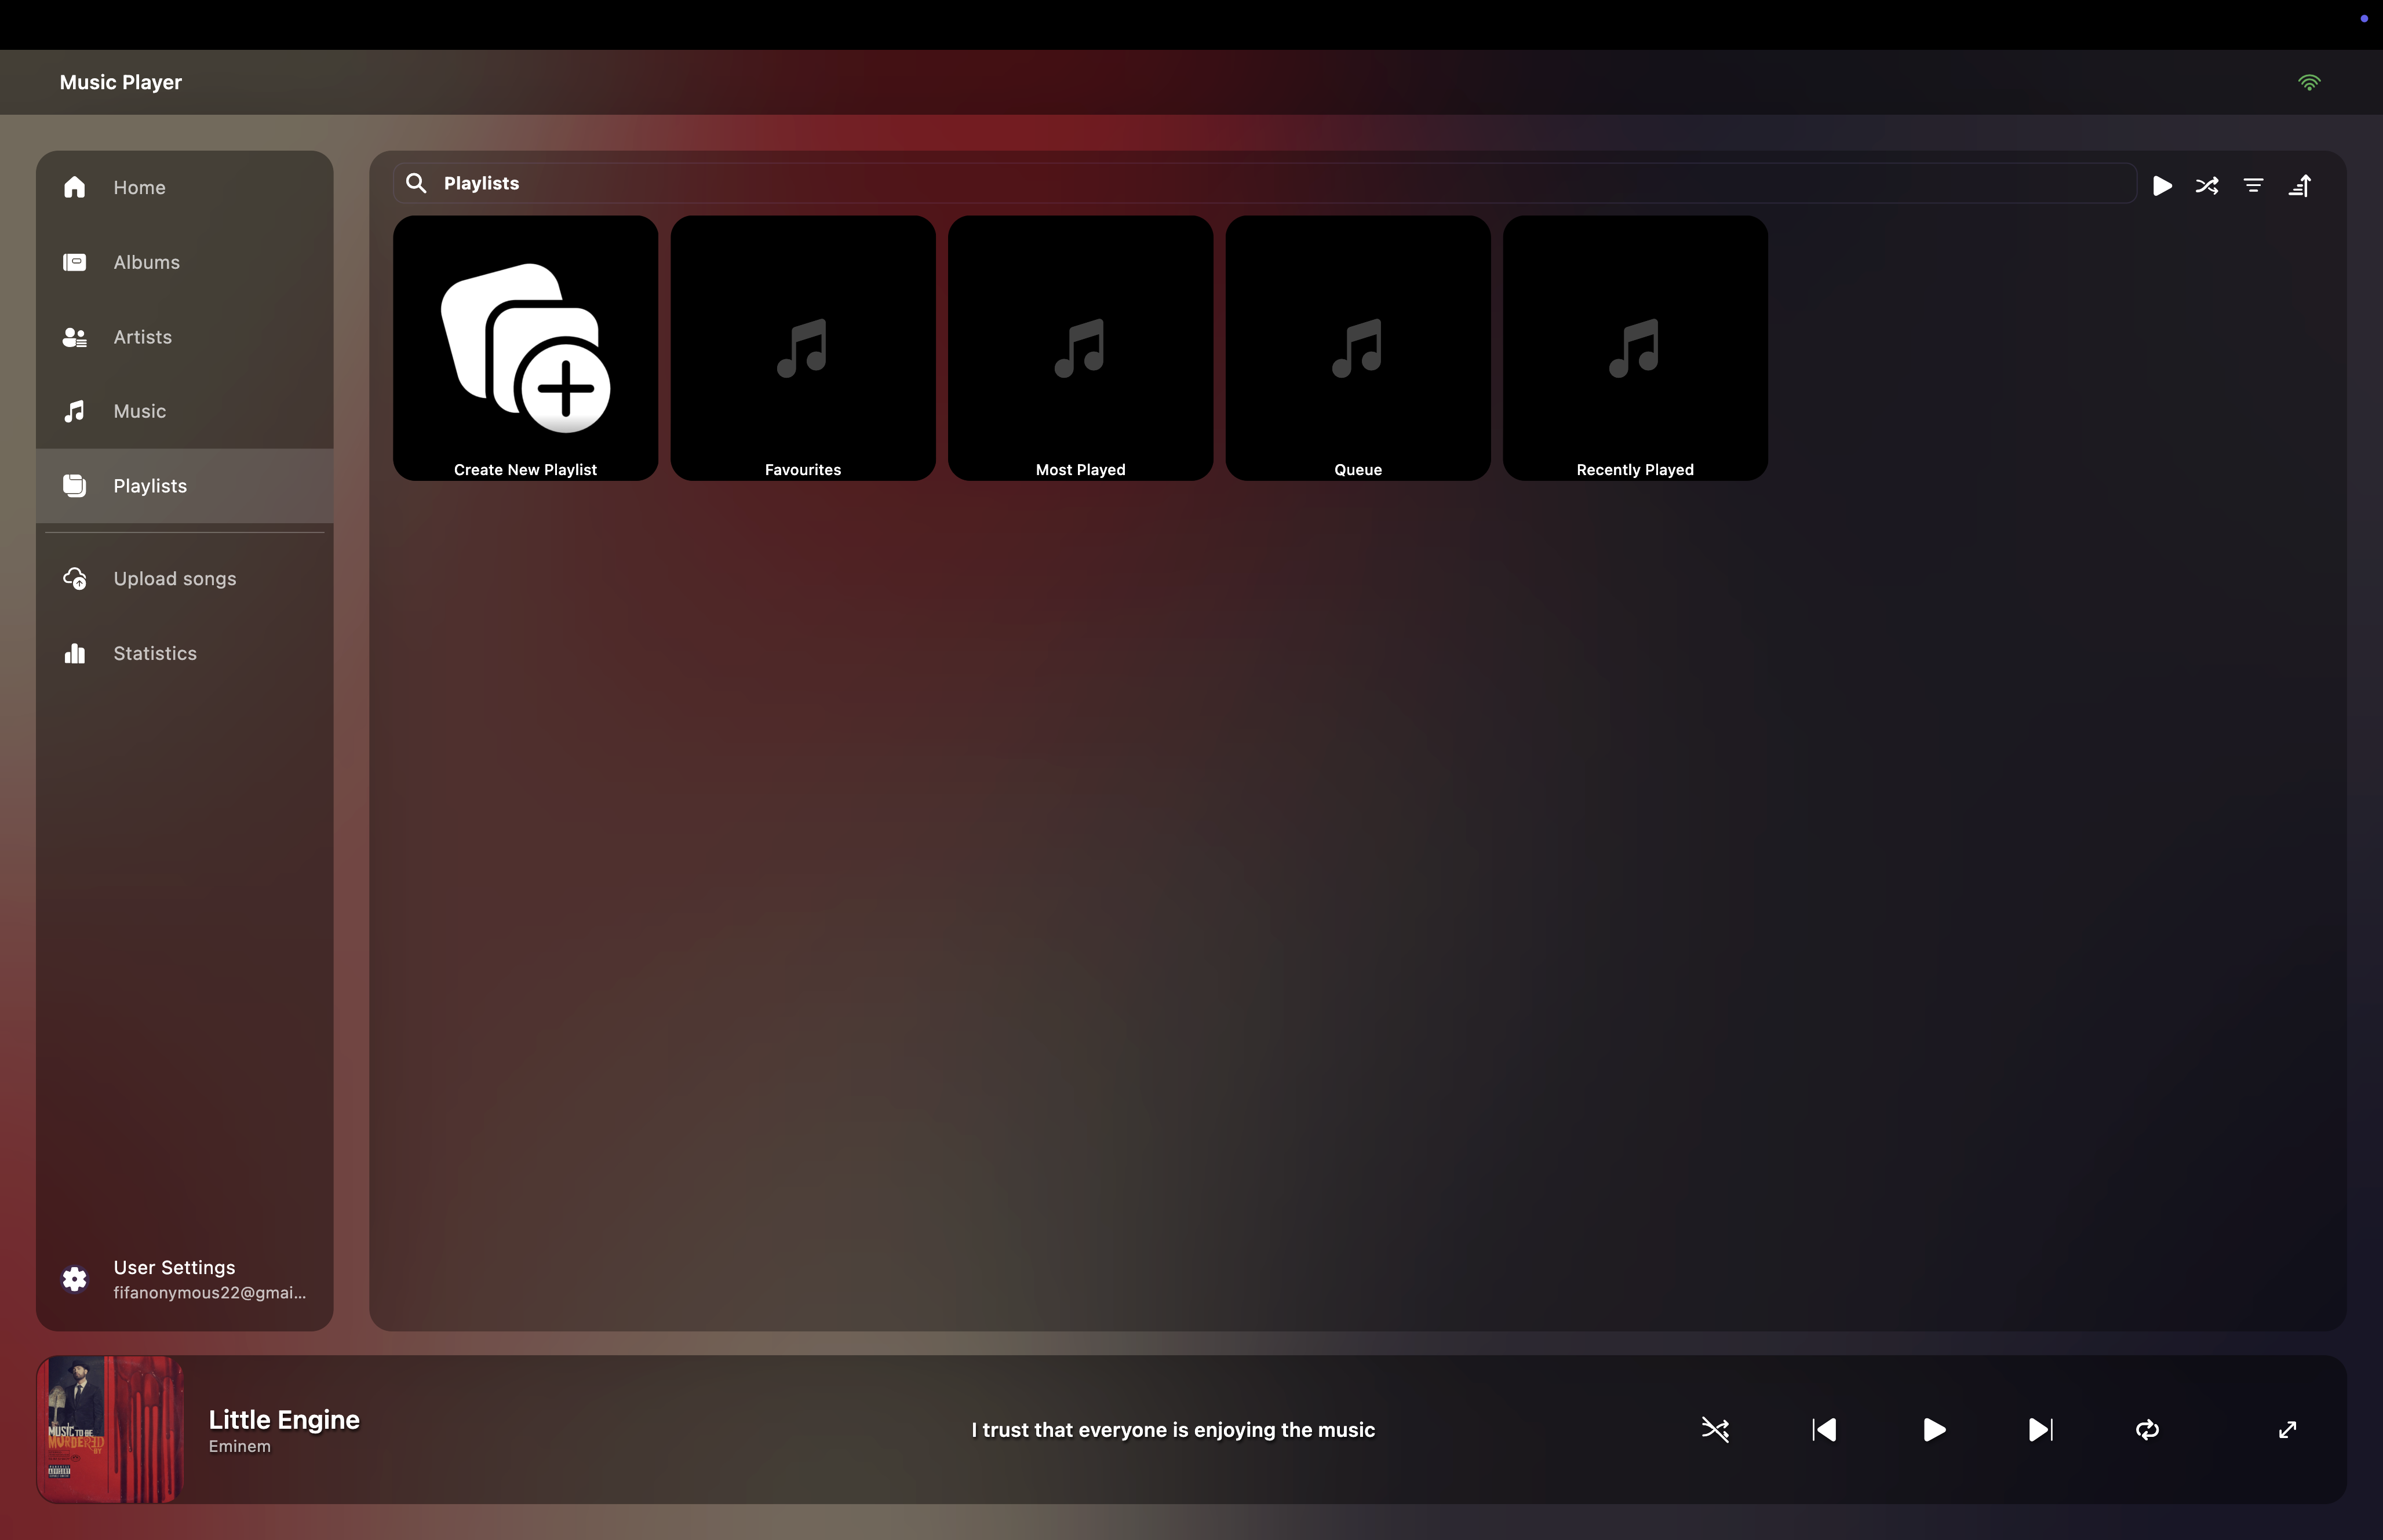
\includegraphics[width=\textwidth]{figures/screenshots/playlists_screen.png}
\caption{Playlists view.}
\label{fig:screen-playlists}
\end{figure}

\subsection{Now Playing}
\label{subsec:gui-now-playing}

\indent \par Tapping on the player bar at the bottom of the scaffold expands it into the now playing screen, shown in Figure \ref{fig:screen-now-playing}. The middle section displays the cover art of the currently playing song; the left side shows the lyrics, when available, scrolled along the playback position; the right side shows the upcoming queue. A heart icon on the cover toggles the liked state, which fires a \texttt{PATCH /songs/\{fileHash\}} request as described in Section \ref{subsec:state-sync}. The progress bar and the standard playback controls run along the bottom.

\begin{figure}[htbp]
\centering
\includegraphics[width=\textwidth]{figures/screenshots/expanded_music_player_widget.png}
\caption{Expanded now playing screen with the lyrics on the left, the cover in the centre, and the queue on the right.}
\label{fig:screen-now-playing}
\end{figure}

\subsection{Uploading Songs}
\label{subsec:gui-upload}

\indent \par The Upload songs entry in the drawer opens the upload screen, shown empty in Figure \ref{fig:screen-upload-empty}. The user selects one or more audio files from disk; each file is added to the upload list and shown with its title and artist as parsed from the file's metadata, as in Figure \ref{fig:screen-upload-song}. Pressing the Upload button runs the negotiated upload protocol from Section \ref{subsec:upload}: the client first calls \texttt{POST /songs/negotiate} with the manifest of chunk hashes, and then sends only the missing chunks through \texttt{POST /songs/\{fileHash\}/chunks/\{chunkIndex\}}.

\begin{figure}[htbp]
\centering
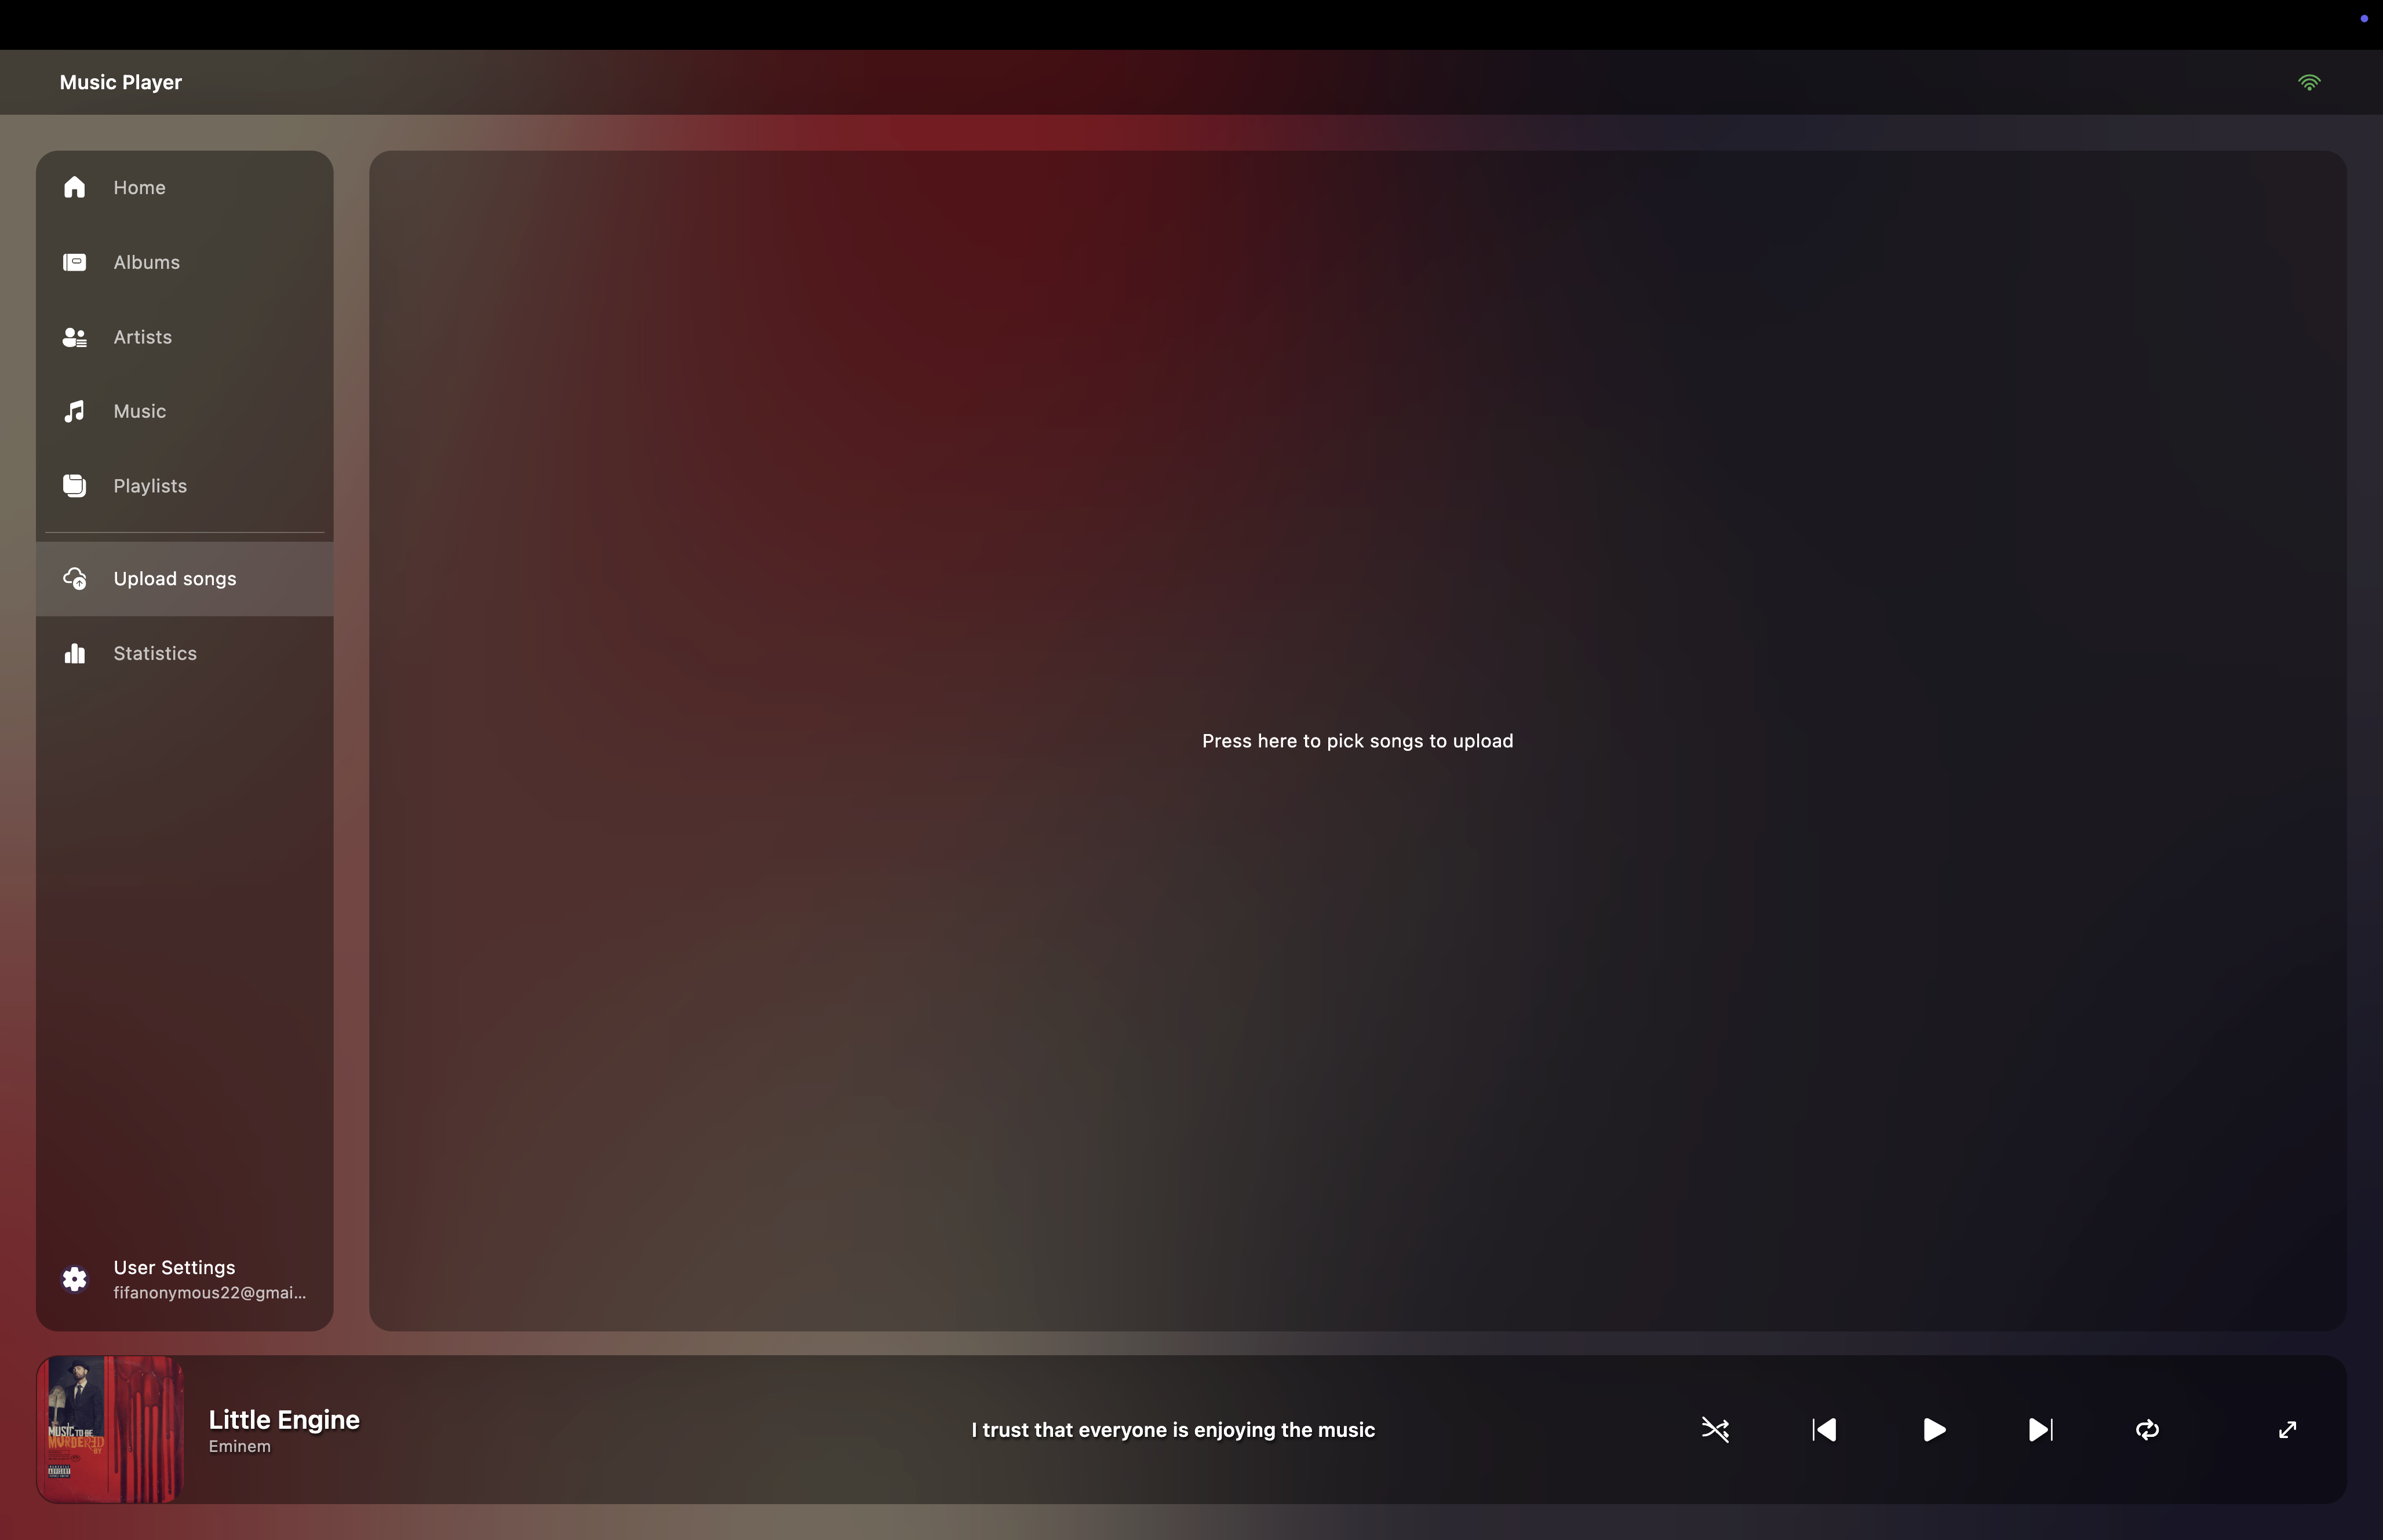
\includegraphics[width=\textwidth]{figures/screenshots/upload_screen_empty.png}
\caption{Upload screen, empty. The placeholder invites the user to pick songs from disk.}
\label{fig:screen-upload-empty}
\end{figure}

\begin{figure}[htbp]
\centering
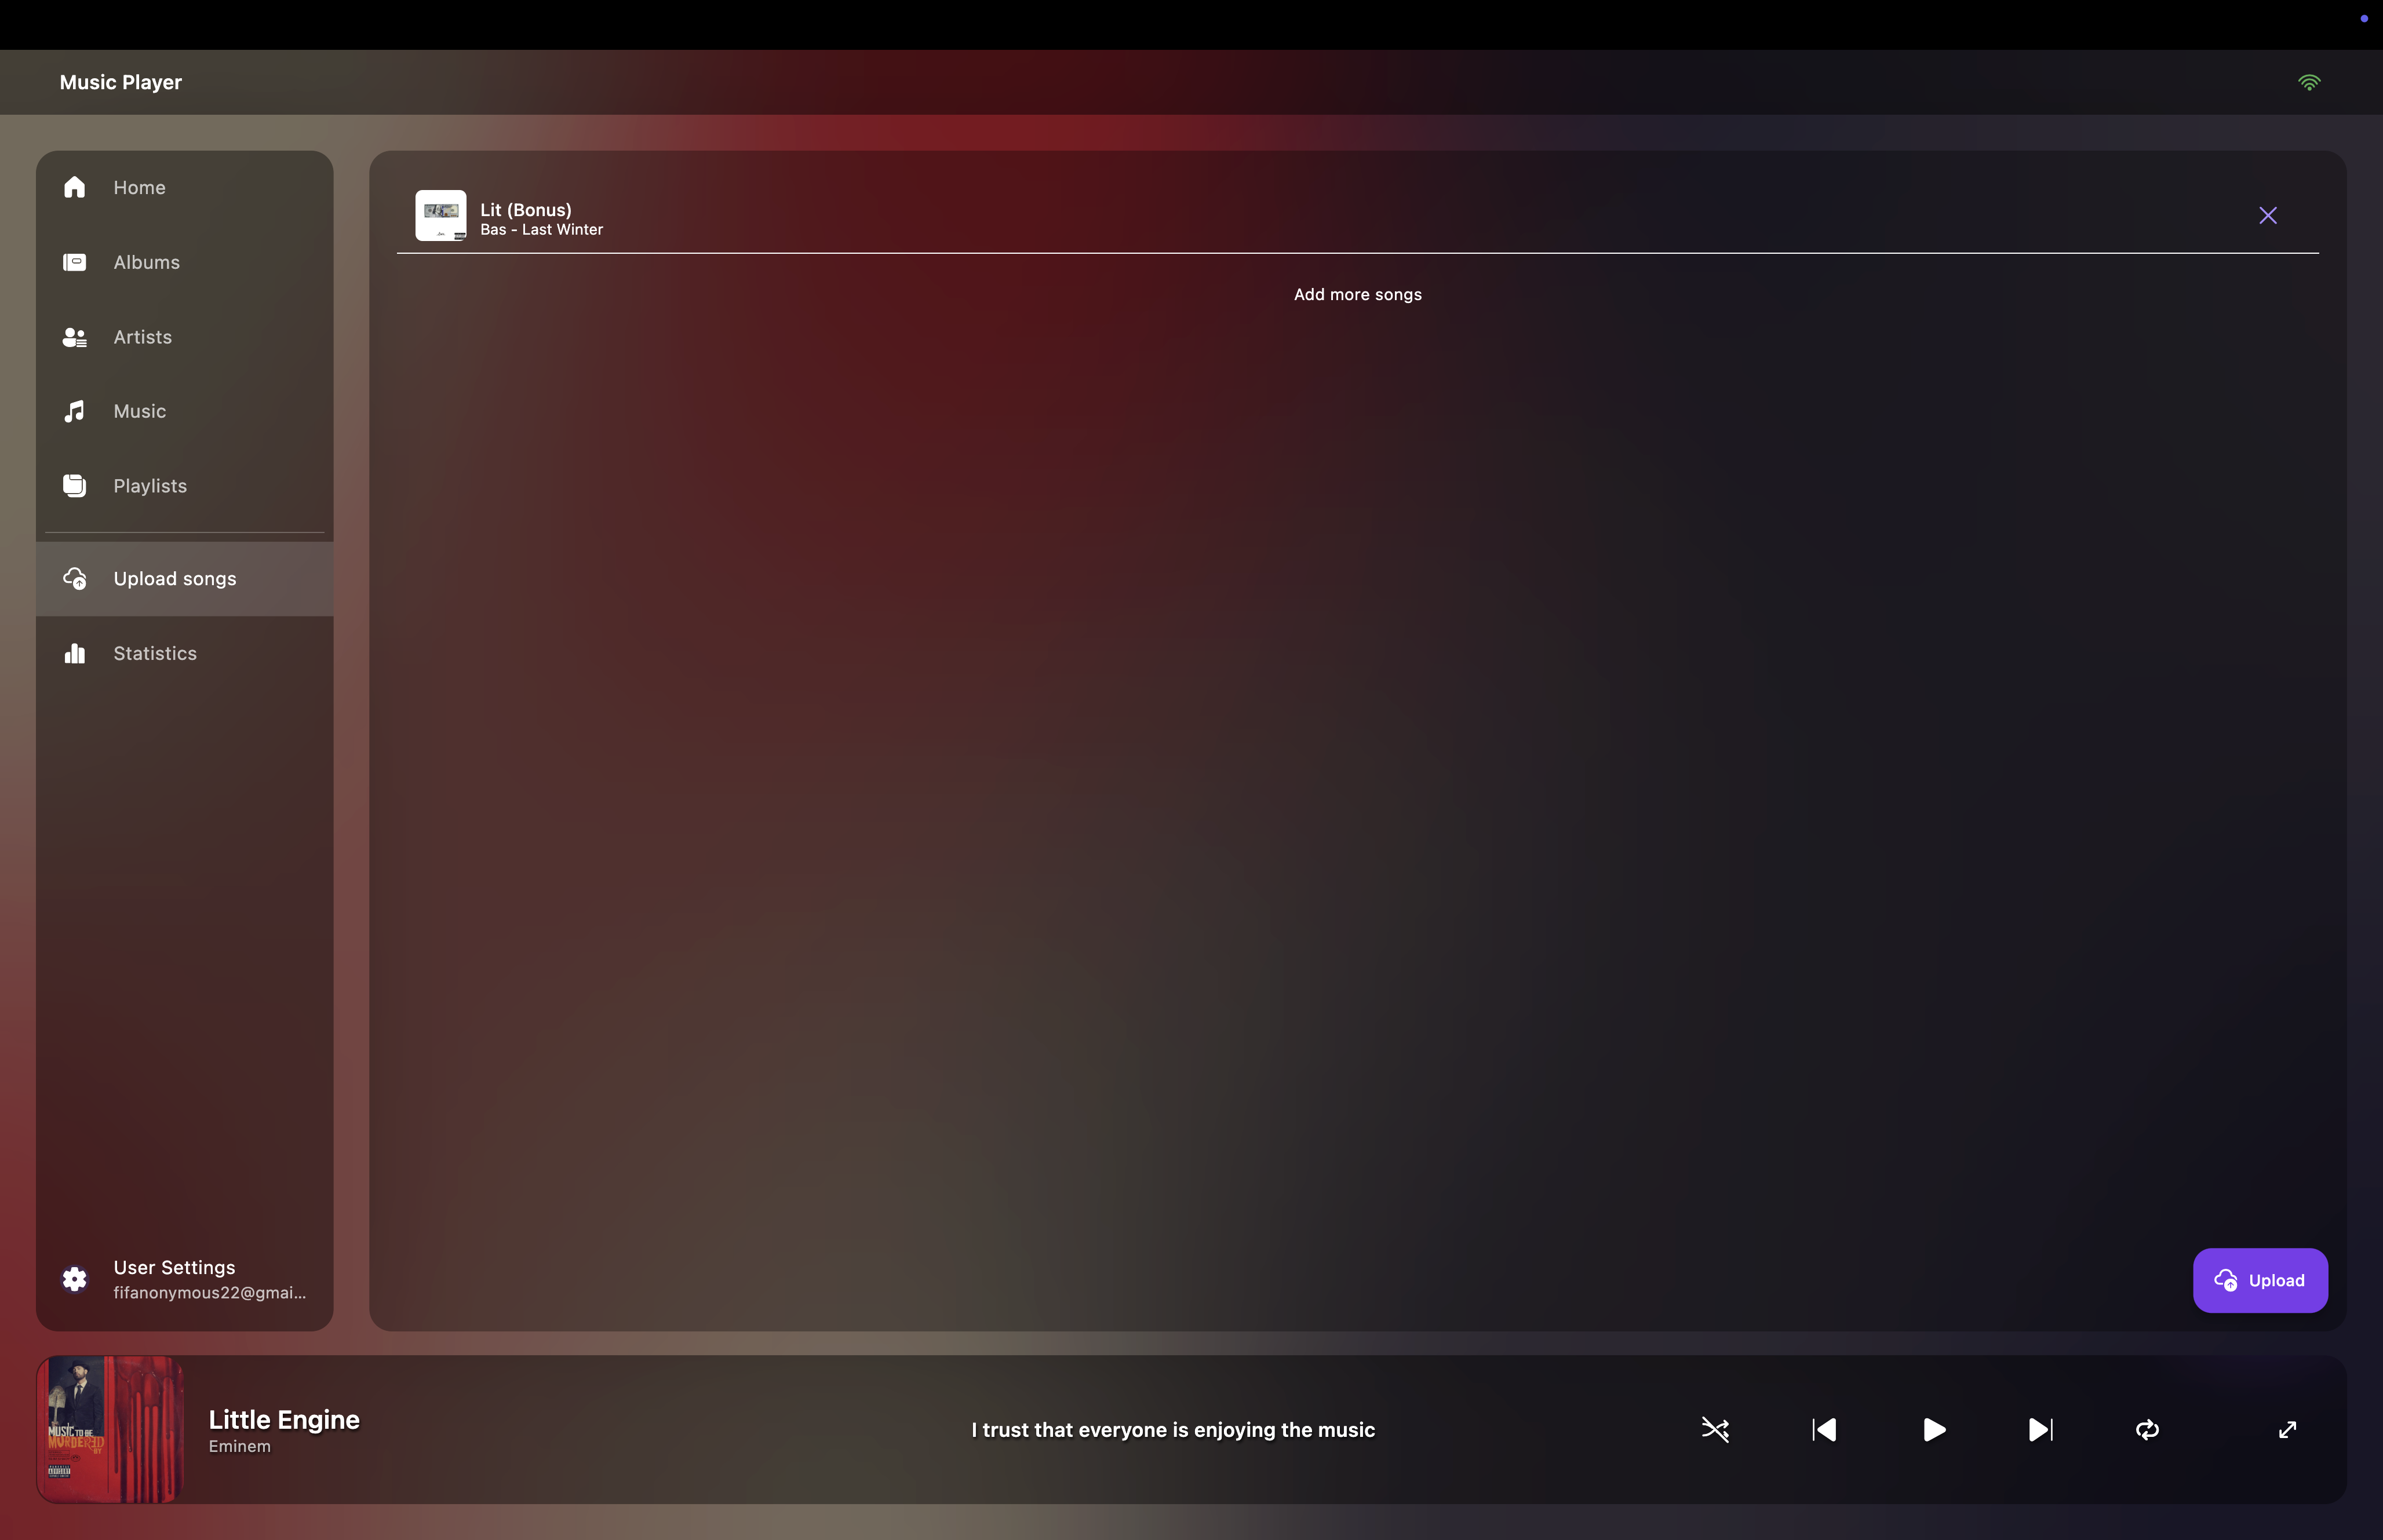
\includegraphics[width=\textwidth]{figures/screenshots/upload_screen_song.png}
\caption{Upload screen with one song queued, ready to be sent through the negotiated upload protocol.}
\label{fig:screen-upload-song}
\end{figure}

\subsection{Settings}
\label{subsec:gui-settings}

\indent \par The User Settings entry at the bottom of the drawer opens the settings screen, shown in Figure \ref{fig:screen-settings}. The exposed options are kept intentionally short. The Account row shows the signed-in user and a Logout button. The Playback Speed slider sets the global playback rate. The Peer Network dropdown selects the connection types on which the application is allowed to act as a peer (Wi-Fi only, Cellular only, or both), as described in Section \ref{subsec:upload-limits}. The WiFi Data Limit and Cellular Data Limit sliders set the monthly upload caps for each type of connection.

\begin{figure}[htbp]
\centering
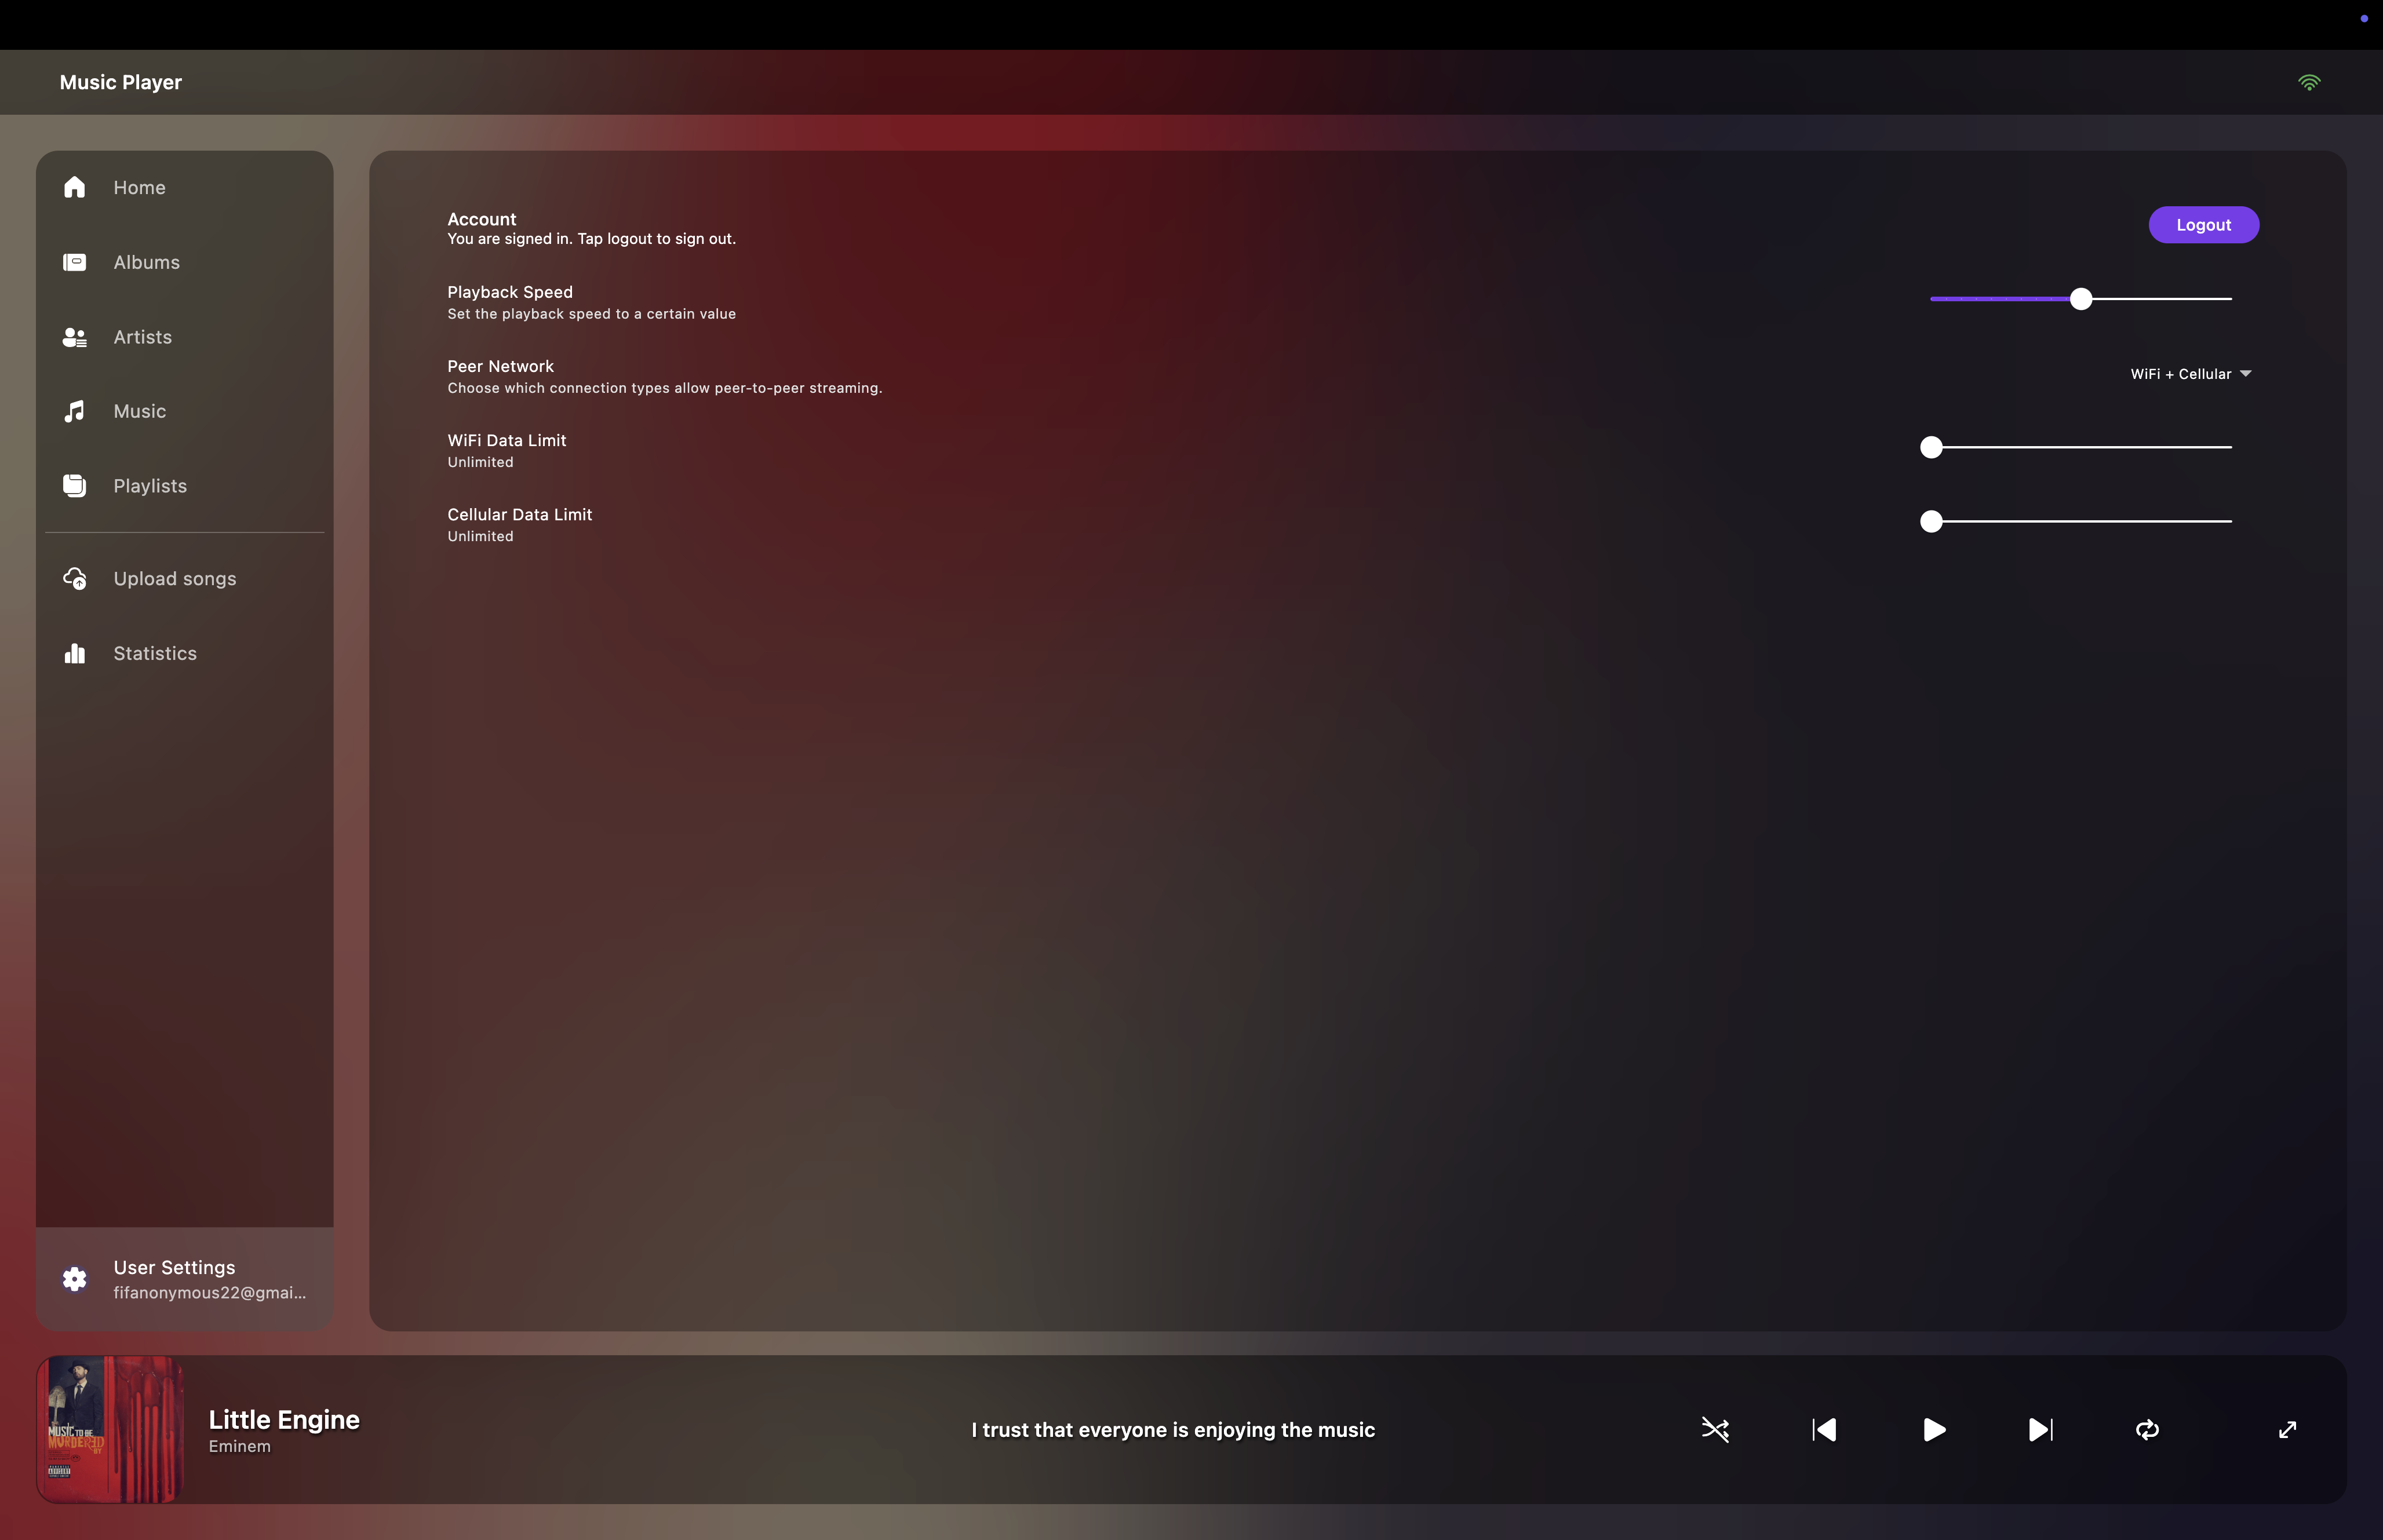
\includegraphics[width=\textwidth]{figures/screenshots/settings_screen.png}
\caption{Settings screen, with the account, the playback speed, and the peer network options.}
\label{fig:screen-settings}
\end{figure}

\subsection{Statistics}
\label{subsec:gui-stats}

\indent \par The Statistics entry in the drawer opens the screen shown in Figure \ref{fig:screen-stats}, which is the user-visible representation of the \texttt{chunk\_stats} rows described in Section \ref{subsec:schema-aux}. The card at the top aggregates the entire history: the average P2P share, the cumulative number of P2P chunks, the cached chunks, the local files, and the total chunks ever served. Below the card, every recorded session is shown as its own row, with the song name, the per-session P2P percentage on the right, the source breakdown (server/peer/local) underneath the title, and the timestamp on the bottom right.

\begin{figure}[htbp]
\centering
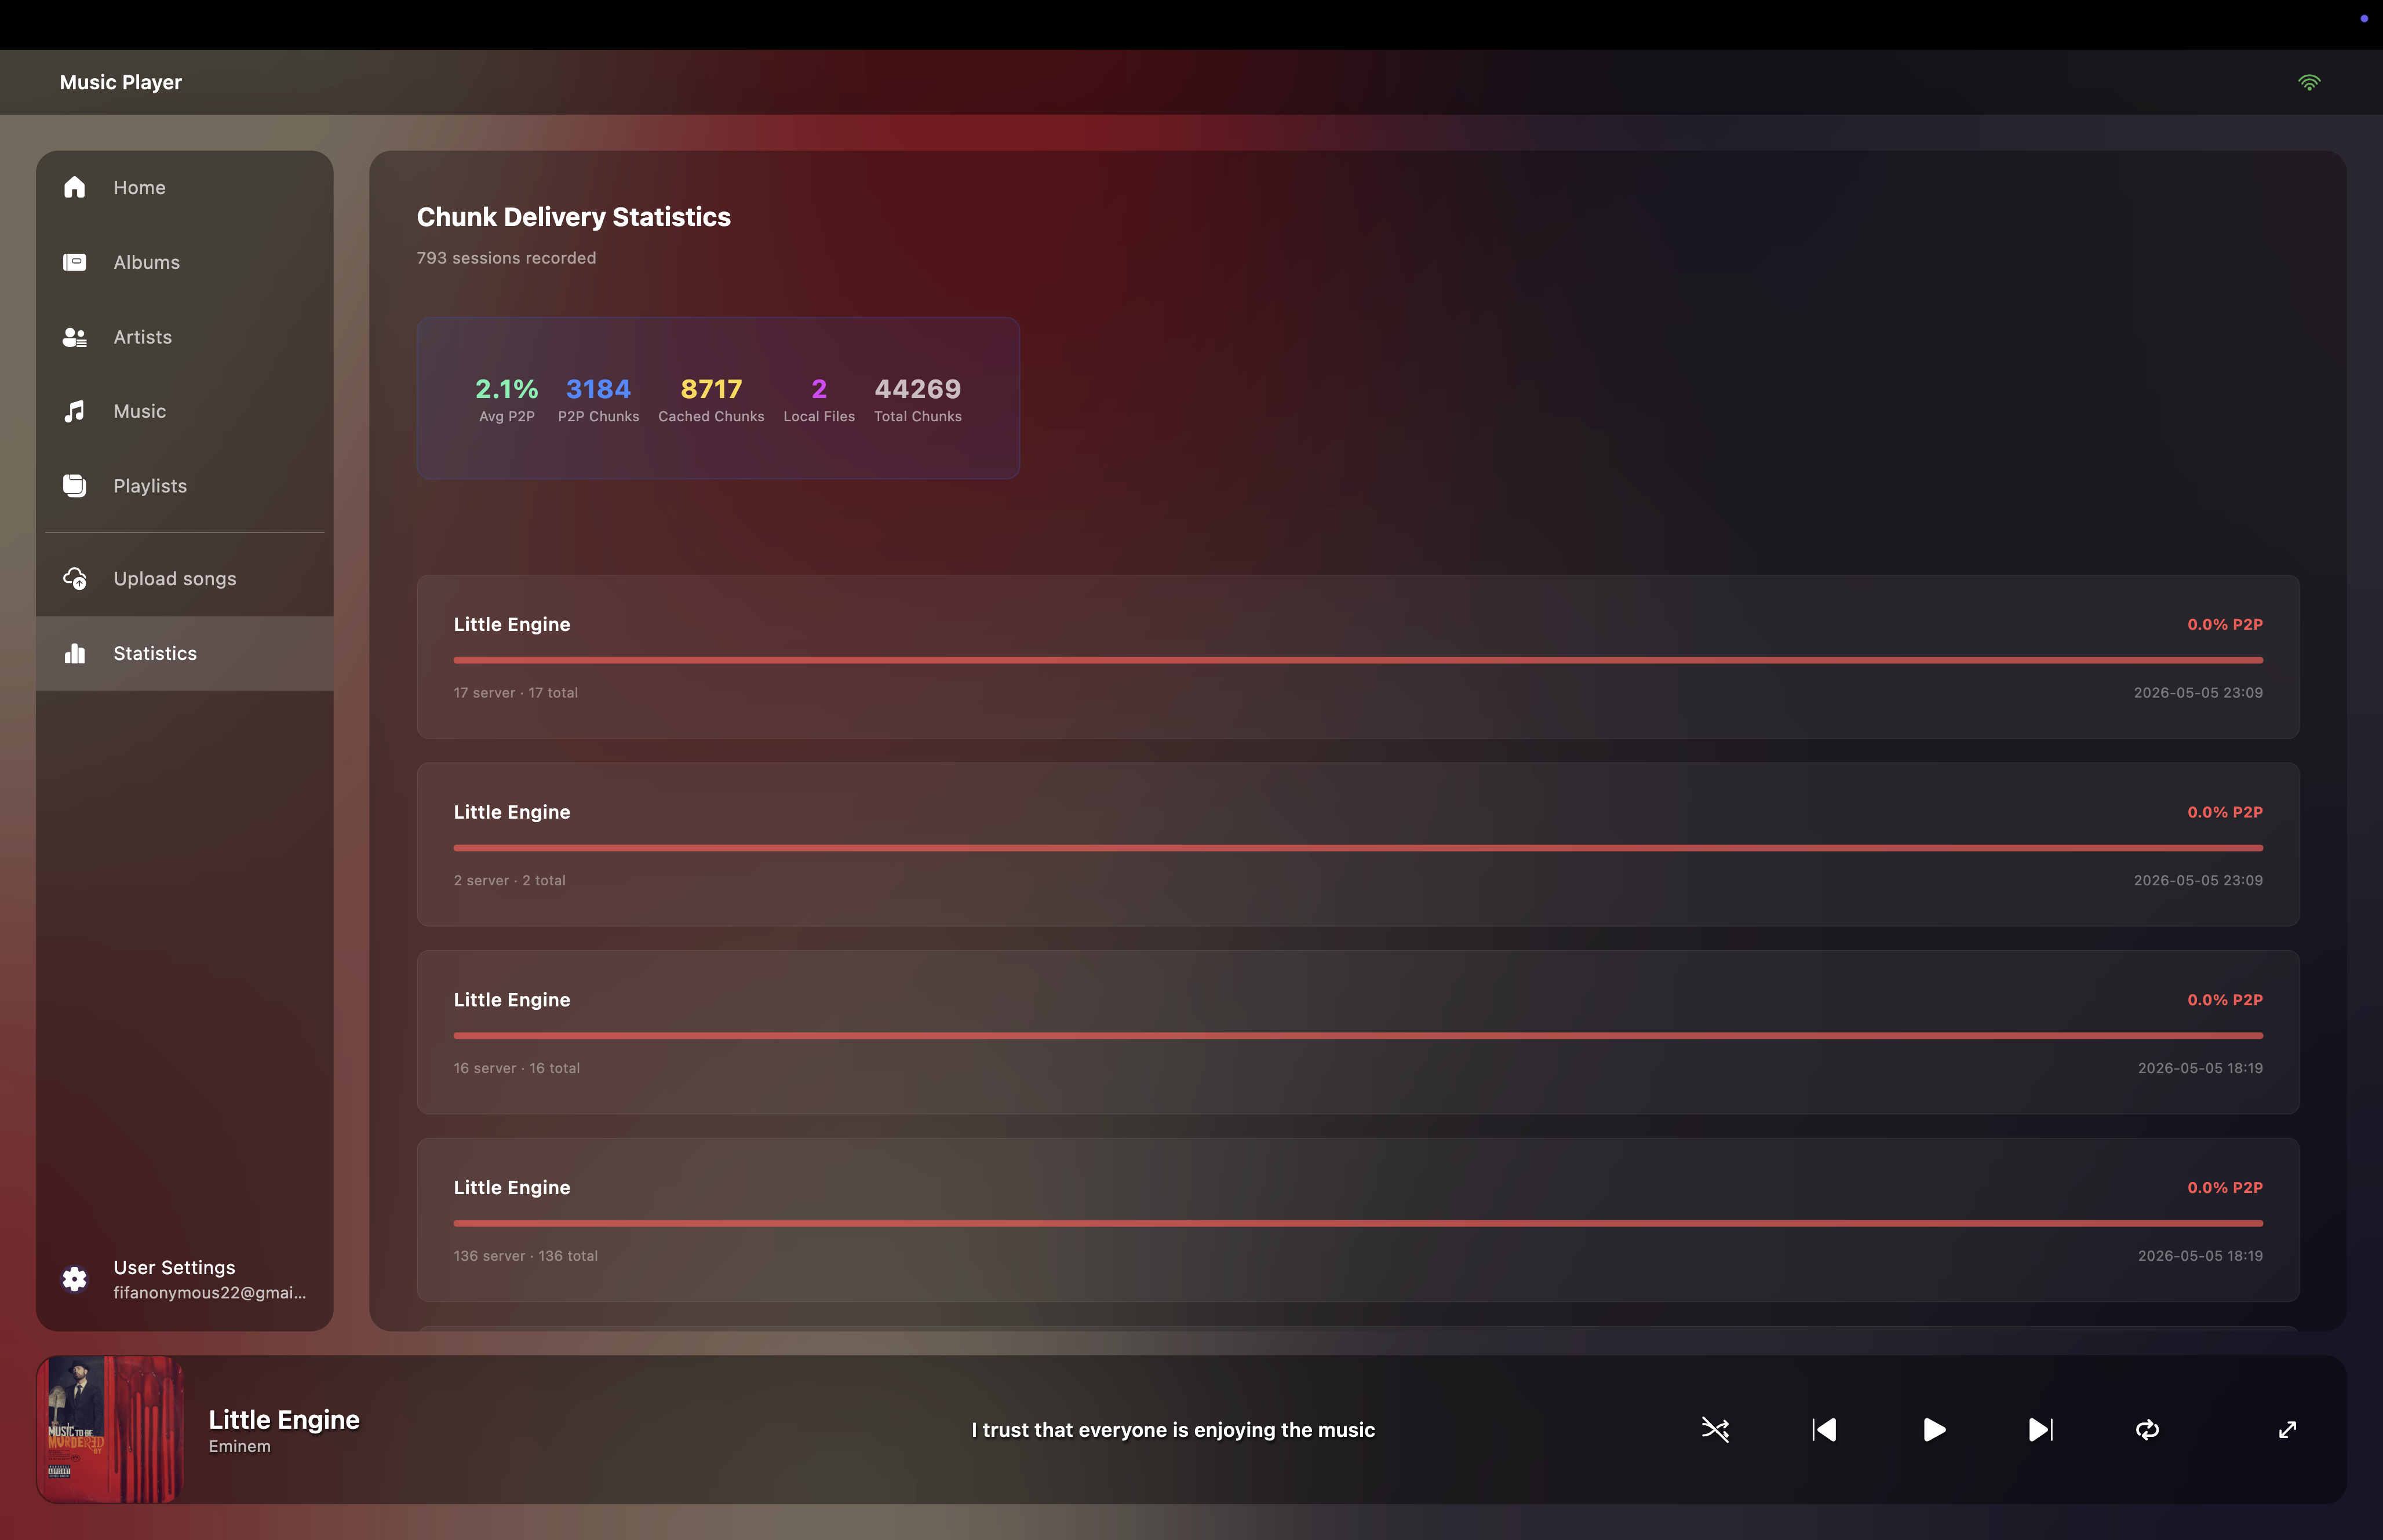
\includegraphics[width=\textwidth]{figures/screenshots/stats_screen.png}
\caption{Statistics screen with the aggregate card at the top and the per-session rows below.}
\label{fig:screen-stats}
\end{figure}


\section{Application Execution: Peer-Assisted Streaming}
\label{sec:exec-f1}

\indent \par This section walks through the main functionality of the application, the peer-assisted streaming, as a user would experience it from sign-in to verification. Each step below corresponds to one screenshot and to one observable effect on the system.

\subsection{Step 1: Reaching the Home Screen}
\label{subsec:exec-home}

\indent \par After the bootstrap completes (Sections \ref{sec:bootstrap}), the user lands on the home screen reproduced in Figure \ref{fig:exec-home}. At this point, the signaling WebSocket is already open, the access token has been refreshed, and the playback state has been pulled from \texttt{GET /playback}. The home rails are filled in from the recently played, recommended and rediscover endpoints, all of which read from the user library table.

\begin{figure}[htbp]
\centering
\includegraphics[width=\textwidth]{figures/screenshots/home_screen.png}
\caption{Home screen reached after the bootstrap completes, with the persistent player bar still showing the previously played song.}
\label{fig:exec-home}
\end{figure}

\subsection{Step 2: Selecting a Song}
\label{subsec:exec-select}

\indent \par From the drawer, the user opens the Music entry to reach the tracks view (Figure \ref{fig:exec-tracks}) and clicks on a song. The application calls \texttt{setQueueAndPlay} on the audio service, which builds the audio source and asks the chunk service for the manifest. On the first byte-range request, the service issues \texttt{GET /stream/\{fileHash\}/manifest} and, in parallel, \texttt{DISCOVER\_PEERS} over the signaling socket.

\begin{figure}[htbp]
\centering
\includegraphics[width=\textwidth]{figures/screenshots/tracks_screen.png}
\caption{Tracks view from which the user picks the song to play.}
\label{fig:exec-tracks}
\end{figure}

\subsection{Step 3: Playback Active}
\label{subsec:exec-playing}

\indent \par Tapping on the player bar expands it to the now playing screen, shown in Figure \ref{fig:exec-now-playing}. The first chunks (the 5\% prefix from equation \eqref{eq:prefix-impl}) are served by the origin server while the WebRTC handshake completes in the background. Once the data channel with the peer is open, the chunks above the prefix threshold are pulled directly from the peer; any peer timeout falls back transparently to the server, with the buffer absorbing the latency. The user sees only the smoothly advancing progress bar.

\begin{figure}[htbp]
\centering
\includegraphics[width=\textwidth]{figures/screenshots/expanded_music_player_widget.png}
\caption{Now playing screen during peer-assisted playback. The cover art, the lyrics, the queue and the progress bar are visible.}
\label{fig:exec-now-playing}
\end{figure}

\subsection{Step 4: Verifying Delivery on the Statistics Screen}
\label{subsec:exec-stats}

\indent \par When the song ends, or every 15 seconds during playback, the chunk service posts the cumulative counters to \texttt{POST /statistics}. To verify the result, the user opens the Statistics entry in the drawer, which produces the screen shown in Figure \ref{fig:exec-stats}. The aggregate card shows that, across all 793 sessions recorded so far, the application served on average 2.1\% of the bytes through peers, with the rest coming from the local cache (the dominant source in this single-user development setup) and from the origin server. The per-session list below the card breaks down each play and shows when peers were involved.

\begin{figure}[htbp]
\centering
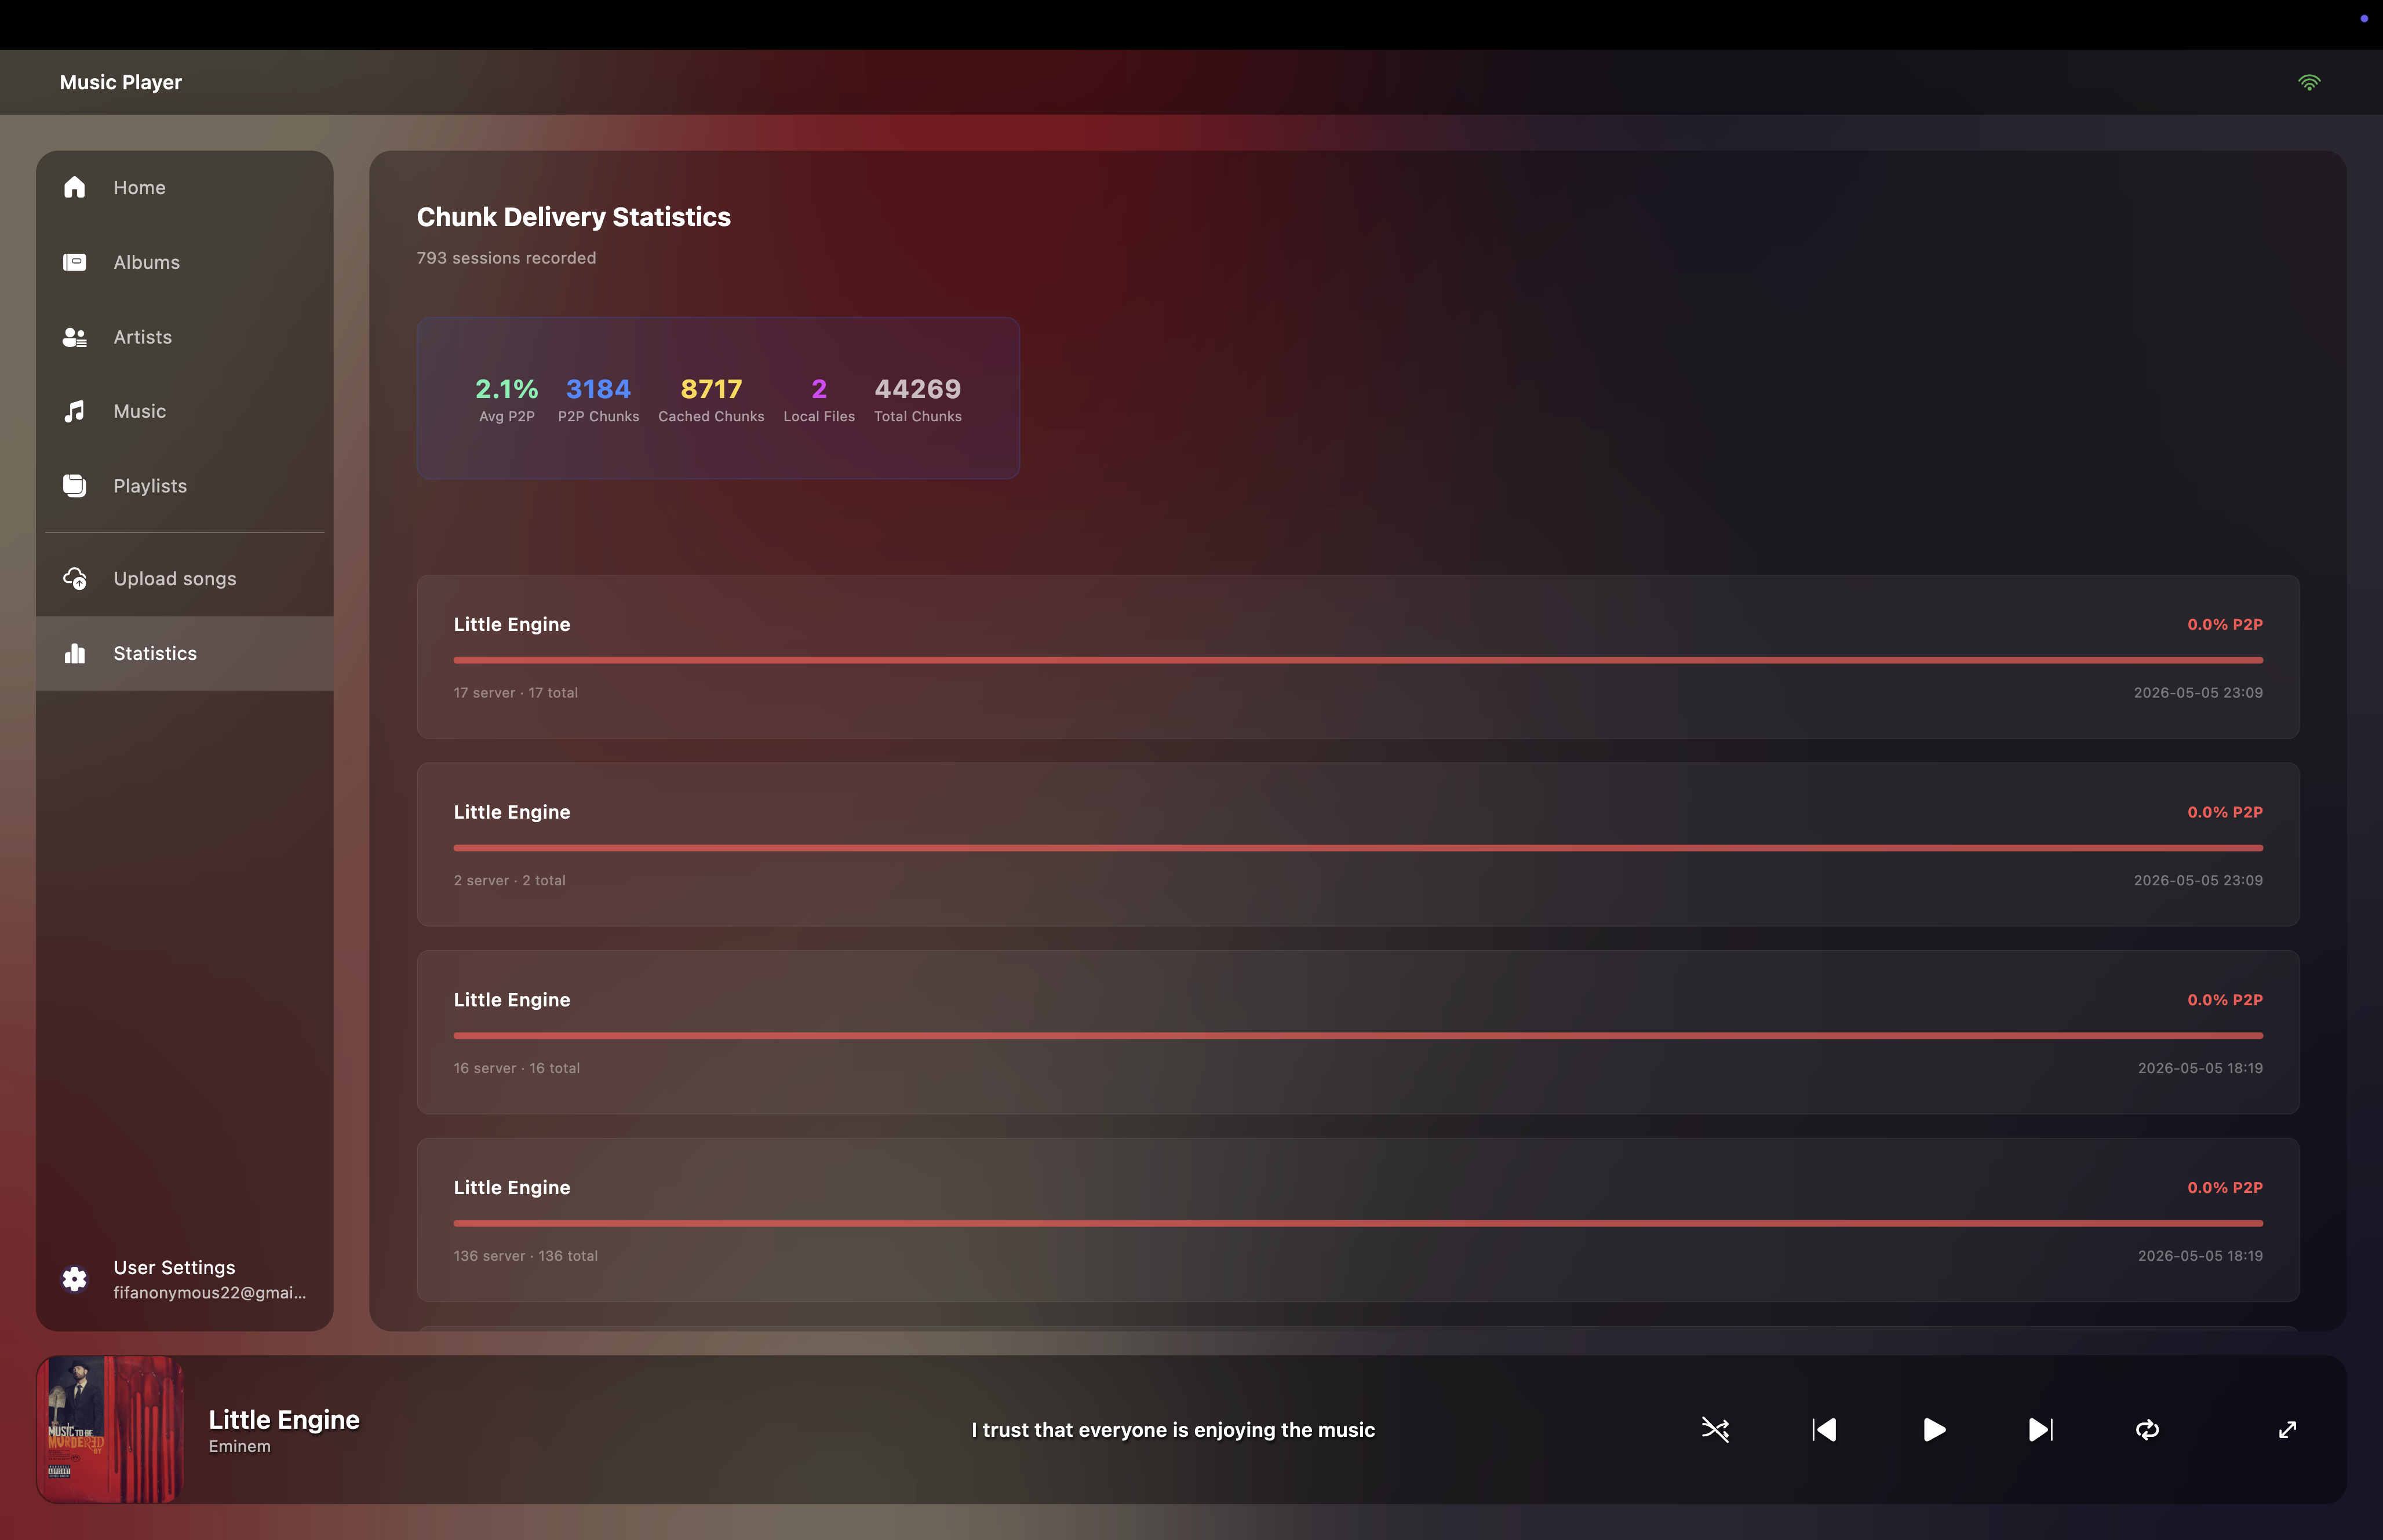
\includegraphics[width=\textwidth]{figures/screenshots/stats_screen.png}
\caption{Statistics screen after a streaming session, showing the aggregate offload card and the per-session breakdown.}
\label{fig:exec-stats}
\end{figure}

\par The relatively low average P2P share in Figure \ref{fig:exec-stats} is expected for this measurement setup, where most playback was performed by a single client with a warm local cache and no concurrent listener was available. Under more realistic deployment conditions, with several listeners playing the same song at the same time, the model in Chapter \ref{chap:ch2} predicts a much higher share, approaching the theoretical maximum.


\section{Mini User Manual}
\label{sec:user-manual}

\indent \par This section consolidates the steps above into a short reference. The numbers in parentheses point to the screenshots in Section \ref{sec:exec-f1}.

\begin{enumerate}
  \item Open the application and sign in with your email. The detailed authentication flow is described in Section \ref{subsec:auth}; once it completes, the home screen becomes visible (Figure \ref{fig:exec-home}).
  \item From the navigation drawer on the left, open the Music entry to reach the tracks view (Figure \ref{fig:exec-tracks}). You can also browse the catalogue through the Albums, Artists or Playlists entries.
  \item Click on a song. Playback starts almost immediately because the very first chunks are served by the origin server while the peer connections are still being negotiated. If other listeners are connected and have parts of the same song cached, the rest of the chunks are pulled directly from them; otherwise, the server keeps serving the song.
  \item Tap on the player bar at the bottom of the screen to open the now playing view (Figure \ref{fig:exec-now-playing}). From here you can pause, resume, skip, seek, toggle shuffle and repeat, and like the song.
  \item To upload your own songs, open the Upload songs entry in the drawer (Figures \ref{fig:screen-upload-empty} and \ref{fig:screen-upload-song}), pick the files from disk, and press Upload. The application will only transfer the chunks that the server does not already have.
  \item To control how much data the application uses for peer uploads, open the User Settings entry in the drawer (Figure \ref{fig:screen-settings}) and adjust the Peer Network dropdown together with the WiFi and Cellular data limits.
  \item To verify how much of your listening was served by peers versus by the server, open the Statistics entry in the drawer (Figure \ref{fig:exec-stats}). The aggregate card on top sums up every session, and the rows below it break each one down individually.
\end{enumerate}

\chapter{Conclusions and Future Work}
\label{chap:ch5}

\tolerance=9999
\emergencystretch=3em

\indent \par This thesis began with an awkward observation: on a cloud-hosted streaming service the bytes of a song are paid for twice, and the second payment, the egress out of the data center, grows with the number of people listening rather than with the revenue they bring. The more a track is loved, the more it costs to serve. Sitting unused inside that problem was a delivery network made of the listeners themselves, since anyone who has just heard a piece of a song holds a copy that the next listener is about to need. The question the rest of the thesis set out to answer was whether that latent network could be put to work without the listener ever noticing, which meant satisfying three constraints at once: playback had to start instantly, the same code had to run in a browser and on a phone, and a piece of audio handed over by an untrusted peer had to be exactly as safe as one fetched from the server.

\par On the evidence gathered in Chapter \ref{chap:ch4}, the answer is yes, with the caveats that a prototype always carries. The chapters between the question and this one built the argument, the system and the measurement in turn, and they line up against the three constraints and the cost goal as follows.

\indent \par The cost goal was the reason for the whole exercise, and it is the one the measurements speak to most directly. Chapter \ref{chap:ch2} derived an offload ceiling of $\rho = 1 - P/S$ and argued that a peer-assisted swarm moves the origin away from serving $O(N)$ complete streams of the same song. Chapter \ref{chap:ch4} measured a warm two-to-five-client swarm serving 88.4\% of its bytes from peers and only 11.6\% from the origin, and, once a signaling concurrency defect was found and fixed, that server share stayed flat as the swarm grew from one listener to five. A flat share is the concrete form of the claim in this prototype: the origin's involvement in any one listener's stream does not grow with the size of the audience. The figure lands in the same regime as the 8.8\% that Kreitz and Niemel\"a measured for Spotify's production system \cite{spotify_p2p}, which is the closest external point of reference that exists, and the gap between the two is accounted for by the cold cache of the prototype rather than by any difference in the mechanism.

\par The instant-playback constraint was met by the prefix. A dynamic prefix of about 5\% of each song, served from the origin, hides the WebRTC connection setup, which the measurements put at a median of 243 milliseconds, comfortably inside the eleven seconds of audio that the prefix buys. Click-to-sound therefore stays at the level of an ordinary server stream even though the bulk of the song arrives over a peer connection that did not exist when the user pressed play. The cross-platform constraint was met by building the client once, in Flutter, and running it unchanged on Linux, macOS, Windows, Android, iOS and, through a Service Worker, the web browser. The integrity constraint was met by content-addressing every 64 KiB chunk with its SHA-256 hash, so that a chunk is verified identically whether it came from a peer or the origin, and a failed verification simply falls back to the server. That fallback, rather than a TURN relay, is also what the system uses when a direct peer connection cannot be established, which keeps the cost-saving property of the peer model intact: a relayed byte would be billed exactly like a server byte.

\par It is worth being equally clear about what was not shown. The measurements were taken on a single machine over the loopback interface, with one synthetic track and listeners that always started cold, so the offload and the setup latency are best-case figures and the absolute savings are too small to quote in money. The cache share that dominates a mature deployment was zero by construction. The evaluation is therefore a demonstration that the mechanism behaves as the model predicts under controlled conditions, not a measurement of a production service. What it does establish, and what the introduction asked for, is that the latent delivery network can be put to work, that the origin can be reduced from serving the whole song to serving a small bootstrap and fallback role, and that the price of doing so, paid in a small server prefix and a few hundred milliseconds of background connection setup, need not be visible to the listener at all.

\indent \par The most valuable next step is also the most obvious one: repeat the evaluation outside the laboratory. Running the swarm across several machines on a real wide-area network, with non-trivial round-trip times and genuine NAT traversal, and over a realistic catalogue of varied music rather than a single tone, would turn the share-based results of Chapter \ref{chap:ch4} into a saving that can be quoted in currency and would expose the system to the cross-platform connection failures that the loopback interface never provokes. Warm-cache and larger-swarm runs belong in the same effort, since the cache share that this thesis measured as zero is precisely the contribution that grows to dominate a mature peer-assisted service \cite{spotify_p2p}, and the flash-crowd behaviour at large $N$, which the signaling fix addressed only at the small scale tested here, still needs to be characterised.

\par A second strand concerns resilience and reach. The cross-platform connectivity limitation of Section \ref{sec:limitations}, where browsers hide their local addresses behind mDNS hostnames that native peers cannot always resolve, is the clearest barrier to mixed browser-and-mobile swarms offloading as well as desktop pairs, and is worth attacking directly. The signaling WebSocket should reconnect on its own with a backoff loop rather than waiting for the next user action, so that a device is never silently absent from the swarm. On mobile, where seeding spends battery and metered data, the simple network-mode and monthly-cap controls implemented here could grow into a policy informed by charging state and connection type, and possibly into an incentive scheme, building on the prior characterisations of mobile peer-assisted streaming and of device-to-device communication \cite{spotify_mobile_p2p,d2d_survey}.

\par A third strand is about turning design arguments into further measurements and about the product itself. The prefix size and the peer timeouts were chosen on the strength of the cost model and fixed in code. Making them dynamic or exposing them as parameters would let the trade-offs that Chapter \ref{chap:ch2} reasoned about be swept and measured rather than argued. Beyond performance, a peer learns something about what its neighbours are listening to when it serves them chunks, so a privacy-preserving request scheme is a natural and important extension, and a relay tier could be offered, as a deliberate paid option rather than a default, to the small fraction of users for whom direct connectivity never succeeds \cite{relays_turn}.

\par A fourth, more ambitious strand is interoperability with other music streaming services and local media players. In the current prototype, cached audio is stored as separate verified chunks rather than as a normal playable audio file, so a song reconstructed from the cache cannot be opened directly by another application. Future work could explore a reconstruction layer that joins the cached chunks back into a conventional media file when enough of them are available, while still preserving the chunked layout needed for peer delivery. This would make the same stored data useful both inside MP33r and outside it, but it would have to be designed carefully so that file reconstruction, local media scanning and direct-file playback do not slow down the streaming path.

\par None of these changes the shape of the result. They widen the conditions under which it has been shown to hold. The core finding stands: the listeners of a song are, collectively, most of the infrastructure needed to deliver it, and a system can draw on that infrastructure while keeping playback instant, the catalogue safe and the code single-sourced across platforms. The opening worry was that the more a song is loved, the more it costs to serve. The system built here turns the same fact into an asset, because the more a song is loved, the more listeners there are holding a copy of it and the more hands are there to pass it along.


%\addcontentsline{toc}{chapter}{Concluzii}
%\addcontentsline{toc}{chapter}{Conclusions}

\bibliography{references}

\end{document}
